\chapter{NOvA Test Beam detector calibration}\label{sec:TBCalibrationSection}

In this chapter I describe the details of the Test Beam detector calibration as it was finalized in June 2023. This version includes a new purpose-made data-based simulation of cosmic muons as described in Chapter~\ref{sec:DataBasedSimulation} and all the measured Test Beam data, with the exception of the period 1 data.

The data calibration samples for Test Beam were created using the same procedures as the \gls{ND} and \gls{FD} calibration samples, described in Sec.~\ref{sec:NOvACalibration}. However, there are two cuts from the event election, that were not included for Test Beam during the processing of the data samples. This can be seen on Tab.~\ref{tab:DataBasedSimEventSelection}, where the two bottom rows show the two excluded cuts. One cut contains the vertex close to the edge of the detector ensuring we only use cosmic events, the other contains the end of track close to the edge, ensuring we only use through-going muons for the relative calibration. Given that we remove beam events and that all the other cuts are designed to select cosmic events, the first cut has only a negligible effect on the final selection. Additionally, the stopping muons only make up a small fraction of the total cosmic muon events, rendering the second cut also negligible.

This section is organized as follows. I first describe the Test Beam versions of the fibre brightness map in Sec.~\ref{sec:FibreBrightnessTB} and the threshold and shielding correction in Sec.~\ref{sec:TBThresholdCorrection}, as they were introduced in Sec.~\ref{sec:NOvACalibration}. I then go over the simulation sample and the three data samples (for periods 2, 3, and 4) in Sec.~\ref{sec:SimulationResults}-\ref{sec:TBPeriod4}, showing distributions of hits selected for calibration and of the uncorrected energy deposition before calibration. I discuss considerations going into calibration, including splitting the individual periods into smaller samples, or describing issues that could affect the calibration results.  Afterwards, I am showing a selection of attenuation fit results for each sample together with an overview of the relative calibration effects. Lastly, I discuss the absolute calibration results in Sec.~\ref{sec:TBAbsoluteCalib} for all the samples combined, as well as the validation and conclusion of the Test Beam calibration in Sec.~\ref{sec:TBCalibValidation} and \ref{sec:TBCalibSummary} respectively.

%Temperature study (small overview - probably not needed at all, depends if Randeeth want to add his work to this technote)

%From Teresa's thesis
%Along with setting the energy scale of the detector, we need to calibrate the timing of the readout system for the detector. The Data Concentrator Modules (DCMs) responsible for collating the data from multiple FEBs get their timing information via a daisy chain originating at the detector TDU. Each DCM in the chain has a timing offset relative to the DCM before it, with the last DCM having the earliest ti. Following the procedure described in [66], I used timing information from hits on cosmic ray muon tracks that pass through multiple DCMs to determine the relative offsets between DCMs, shown in Figure 3.20.

%From Teresa's thesis:
%"For Test Beam, we have three beam-based triggers, one pulsed trigger, and two data-driven triggers. The data-driven triggers are both activity-based triggers. The first is intended to record cosmic ray induced events for use in calibrating the detector.

\section{Fibre brightness}\label{sec:FibreBrightnessTB}

To divide the Test Beam detector into \gls{FB} bins we use the attenuation fit results for Test Beam period 4 data (described in Sec.~\ref{sec:TBPeriod4}), as that is the best detector conditions data we have. Since we need the \gls{FB} map in order to run the attenuation fits and we need the attenuation fit results to create the \gls{FB} map, we proceeded iteratively. We first run the attenuation fit with an older version of the \gls{FB} map and use the results to create a new \gls{FB} map, discussed here, which is then used in a new attenuation fit.

We are only using the attenuation fit results in the centre of each cell to create the \gls{FB} map, therefore, we decided to allow some cells that failed the calibration condition ($\chi^2>0.2$), to be still used for the creation of the \gls{FB} map. Otherwise, all the officially uncalibrated cells are assigned an average response across the entire detector, resulting in a loss of information on their relative brightness. As can be seen in Fig.~\ref{fig:FiberBrightnessExamples}, some attenuation fits have $\chi^2>0.2$, even though they correctly represent the energy deposition in the centre of that cell. By carefully investigating all the uncalibrated Test Beam cells (doable for Test Beam, due to its small number of cells), we concluded that all the cells with $\chi^2<0.7$ can be used to create the \gls{FB} map, since the response in their centre is described reasonably well by their attenuation fits. We use this loosened calibration condition only to create the \gls{FB} map and we keep the original condition for the actual calibration results.

%Describe and show plots that since we are only using the fitted response at cell centre we can allow fits with $\chi^2>0.2$. Show examples of responses with chisq larger than that and say what is the final chisq chosen. No need to show the final distribution of the fb bins here as they were technically shown in the general calibration description. But might refer back to it...

\begin{figure}[h]
\centering
\begin{subfigure}[b]{0.495\textwidth}
\centering
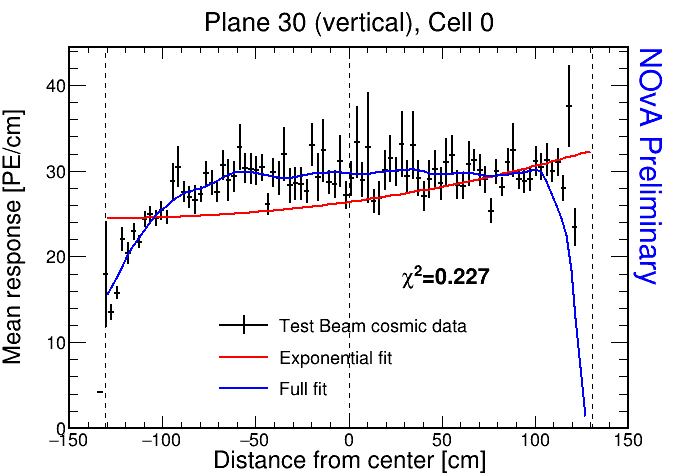
\includegraphics[width=\textwidth]{Plots/TBCalibration/ExampleForBrightFile_fb0_030_000.png}
\end{subfigure}
%\hfill
\begin{subfigure}[b]{0.495\textwidth}
\centering
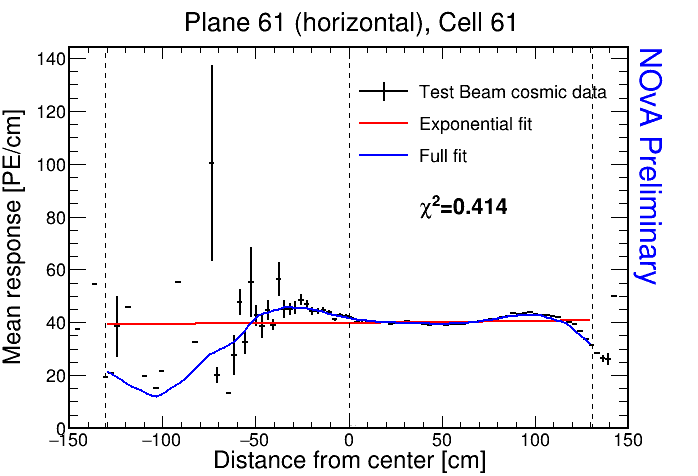
\includegraphics[width=\textwidth]{Plots/TBCalibration/ExampleForBrightFile_fb5_061_061.png}
\end{subfigure}
\caption[Example of failed attenuation fits used for the Test Beam fibre brightness file]{Examples of attenuation fits for two cells that fail the calibration condition, but the fit (blue line) still correctly represents the energy deposition in the centre of that cell (dashed vertical line in the middle). The total $\chi^2$ between the data (black) and the attenuation fit for both plots are included.}
\label{fig:FiberBrightnessExamples}
\end{figure}

The final distribution of relative \gls{FB} values that are used to populate the \gls{FB} bins for the Test Beam detector is shown in Fig.~\ref{fig:TBFiberBrightnessMap}. The resulting map of \gls{FB} bins and their corresponding relative brightnesses was shown in the previous chapter in Fig.~\ref{fig:NOvAFiberBrightness}.

\begin{figure}[hbtp]
\centering
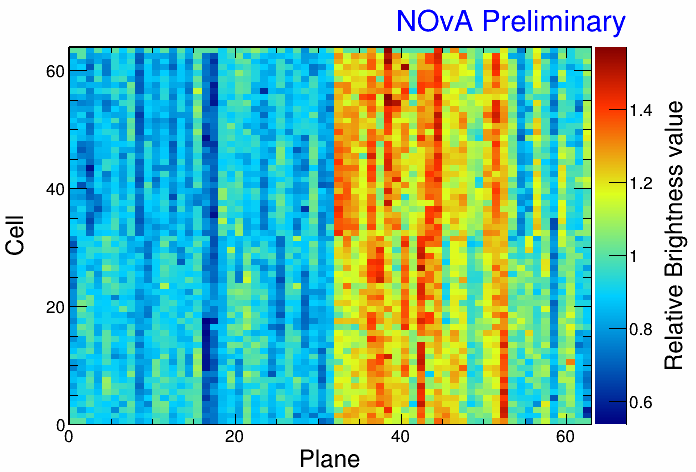
\includegraphics[width=.8\textwidth]{Plots/TBCalibration/TBFiberBrightnessMap.png}
\caption[Fibre Brightness map for the Test Beam detector]{\acrshort{FB} map representing relative differences in energy response due to different brightnesses of the fibres, scintillators, or readout. Create from the attenuation fit results of the \acrshort{NOvA} Test Beam detector with a shifted calibration condition from $\chi^2<0.2\rightarrow 0.7$ to enable using the attenuation fits that are officially uncalibrated, but correctly represent energy deposition in cell centre. Otherwise, all the uncalibrated cells get assigned a mean detector response, represented by number 1 on this map.}
\label{fig:TBFiberBrightnessMap}
\end{figure}

\section{Threshold and shielding corrections}\label{sec:TBThresholdCorrection}
%Describe in generall what is TS correction for
The threshold and shielding correction is intended to mitigate biases arising from differences between cosmic events used for calibration and beam events. It is only used prior to the attenuation fits and is omitted when applying the results of the relative calibration, whether during the absolute calibration or for beam events. Additionally, it is derived exclusively from simulation.

%TS correction dependence on w
We created a new threshold and shielding correction for the Test Beam detector using the new simulation described in Sec.~\ref{sec:DataBasedSimulation}. The correction is calculated for both views, across 12 \gls{FB} bins, 64 cells, and 100 $w$ bins, where $w\in\left(\unit[-130]{cm},\unit[130]{cm}\right)$. Two examples of the correction as a function of $w$ are shown in Fig.~\ref{fig:TBThresholdCorrectionExamples}, demonstrating an almost uniform behaviour along a cell. Relative variations of the correction in the X view range from $\unit[1-2]{\%}$,  primarily concentrated at the edges of the cell. In the Y view, the correction exhibits sub-$\unit[1]{\%}$ variations. These trends are consistent across all the \gls{FB} bins and views. Given that the threshold and shielding correction precedes relative calibration, the absolute value of the correction is irrelevant and only the relative variations along $w$ and between cells matter.
 
\begin{figure}[!hbtp]
\centering
\begin{subfigure}[t]{\textwidth}
\centering
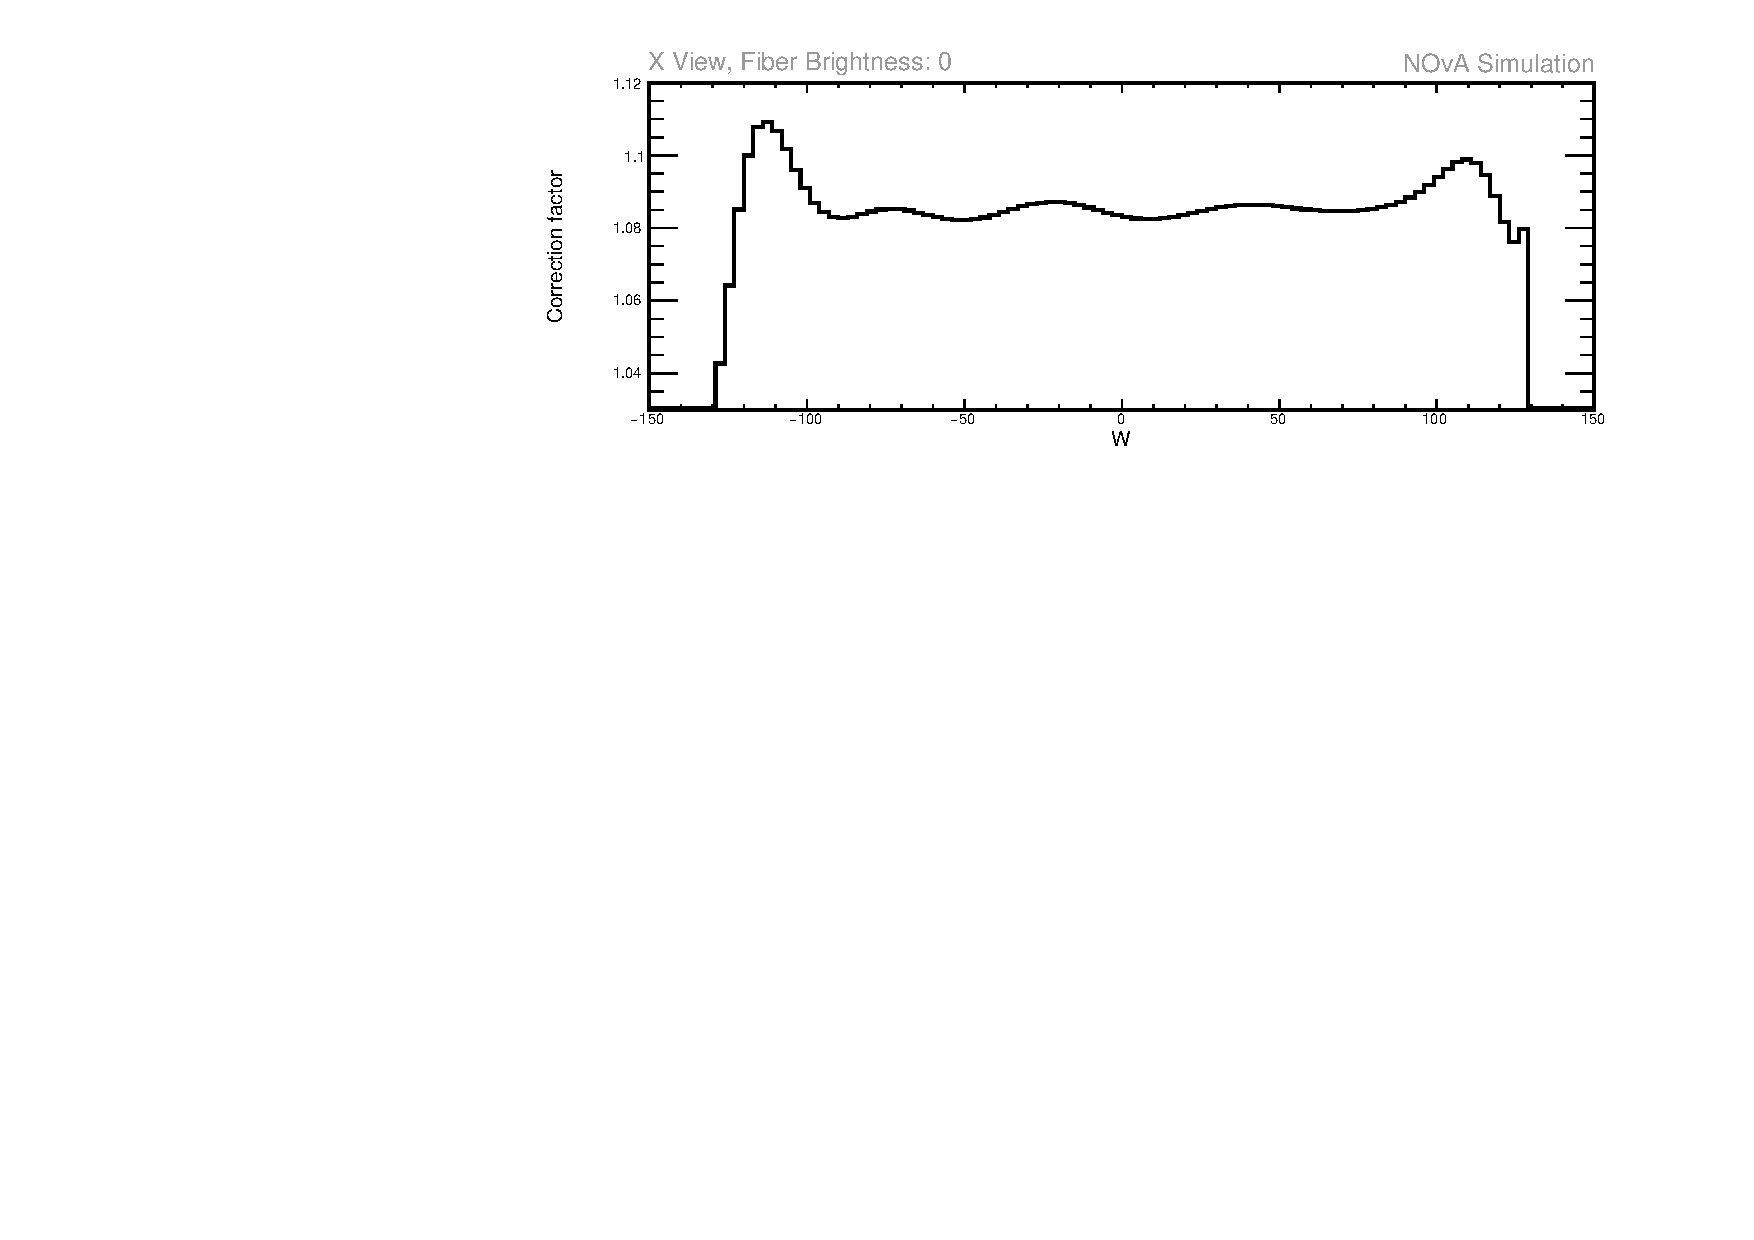
\includegraphics[width=\textwidth]{Plots/TBCalibration/ThresholdCorrectionExample_axview_fb0_P4DataBasedSim.pdf}
\end{subfigure}
\begin{subfigure}[b]{\textwidth}
\centering
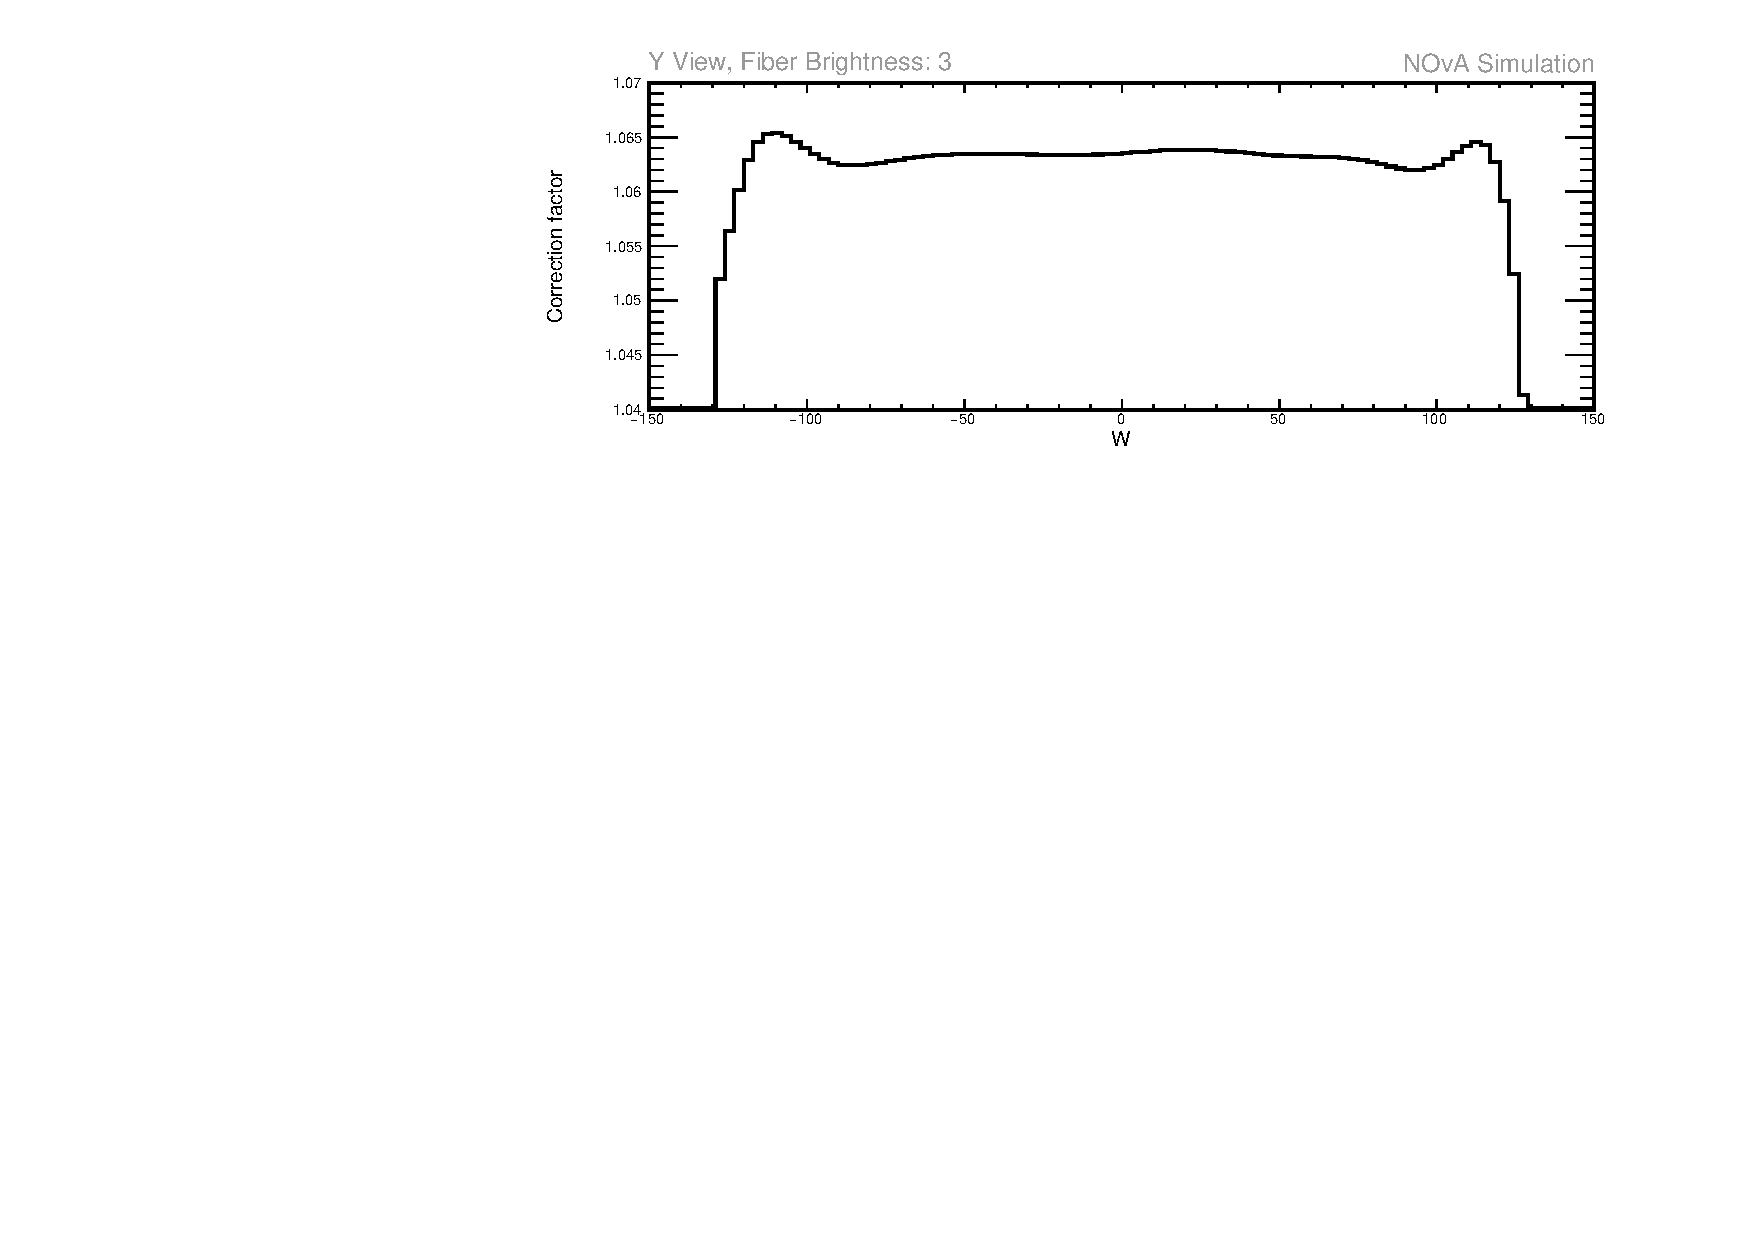
\includegraphics[width=\textwidth]{Plots/TBCalibration/ThresholdCorrectionExample_ayview_fb3_P4DataBasedSim.pdf}
\end{subfigure}
\caption[Example threshold and shielding correction for Test Beam detector]{Examples of threshold and shielding corrections as a function of the position within a cell in X view (top) and Y view (bottom) for the Test Beam detector.}
\label{fig:TBThresholdCorrectionExamples}
\end{figure}

%Where do the variations come from?
This uniformity of the distributions is expected, considering the relatively small size of the Test Beam detector compared to the \gls{FD}, which prompted the investigation into threshold and shielding effects. The Test Beam detector's cell length of $\unit[2.6]{m}$ has only a negligible impact on the threshold saturation or on the energy distribution of cosmic muons, resulting in  the uniformity of the threshold and shielding correction for Test Beam detector. The larger correction at cell edges is likely caused by lower event counts in those areas. However, since this relative sparsity of events also influences relative calibration due to large variation in the energy response, the relatively larger threshold and shielding correction at cell edges is not detrimental.

%Dependence of the TS correction on plane and cell
The distribution of the threshold and shielding correction across Test Beam detector's cells and planes, shown in the top of Fig.~\ref{fig:TBThresholdCorrectionMap}, demonstrates, that while the correction is expected to be generally uniform across the detector, there are notable variations between cells and planes forming a discernible pattern. These variations and their shape primarily stem from the threshold component of the correction, shown in the bottom of Fig.~\ref{fig:TBThresholdCorrectionMap}.

\begin{figure}[!hbtp]
\centering
\begin{subfigure}[t]{\textwidth}
\centering
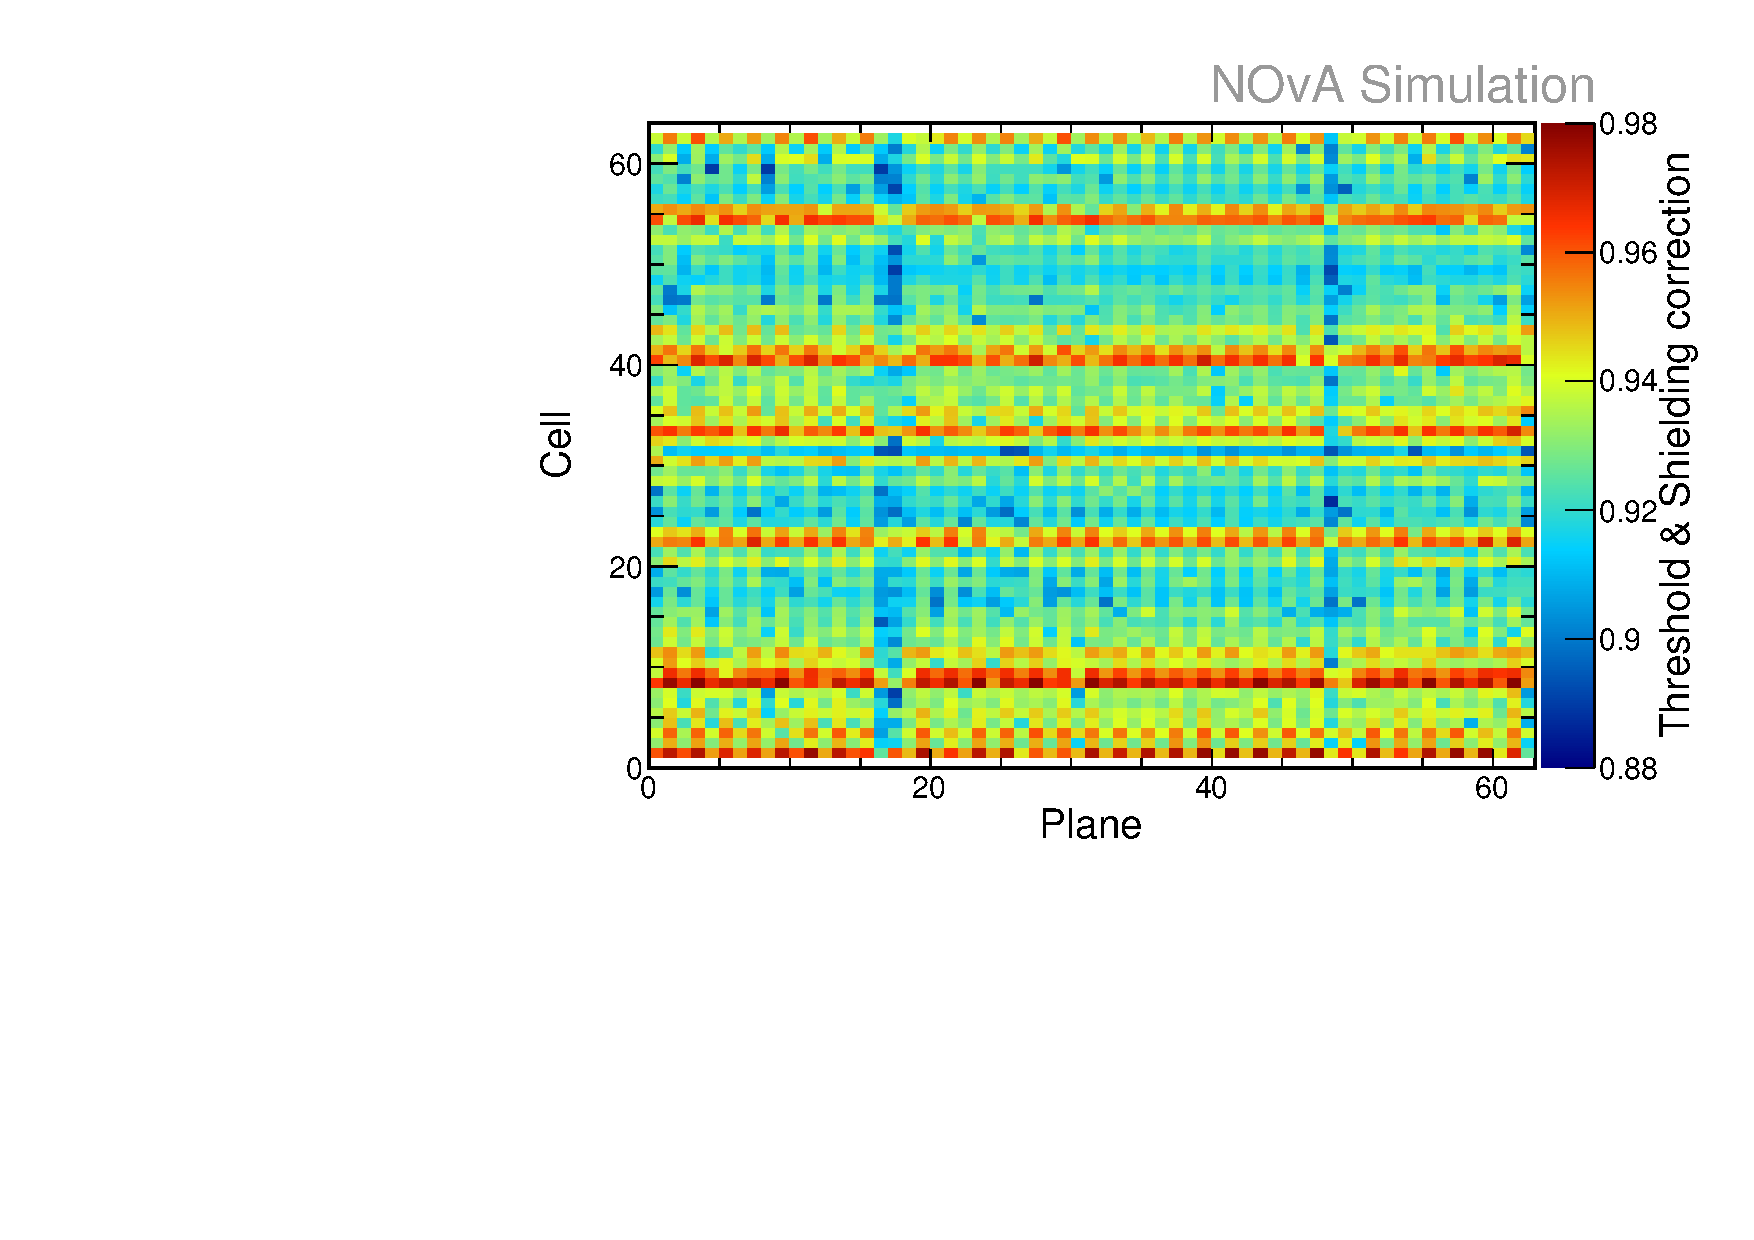
\includegraphics[width=.8\textwidth]{Plots/TBCalibration/ThresholdCorrectionMap_P4DataBasedSim.pdf}
\end{subfigure}
\begin{subfigure}[b]{\textwidth}
\centering
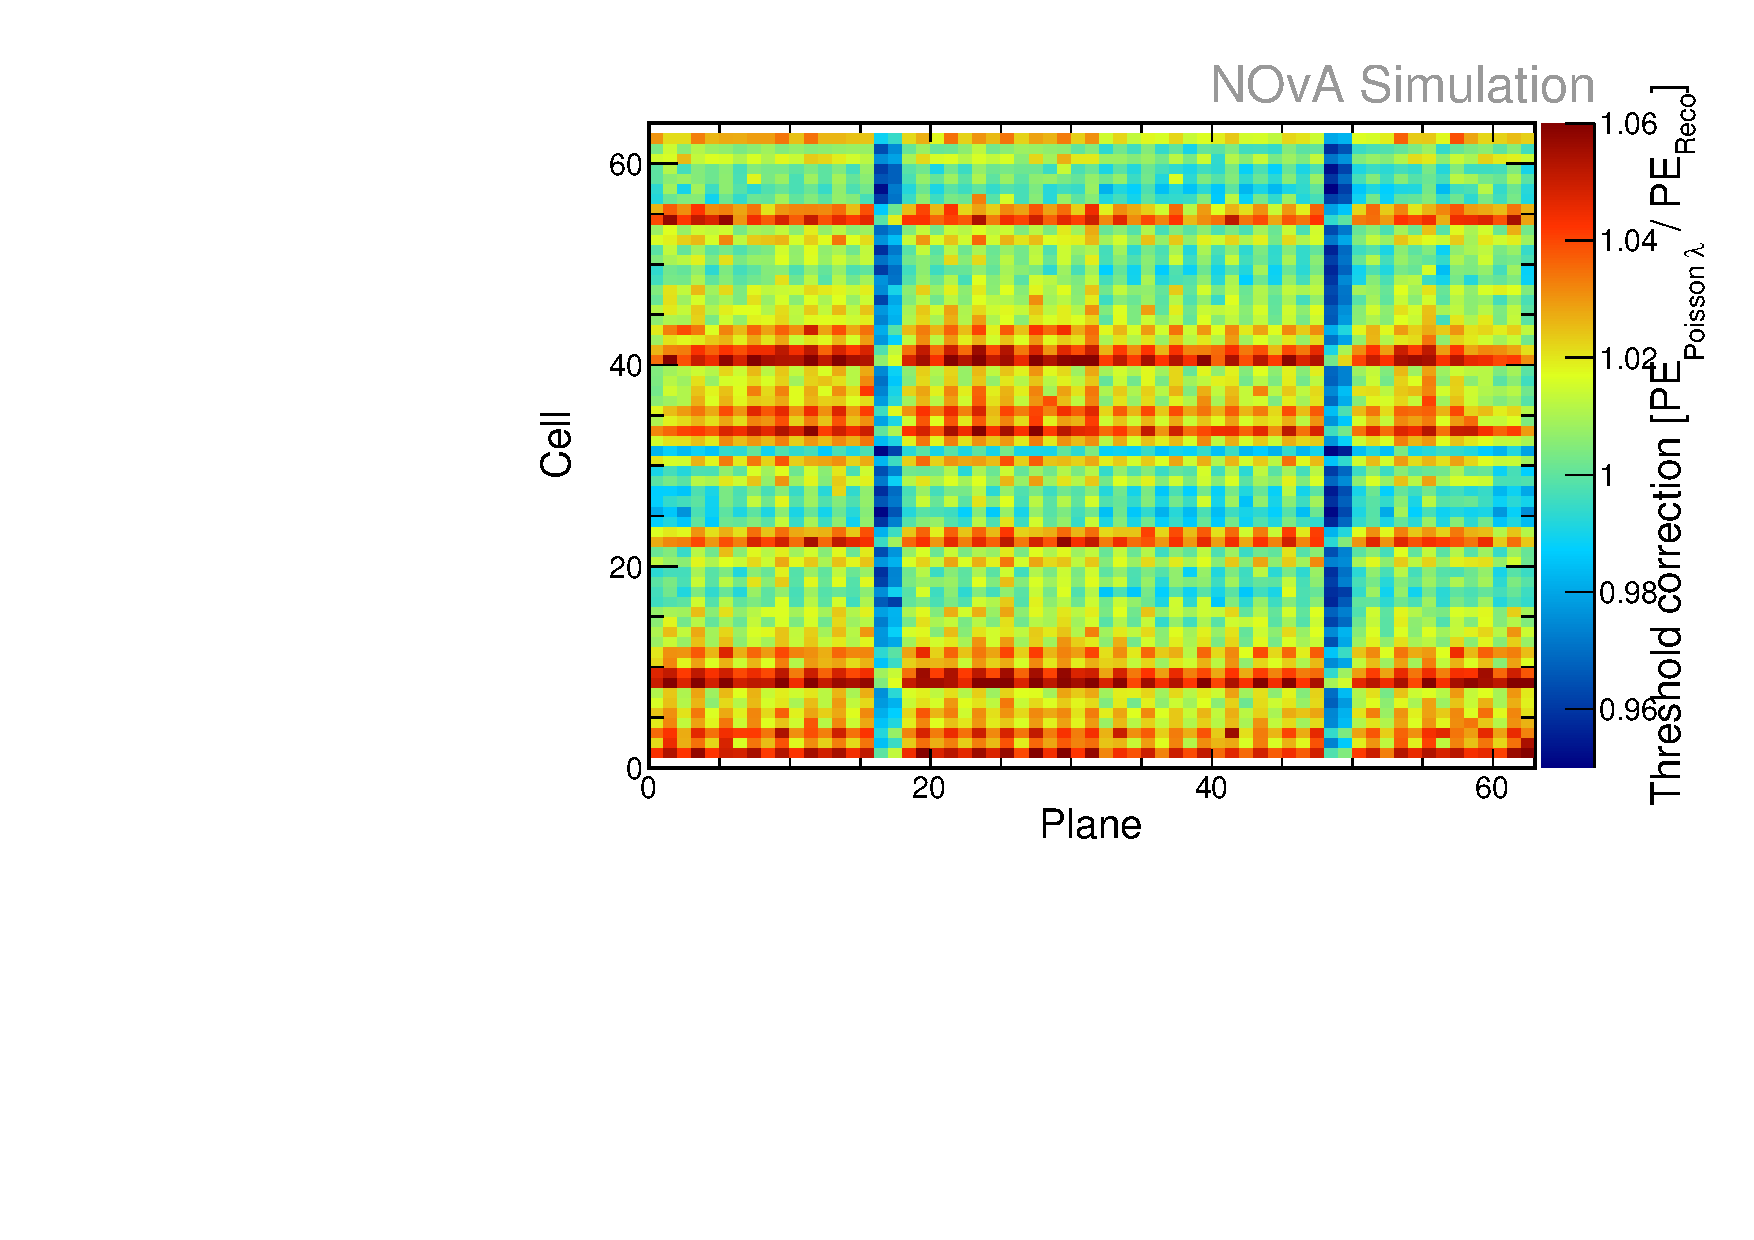
\includegraphics[width=.8\textwidth]{Plots/TBCalibration/ThresholdOnlyCorrectionMap_P4DataBasedSim.pdf}
\end{subfigure}
\caption[Map of the threshold and shielding correction across the Test Beam detector]{Map of the threshold and shielding correction (top) and only of the threshold part of the correction (bottom) as a function of the Test Beam detector's cell and plane number. Each bin shows the mean correction for all the simulated events in that cell.}
\label{fig:TBThresholdCorrectionMap}
\end{figure}

%What is the threshold correction
The threshold part of the correction can be expressed as
\begin{equation}
\textsf{Threshold correction}=\frac{\gls{PE}_{\mathrm{Poisson}\lambda}}{\gls{PE}_{\mathrm{Reco}}},
\end{equation}
where $\gls{PE}_{\mathrm{Poisson}\lambda}$ represents the mean of the Poisson distribution of the true deposited energy (in terms of $\gls{PE}_{\mathrm{True}}$), and $\gls{PE}_{\mathrm{Reco}}$ is the reconstructed number of \gls{PE} from simulation. Both $\gls{PE}_{\mathrm{Poisson}\lambda}$ and $\gls{PE}_{\mathrm{True}}$ are direct outputs of the light model simulation, as detailed in Sec.~\ref{sec:NOvASimulation}. After the light model simulation, $\gls{PE}_{\mathrm{True}}$ is passed through the readout simulation, which includes a \gls{PE}-to-\gls{ADC} function for calculating the peak \gls{ADC} value. This value is then converted into $\gls{PE}_{\mathrm{Reco}}$ using the \gls{ADC}-to-\gls{PE} scale described in Sec.~\ref{sec:NOvACalibration}. The observed shape in the threshold correction can thus be attributed to differences between $\gls{PE}_{\mathrm{True}}$ and $\gls{PE}_{\mathrm{Poisson}\lambda}$, as well as to various effects introduced by the readout simulation. However, the differences between $\gls{PE}_{\mathrm{True}}$ and $\gls{PE}_{\mathrm{Poisson}\lambda}$ are marginal (below $\unit[1]{\%}$) and contribute minimally to the threshold correction. Therefore, the predominant influence on the observed pattern comes from the effects introduced by the readout simulation.

%FEB versions
There are two prominent features in the threshold correction variations in Fig.~\ref{fig:TBThresholdCorrectionMap}. Firstly, the two blue vertical lines in planes 16-17 and 48-49. These planes are using the \gls{FEB} version 5.2, used in the \gls{ND}, instead of  the \gls{FEB} version 4.1, used in the \gls{FD} and in all the other Test Beam planes, as explained in Sec.~\ref{sec:TBExperiment}. Both the readout simulation and the \gls{ADC}-to-\gls{PE} scale do account for the expected disparity in the \gls{ADC}/\gls{PE} ratio between the two \gls{FEB} versions. However, it is expected that \gls{FEB}v5 would exhibit a lower response to the same energy compared to \gls{FEB}v4. Therefore, for the same $\gls{PE}_{\mathrm{Poisson}\lambda}$ values, the $\gls{PE}_{\mathrm{Reco}}$ for \gls{FEB}v5 should be smaller than that for \gls{FEB}v4. Consequently, the \gls{FEB}v5 planes should have a larger threshold correction compared to the \gls{FEB}v4. However, as was shown in Fig.~\ref{fig:TBThresholdCorrectionMap}, the observed correction is contrary to this expectation, suggesting a potential error in the readout simulation regarding the handling of different \gls{FEB} versions.

%APD relative gain map
The second notable feature in Fig.~\ref{fig:TBThresholdCorrectionMap} is the variation of the threshold correction across cells, which appears to be consistent across all planes, depicted by the presence of red horizontal lines. The origin of this dependency is in the \gls{APD} structure, where each \gls{APD} collects signal from 32 cells arranged in 4 rows of 8 \gls{APD} pixels, as explained in Sec.~\ref{sec:DAQ}. Manufacturing discrepancies \cite{NOvA-doc-5239} lead to relative gain variations among the \gls{APD} pixels, typically exhibiting either increasing or decreasing trend along each of the four rows. To incorporate these variations into the readout simulation, the mean relative gain across cells of every module (comprising 32 cells) is used in the \gls{PE}-to-\gls{ADC} function. Consequently, these variations are consistent across all modules in the simulated detector, despite their inherent randomness in actual data.

The distribution of the relative gain for each `pixel number' is shown on the left of Fig.~\ref{fig:TBThresholdCorrectionGainMap}. However, it is important to note that `pixel number' is a \gls{NOvA} jargon and does not correspond directly to the \gls{APD} pixel position or cell number; instead it denotes the purely technical routing of \gls{APD} pixels to the \gls{FEB} \cite{NOvA-doc-11570}. Therefore, the depicted distribution of gain variation on the left of Fig.~\ref{fig:TBThresholdCorrectionGainMap} is incorrect and should instead describe the distribution with respect to the cell number rather than the `pixel number'. Simply translating `pixel numbers' to cell numbers yields the distribution shown on the right of Fig.~\ref{fig:TBThresholdCorrectionGainMap}. Comparing this to the positions of the red horizontal lines in Fig.~\ref{fig:TBThresholdCorrectionMap} demonstrates that this (incorrect) relative gain variation is responsible for the observed pattern in the threshold correction.

\begin{figure}[!hbtp]
\centering
\begin{subfigure}[t]{.495\textwidth}
\centering
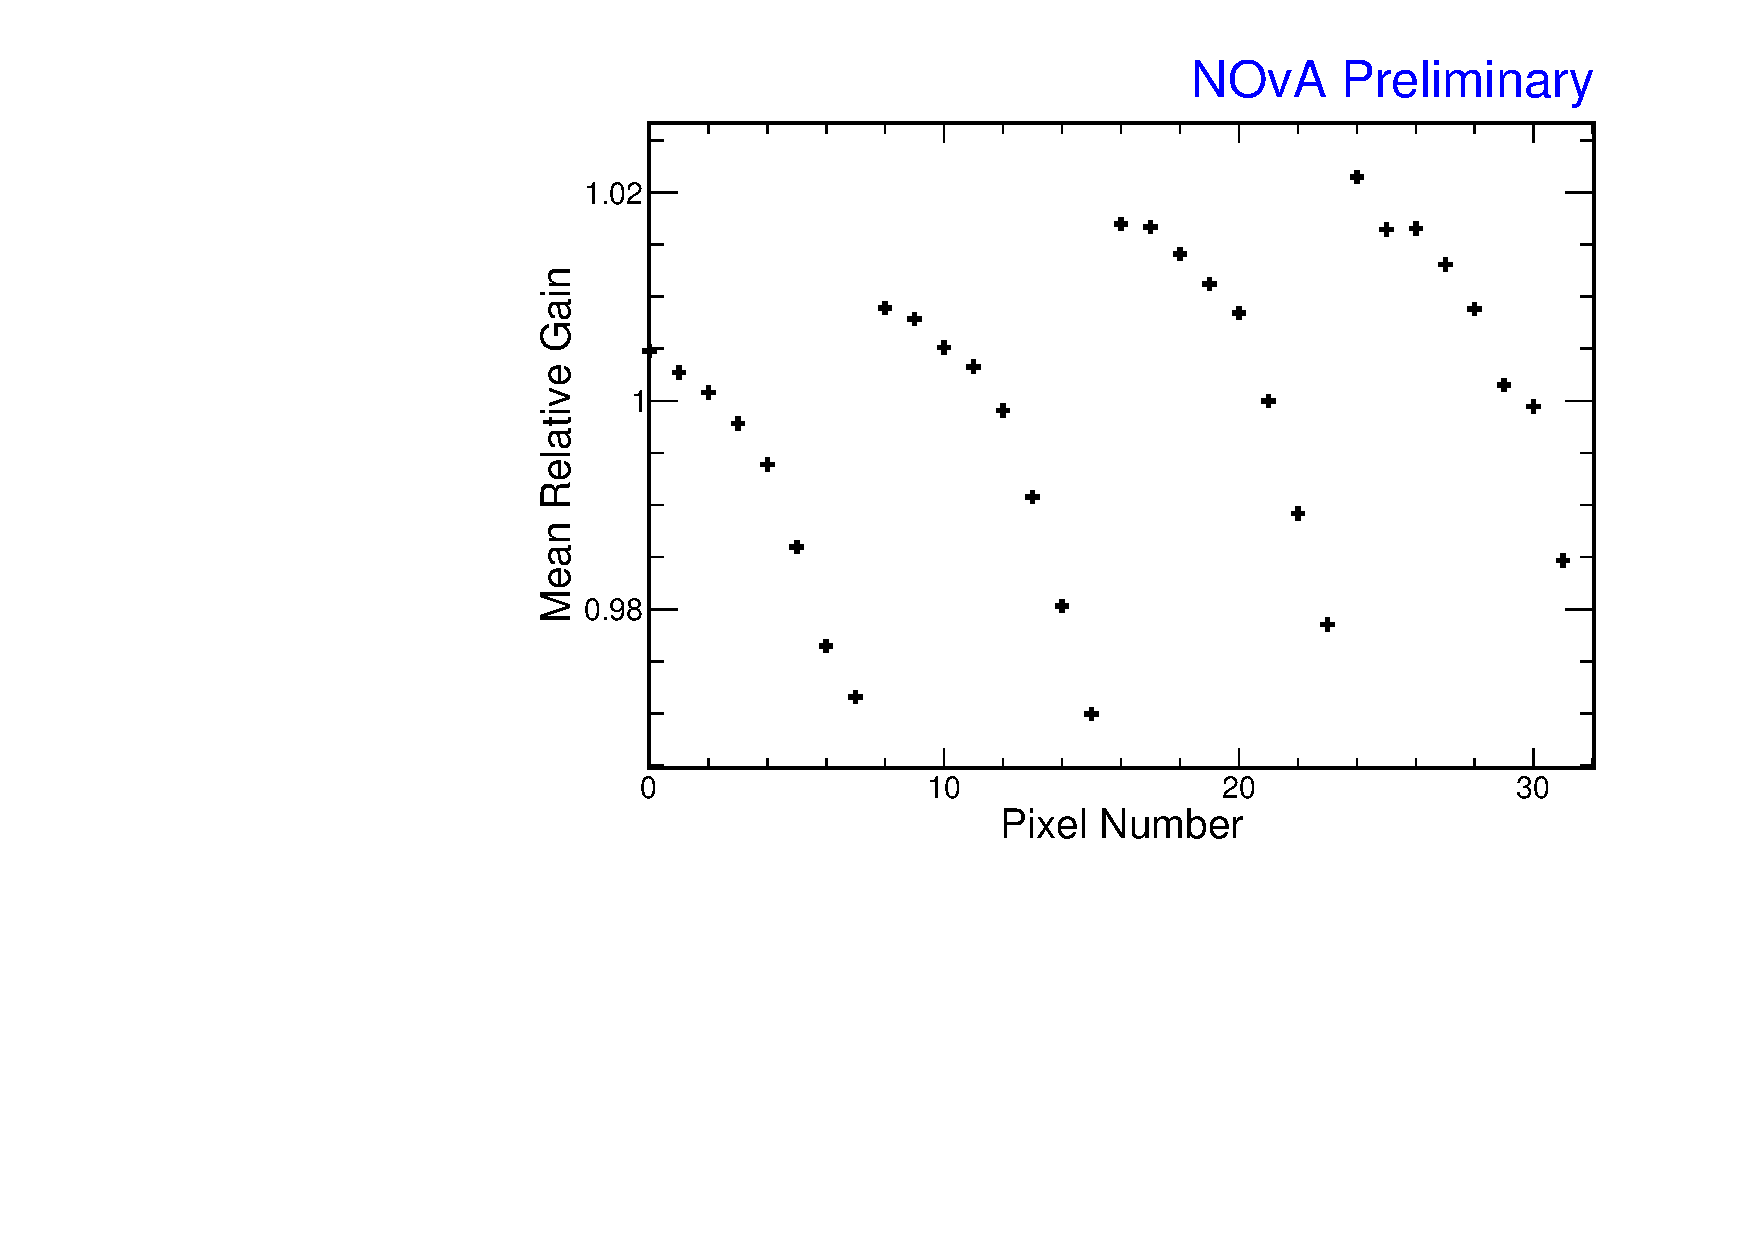
\includegraphics[width=\textwidth]{Plots/TBCalibration/ReadoutSimulation_GainPixelMap.pdf}
\end{subfigure}
\begin{subfigure}[t]{.495\textwidth}
\centering
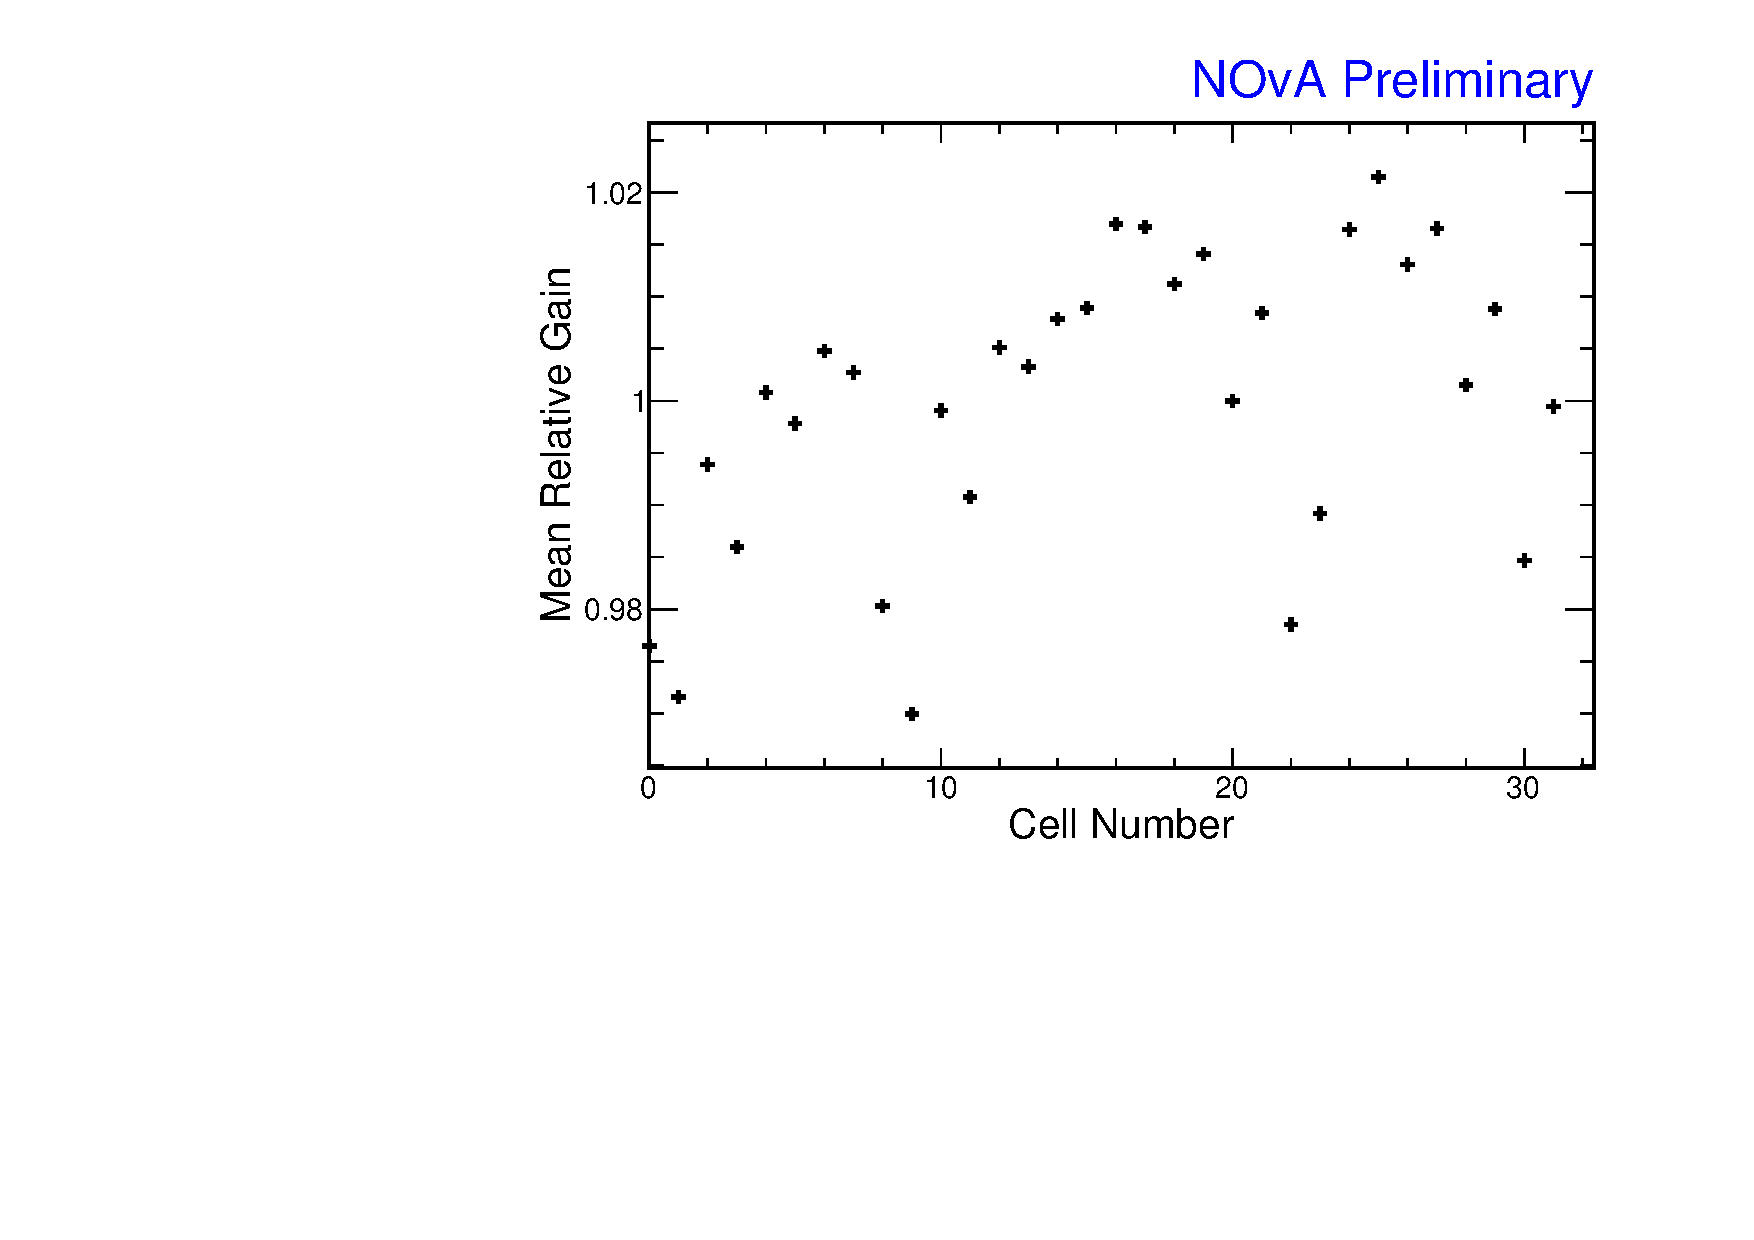
\includegraphics[width=\textwidth]{Plots/TBCalibration/ReadoutSimulation_GainCellMap.pdf}
\end{subfigure}
\caption{The relative gain variation as a function of the `pixel number' (left) and cell number (right).}
\label{fig:TBThresholdCorrectionGainMap}
\end{figure}

%Conclusion
In summary, the threshold and shielding correction exhibits significant variations concentrated within specific planes and cells, arising from various effects in the readout simulation. However, it is evident that these effects are not limited to cosmic events and therefore should not be incorporated into the threshold and shielding correction. Given that these effects are corrected out for simulation before the attenuation fits, they are not accounted for in the relative calibration and therefore remain present for the absolute calibration and for beam events. Moreover, the two main effects outline above are not implemented into the simulation correctly, resulting in discrepancies between actual data and simulation. This means, that in data these variations are either not present or present in a different way than in simulation. Therefore, applying the simulation-based threshold and shielding corrections to data introduces new variations that would otherwise not exist for data. As a result, these new variations are incorporated into the attenuation fits for data, resulting in incorrect relative calibration results applied to both absolute calibration and beam events.

%future, solutions
Several approaches can address these issues. For simulation-related discrepancies, the only viable solution is to rectify the identified faults and to remake the simulation, albeit this would be computationally very intensive. However, for data-related concerns, efforts are underway to devise a new data-driven threshold and shielding correction \cite{NOvA-doc-15223}, eliminating any influence of simulation on the relative calibration of data. If a purely data-driven correction is not viable, there is another possible improvement to the threshold correction while still using simulation, which is to not use the $\gls{PE}_{\mathrm{Poisson}\lambda}$ directly, but to pass it through the readout simulation in the same way as $\gls{PE}_{\mathrm{True}}$ and create an alternative $\gls{PE}_{\mathrm{Poisson}\lambda\mathrm{Reco}}$.

\section{Simulation}\label{sec:SimulationResults}
The distribution of tricell hits from the simulated cosmic muon events selected for calibration, mapped across the Test Beam detector's planes and cells, is shown in Fig.~\ref{fig:CalibhistSim}. As this is a simulated detector, we will use this `ideal conditions' distribution of tricell hits to illustrate the main features, which are also present in all the data samples discussed below. We can clearly see the difference in the number of events between the vertical (even) and the horizontal (odd) planes. This is expected as cosmic muons are generally vertical and a single cosmic track often passes more horizontal planes than vertical planes. We can also see that due to the tricell condition there are no hits in cells 0 and 63, which are on the edge of the detector. These cells can still be calibrated by including hits from the `z tricell' condition, which is not shown in the plot. The three clear horizontal lines of relatively lower response going across the detector correspond to pairs of cells 15 + 16, 31 + 32, and 47 + 48. Together with cells 0 and 63, they represent the first and the last cells of each 16 cell-wide extrusion, which makes up half of a module, which in turn makes up half of a Test Beam plane. As was mentioned in Sec.~\ref{sec:NOvADetectors}, these cells are $\unit[3]{mm}$ narrower than the rest, resulting in fewer hits and a lower deposited energy. However, using the deposited energy divided by path length for calibration should compensate for this effect. Overall, Fig.~\ref{fig:CalibhistSim} demonstrates that the tricell hits are distributed fairly uniformly in the centre of the detector, with the number of hits dropping off towards the front, back and corners of the detector. This is a result of the event selection applied to the cosmic tracks for calibration.

\begin{figure}[h]
\centering
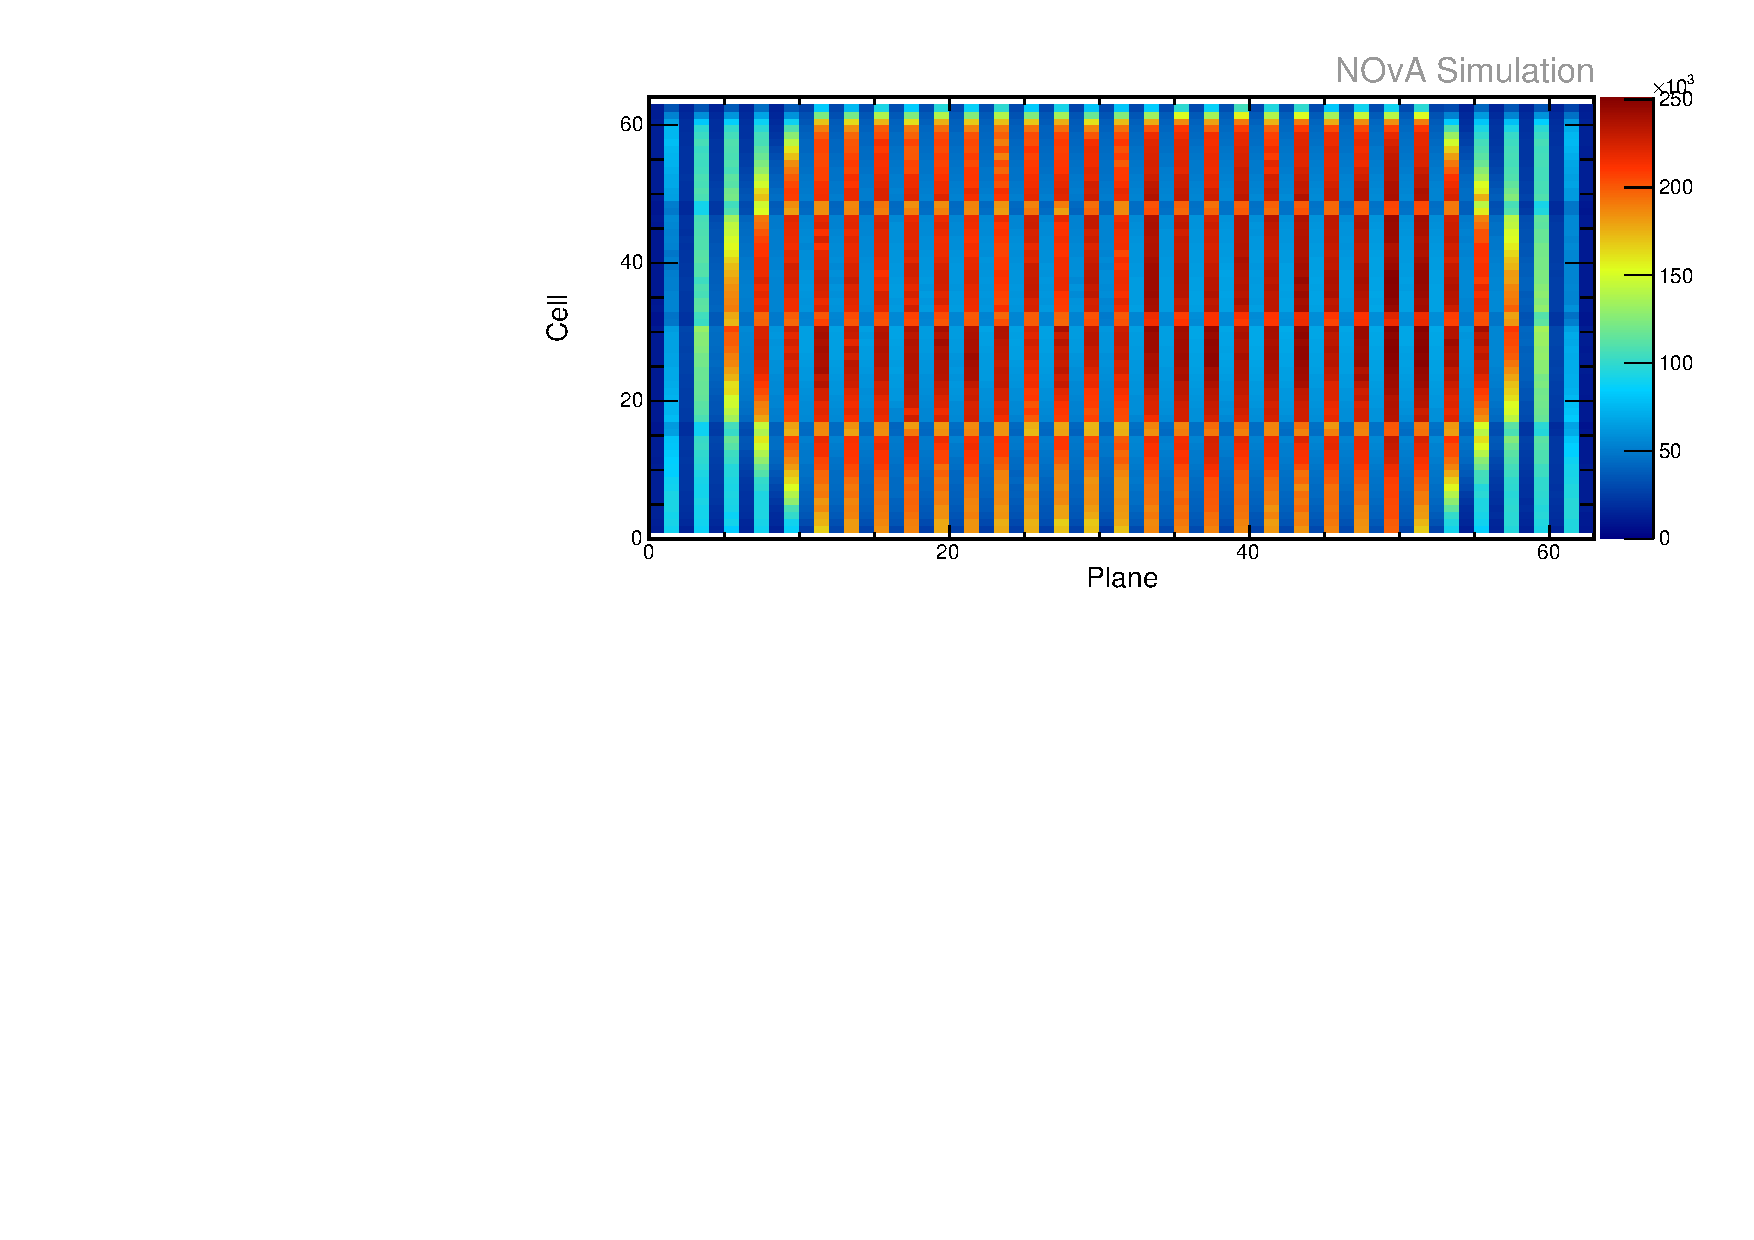
\includegraphics[width=\textwidth]{Plots/TBCalibration/Attenprofs_Simulation_CellPlane.pdf}
\caption[Plane-Cell distribution of hits for the simulation sample]{Distribution of tricell hits used for the calibration of the simulated Test Beam detector. Features are described in text.}
\label{fig:CalibhistSim}
\end{figure}

The distributions of deposited energy per path length though the cell before the calibration in units of $\unit{PE/cm}$ as a function of $w$, cell and plane number, are shown in Fig.~\ref{fig:Calibhist_simulation}. These distributions should be uniform after applying the results of the calibration and can be used to identify the main features that will need to be corrected for during the calibration. The shallow rise of the energy response along $w$ is caused by the attenuation of light along the \gls{WLS} fibres. The drop in the response at the edges of the cell is caused by the fibres looping and connecting to the \glspl{APD}, while the larger statistical uncertainties at the edges of the cell reflect the lower number of hits passing the event selection including the tricell condition.

\begin{figure}[h]
\centering
\begin{subfigure}[b]{0.495\textwidth}
\centering
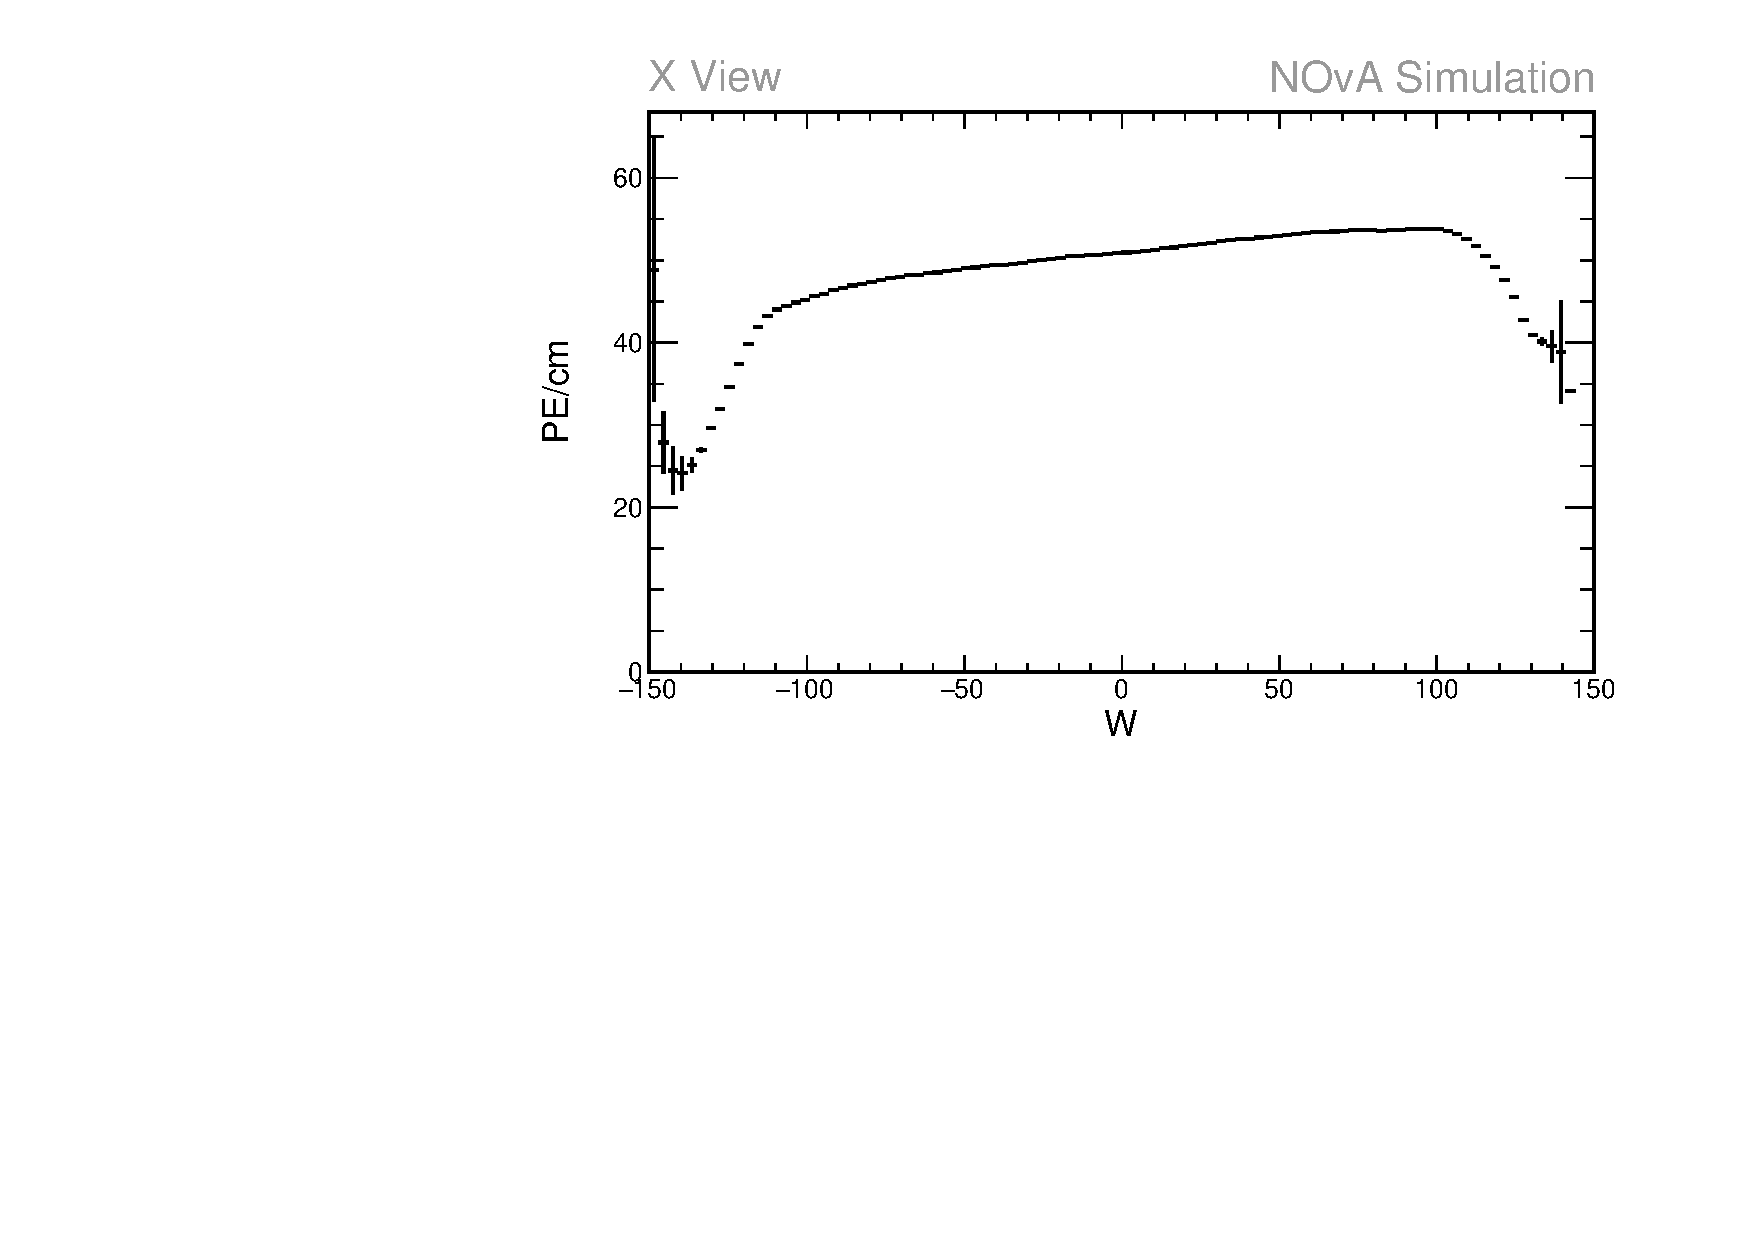
\includegraphics[width=\textwidth]{Plots/TBCalibration/Attenprofs_Simulation_WPE_corr_xy_X_Prof.pdf}
\end{subfigure}
\begin{subfigure}[b]{0.495\textwidth}
\centering
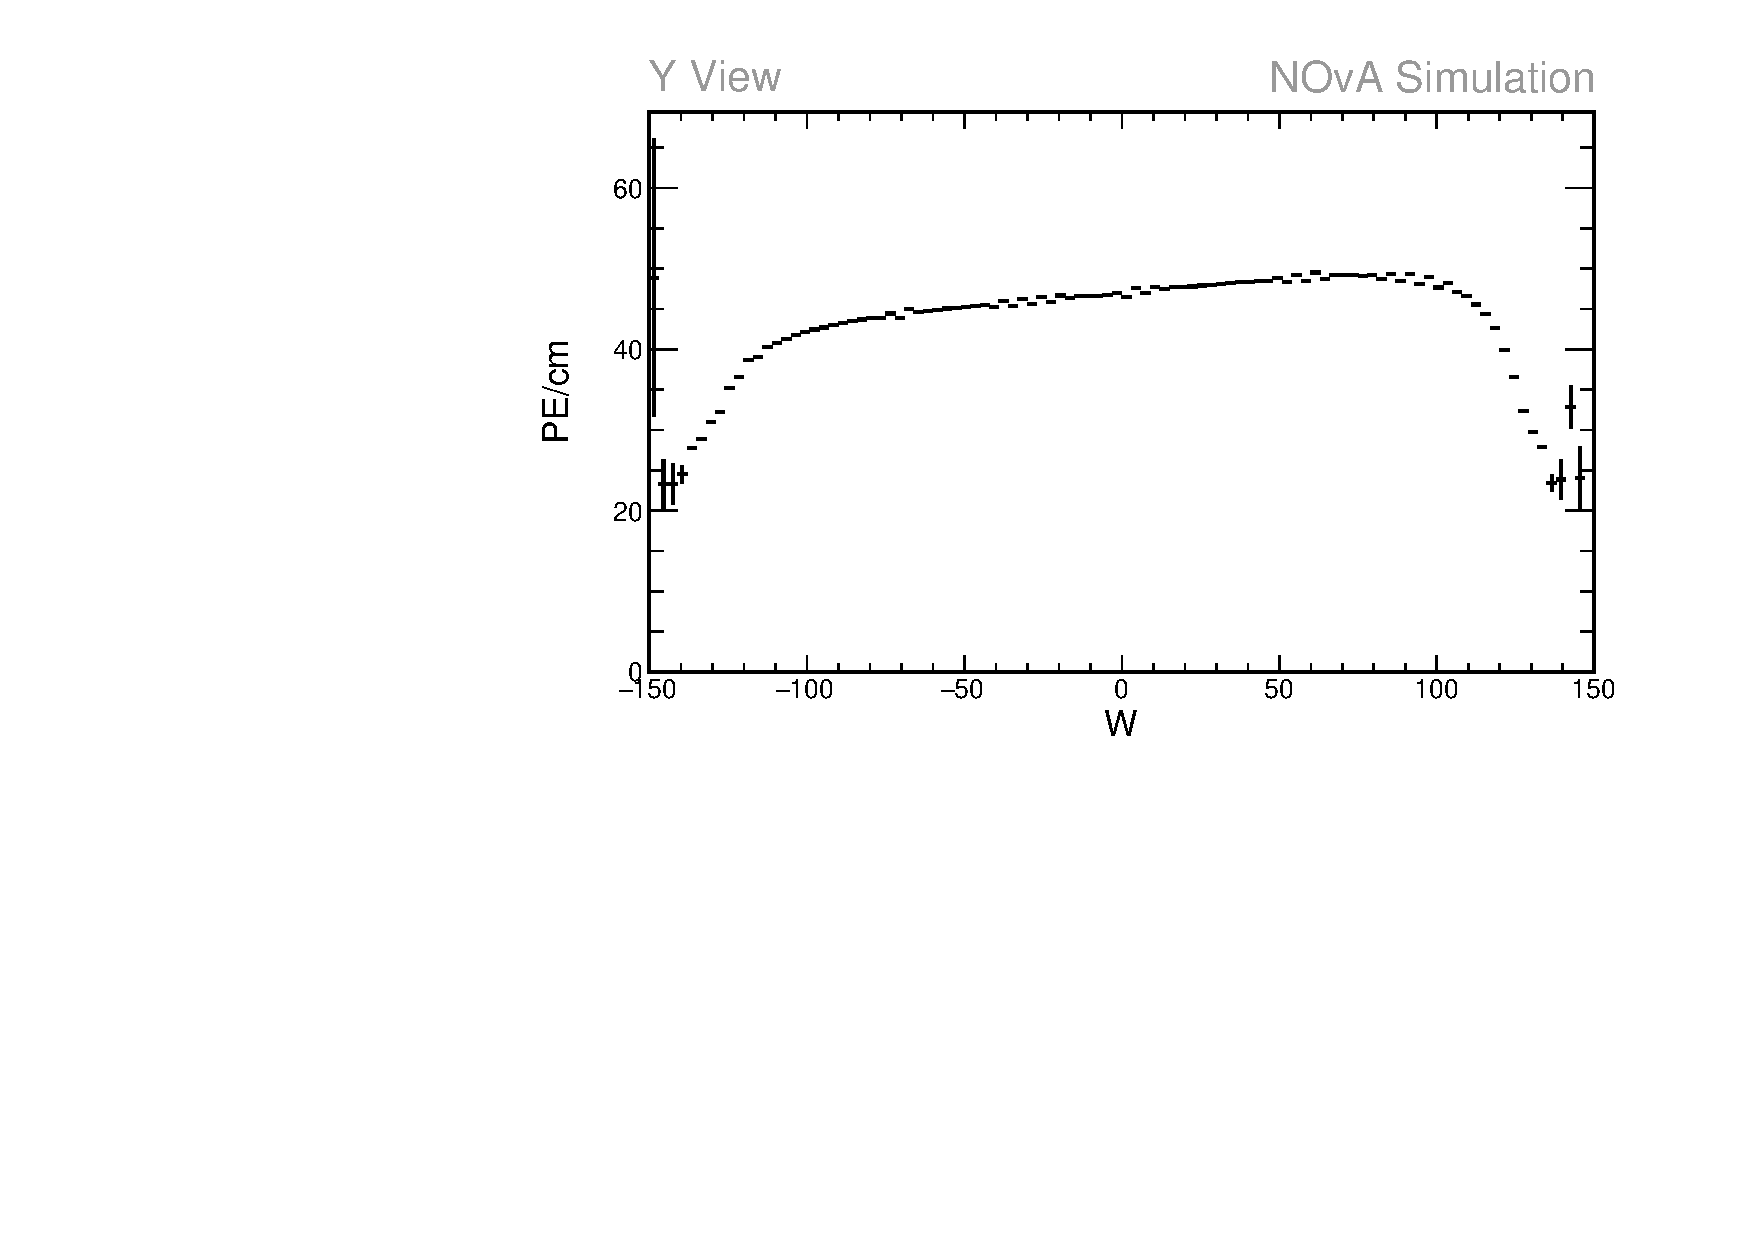
\includegraphics[width=\textwidth]{Plots/TBCalibration/Attenprofs_Simulation_WPE_corr_xy_Y_Prof.pdf}
\end{subfigure}
\begin{subfigure}[b]{0.495\textwidth}
\centering
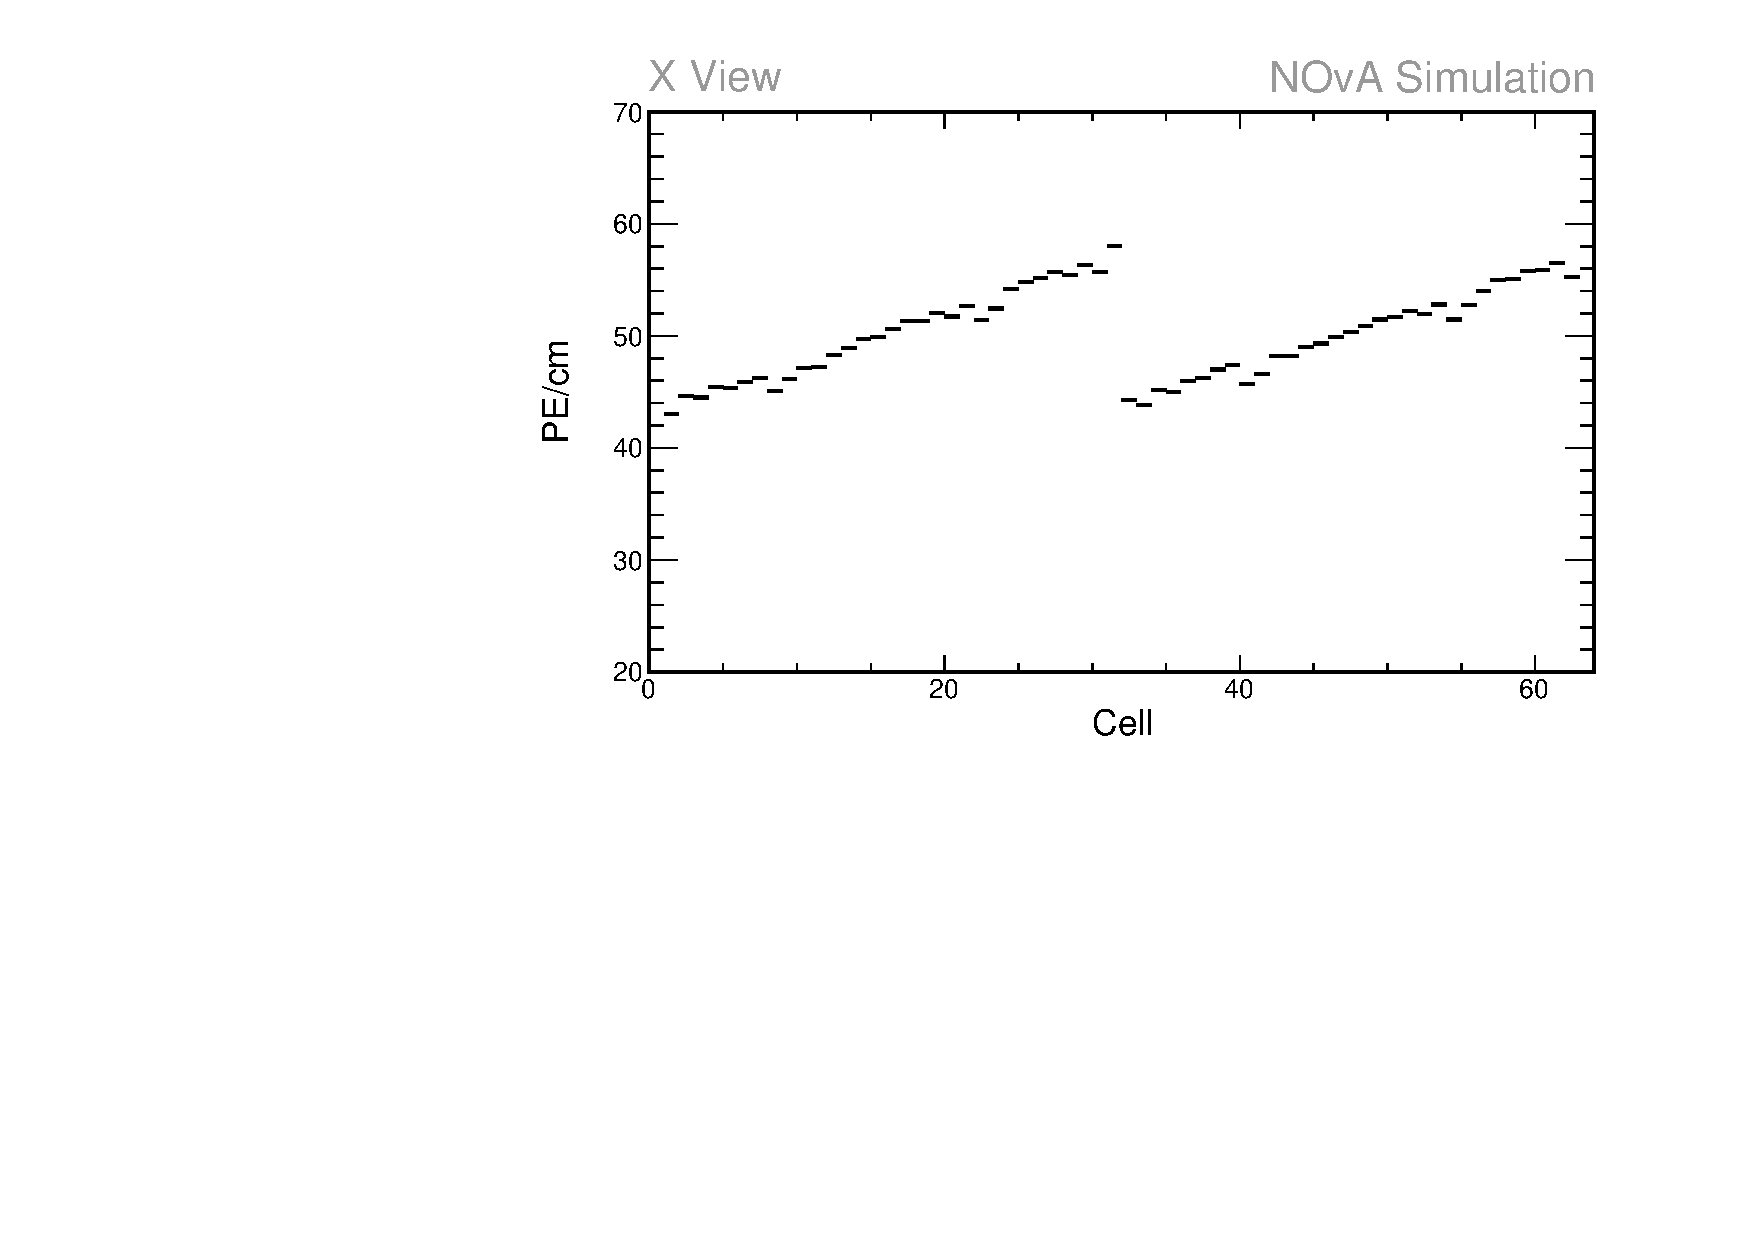
\includegraphics[width=\textwidth]{Plots/TBCalibration/Attenprofs_Simulation_CellPE_X_Prof.pdf}
\end{subfigure}
\begin{subfigure}[b]{0.495\textwidth}
\centering
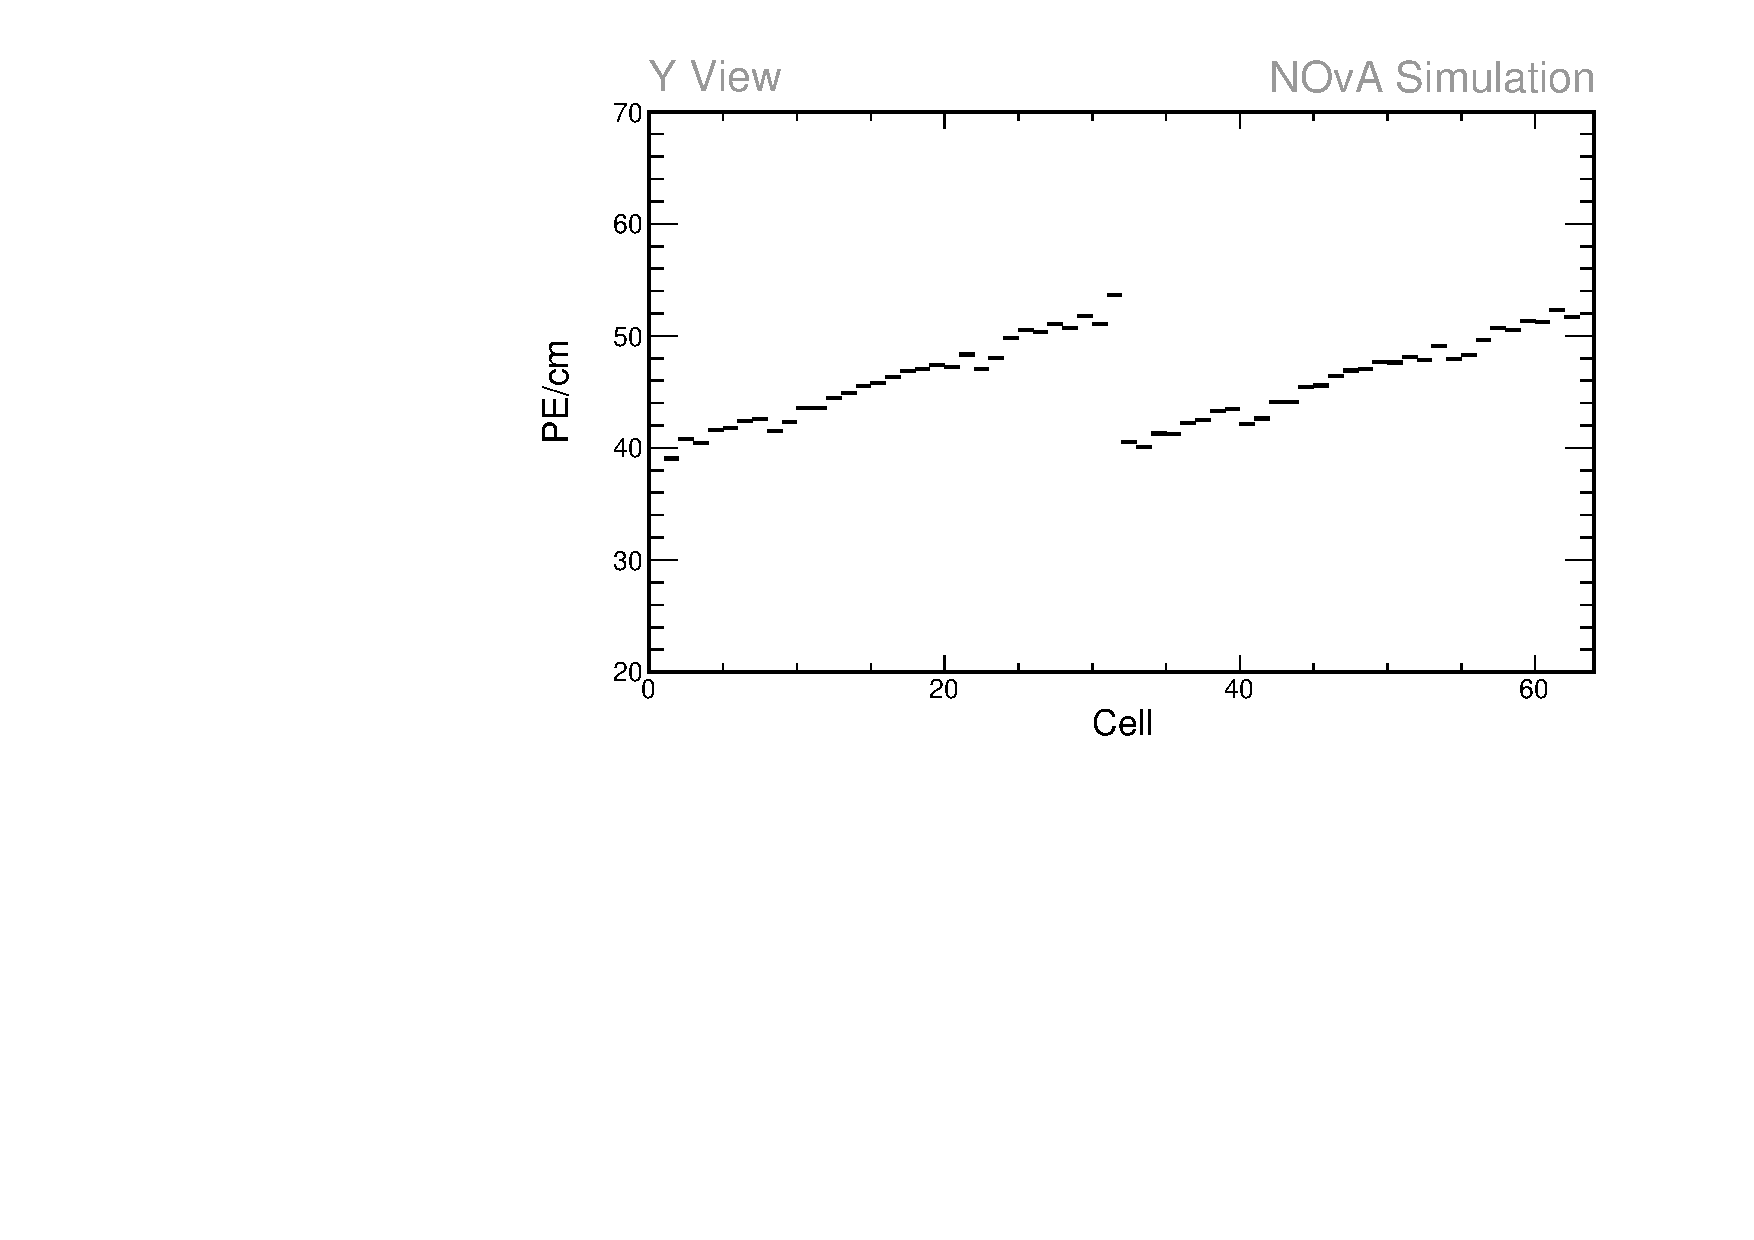
\includegraphics[width=\textwidth]{Plots/TBCalibration/Attenprofs_Simulation_CellPE_Y_Prof.pdf}
\end{subfigure}
\begin{subfigure}[b]{0.495\textwidth}
\centering
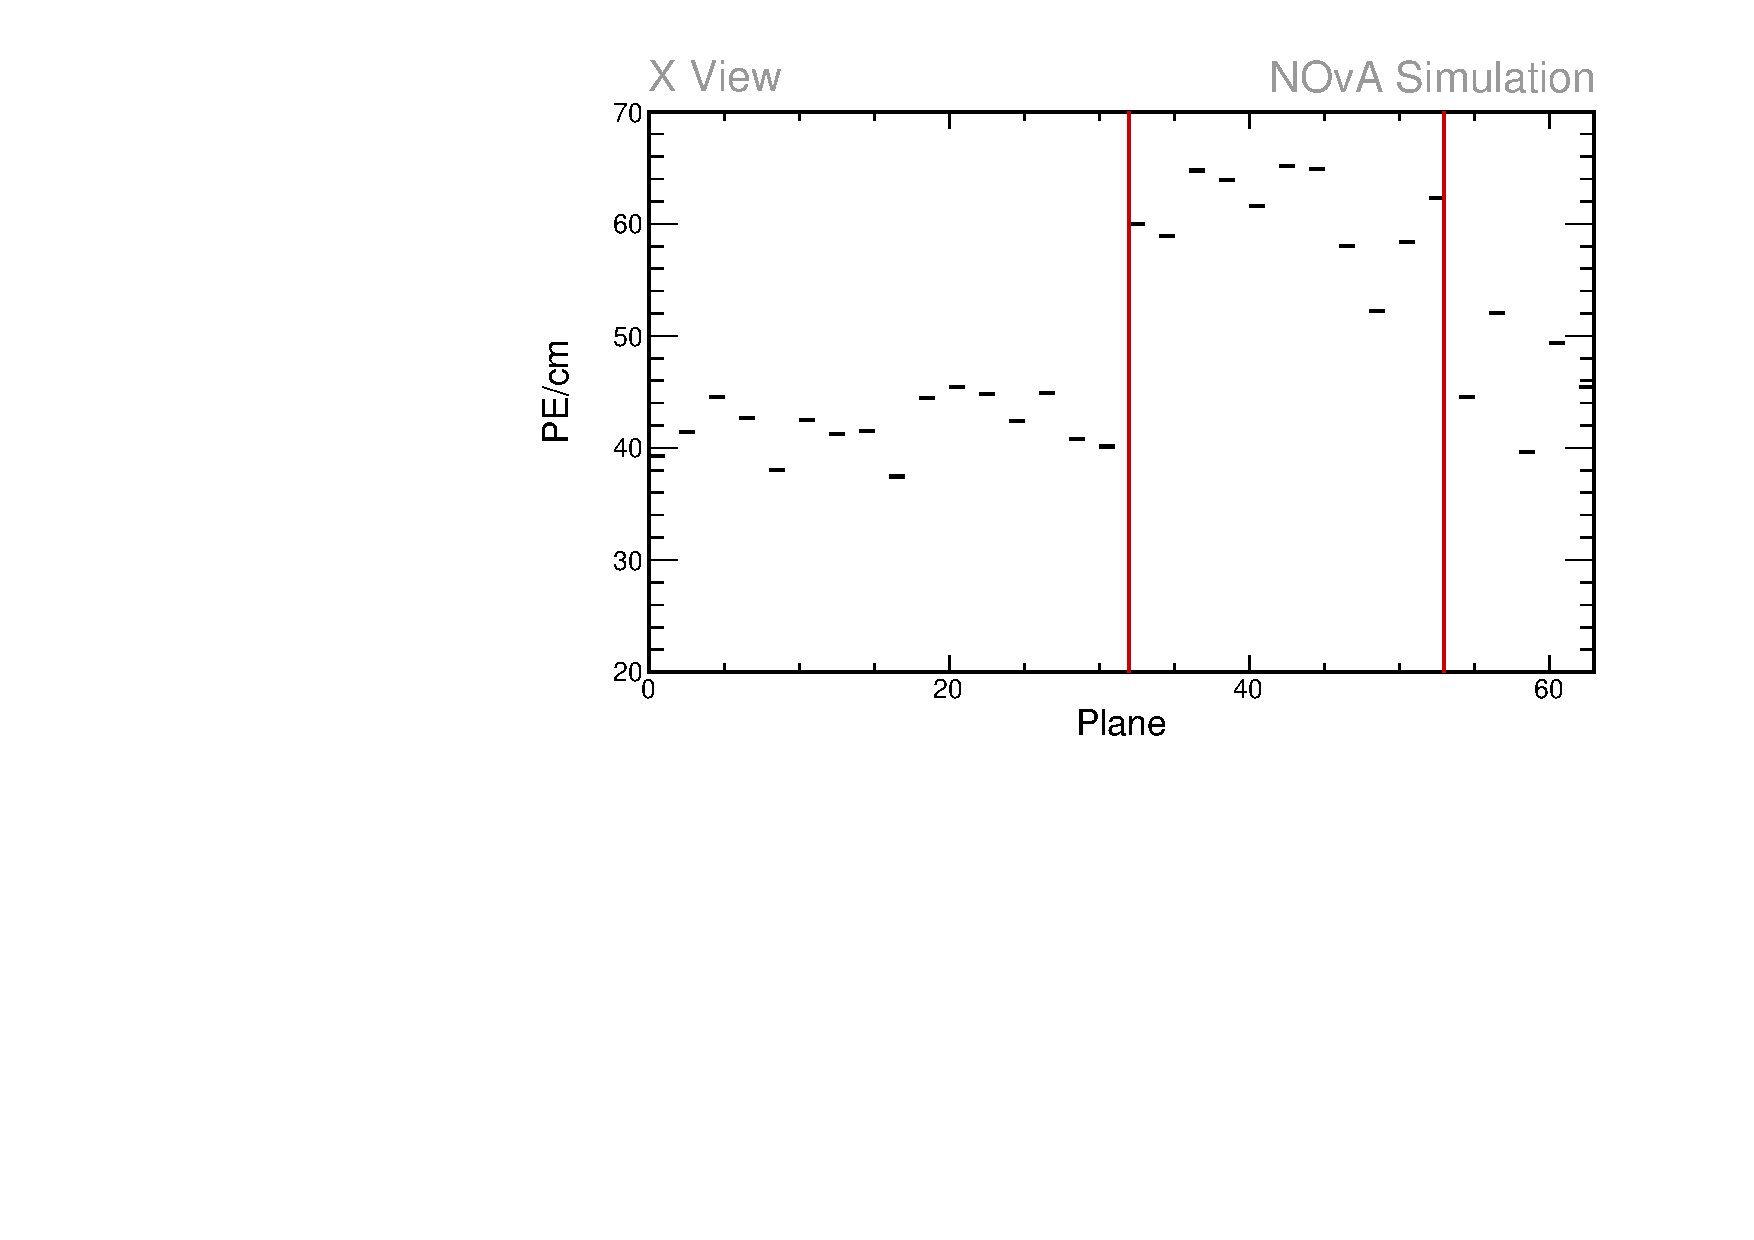
\includegraphics[width=\textwidth]{Plots/TBCalibration/Attenprofs_Simulation_PlanePE_X_Prof.pdf}
\end{subfigure}
\begin{subfigure}[b]{0.495\textwidth}
\centering
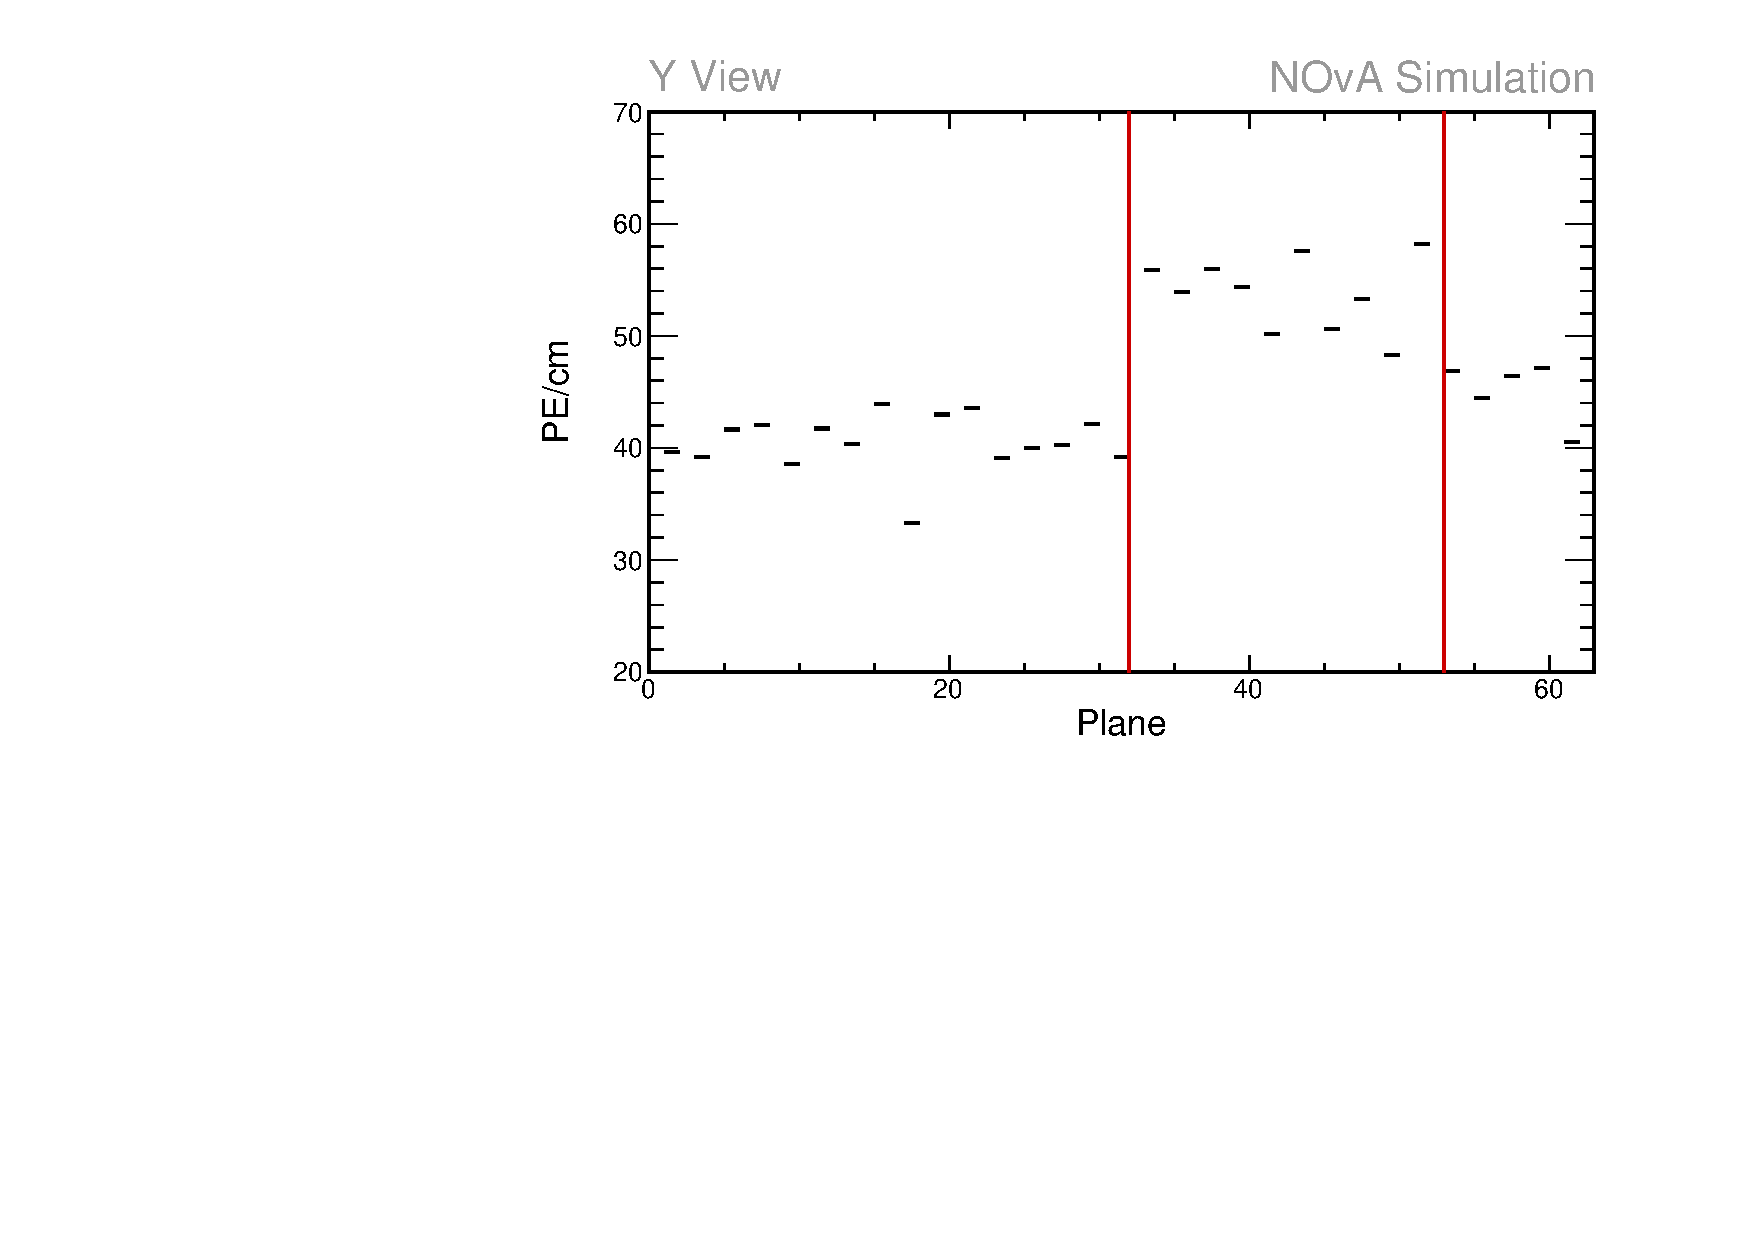
\includegraphics[width=\textwidth]{Plots/TBCalibration/Attenprofs_Simulation_PlanePE_Y_Prof.pdf}
\end{subfigure}
\caption[Uncorrected energy response along $w$, cell and plane for simulation]{Uncorrected average energy response as a function of the position within a cell ($w$ - top), cell number (middle), or plane number (bottom) for the Test Beam detector simulation of cosmic muon hits selected for calibration. Left side shows distributions for the X view (vertical) planes and right side for the Y view (horizontal) planes. Each plot is a profile histogram, with uncertainties representing statistical variations. Red lines on the bottom two plots depict the boundaries between different scintillators. Features explained in text.}
\label{fig:Calibhist_simulation}
\end{figure}

The rise of the response with the cell number, visible in the middle plots in Fig.~\ref{fig:Calibhist_simulation}, is due to the varying distance of cells to the readout. Since the \glspl{APD} are located on one side of each module, light from cells on the opposite side has to travel along the \gls{WLS} fibre for an additional module width, compared to the cells closer to the readout. Light undergoes additional attenuation along these so-called `pig tails', causing the difference of the energy response. The additional variations across cells within a module, notably the relatively lower response in cells 0, 1, 9, 10, 23, 24, 31 and 32, is caused by including the relative gain differences into the simulation, as explained above in Sec.~\ref{sec:TBThresholdCorrection}.

The uncorrected energy response as a function of plane number is shown in the bottom row of Fig.~\ref{fig:Calibhist_simulation}, illustrating large fluctuations between planes in both views. We can clearly identify the three distinctly different responses delineated by red lines, corresponding to the three scintillator variations used, as described in Sec.~\ref{sec:TBExperiment}. Additionally, planes 16, 17, 48 and 49 use the \gls{FEB}v5.2 instead of \gls{FEB}v4.1, resulting in a relatively lower response. All these variations between planes in simulation are caused by consolidating the planes and replacing possible discrepancies with the \gls{FB} map (Sec.~\ref{sec:FibreBrightnessTB}), which is used for simulation to emulate real detector conditions. The rest of the variations are caused by differences between readout electronics and individual cells, but are exacerbated by the \gls{FB} binning, which groups otherwise smooth variations across planes into 12 discrete bins, thus amplifying them.

\subsection*{Simulation relative calibration results}

An overview of the attenuation fit results for simulation is shown in Fig.~\ref{fig:CellCentreResponseSim} as a map of average fitted response in the centre of each cell. Blank cells mark the uncalibrated cells which failed the calibration condition (attenuation fit $\chi^2>0.2$). All the uncalibrated cells but one are on the edges of the detector, which is expected, as they have much fewer events that pass the calibration sample selection. There are 43 uncalibrated cells out of the total 4032 cells in the Test Beam detector, resulting in 1.07\% of the simulated detector remaining uncalibrated.

\begin{figure}[h]
\centering
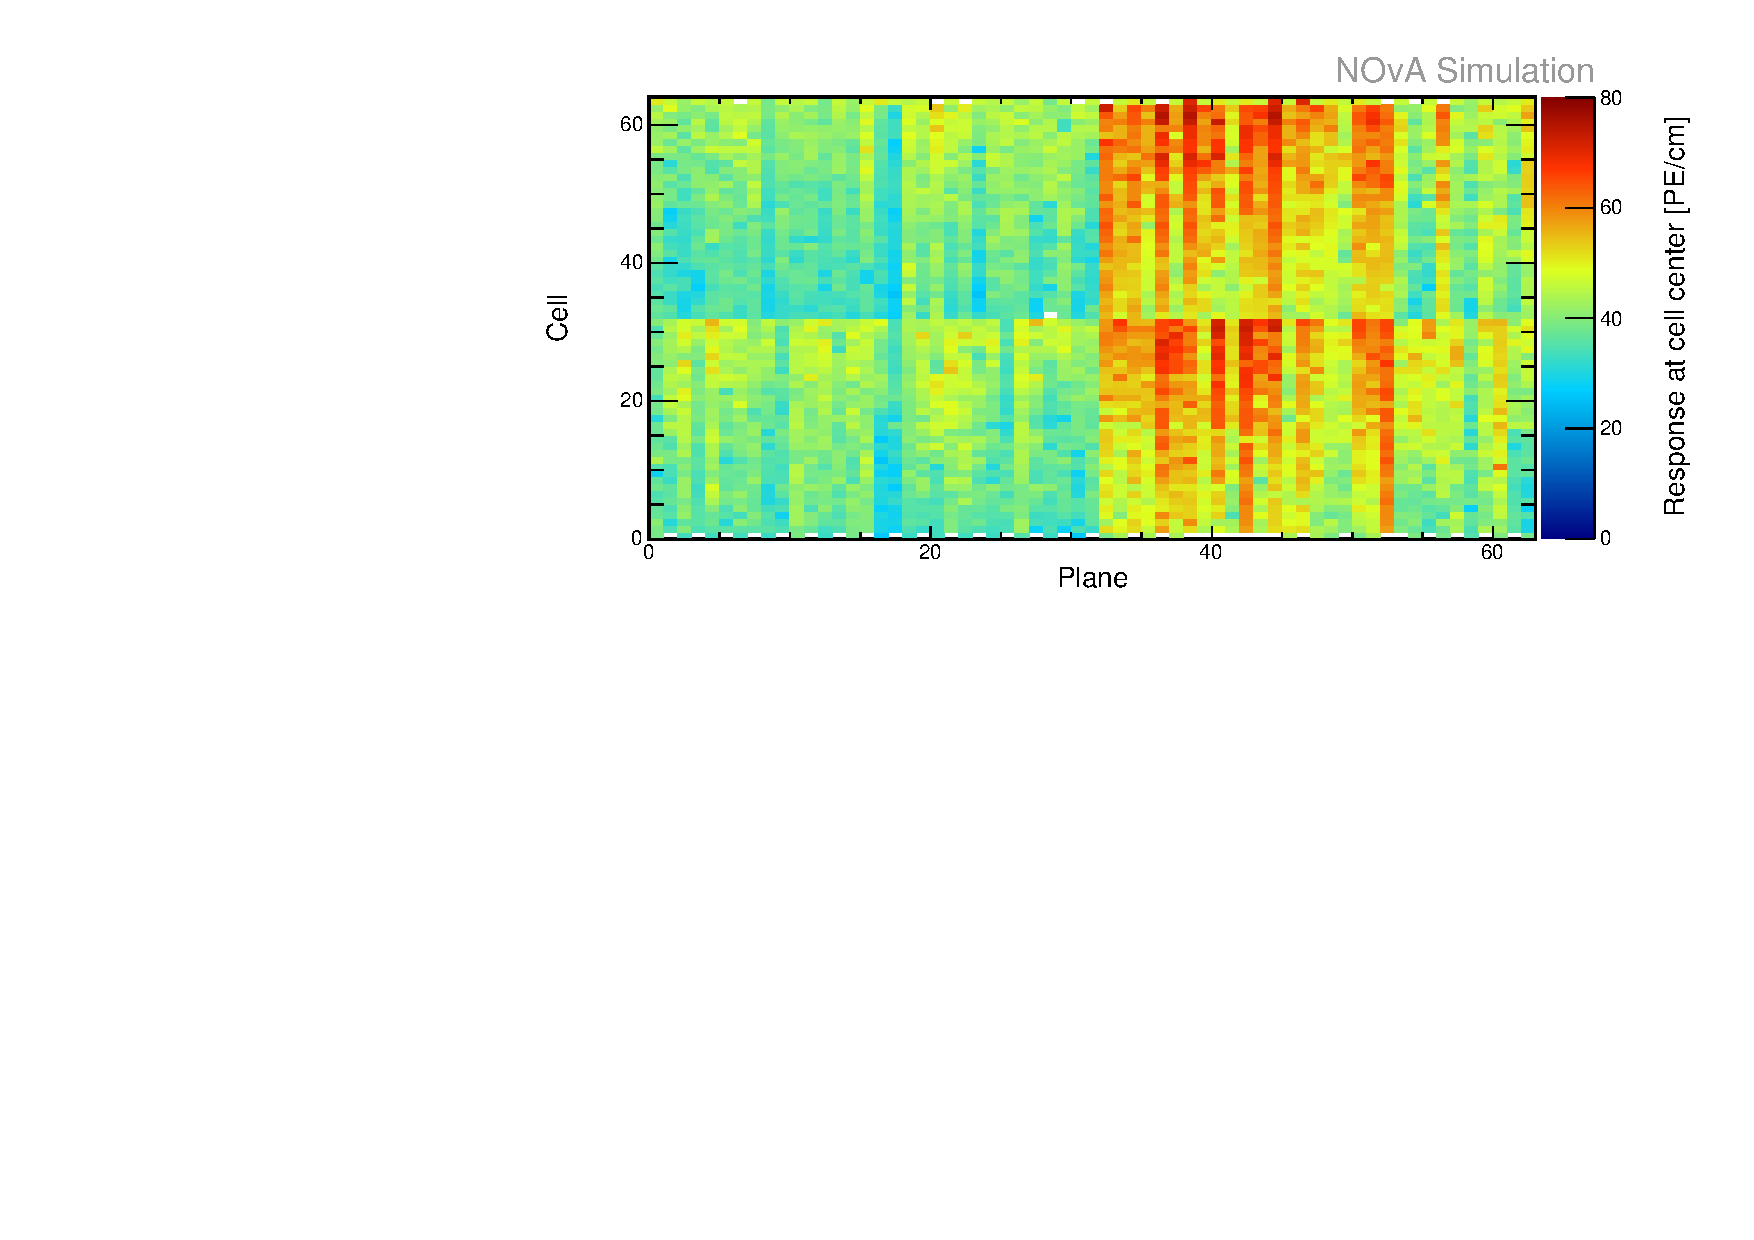
\includegraphics[width=\textwidth]{Plots/TBCalibration/CellResponseAtCentre_Prod4DataBasedSim_Limited_NOvAPlotStyle.pdf}
\caption[Map of fitted response at cell centre for simulation]{Overview of the attenuation fit results for the simulated Test Beam detector. Each cell represents the result of the attenuation fit to the energy response in the centre of that cell. The blank cells are uncalibrated as the attenuation fit did not satisfy the calibration condition.}
\label{fig:CellCentreResponseSim}
\end{figure}

For simulation, the attenuation fit is done for each \gls{FB} bin and each cell separately. Examples of detector response for different cells in various \gls{FB} bins are shown in Fig.~\ref{fig:AttenfitResultsSimulation}. Here the red line shows the initial exponential fit and the blue line depicts the final attenuation fit after the \gls{LOWESS} correction, as described in Sec.~\ref{sec:NOvACalibration}. The cells on the edge of the detector failed the calibration conditions due to the low number of entries causing large fluctuation in the mean response.

There is only one cell in the middle of the detector that is left uncalibrated. This is the cell 32 in a vertical plane in \gls{FB} bin 5, shown on the top right of Fig.~\ref{fig:AttenfitResultsSimulation}, with $\chi^2=0.227$. Apparently, the reason the attenuation fit for this cell failed the calibration condition is the unusually high response with a large uncertainty in the right-most bin. It is unclear why this bin has such an elevated mean response, but since this only causes an issue for a single cell, we decided to ignore it and leave it uncalibrated.

\begin{figure}[h]
  \begin{subfigure}{0.495\textwidth}
    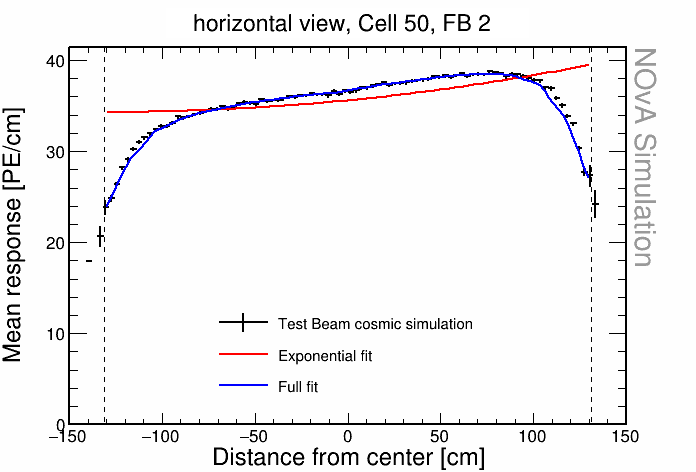
\includegraphics[width=\linewidth]{Plots/RelativeCalibrationResults/sim_fb2_001_050.png}
  \end{subfigure}
  \begin{subfigure}{0.495\textwidth}
    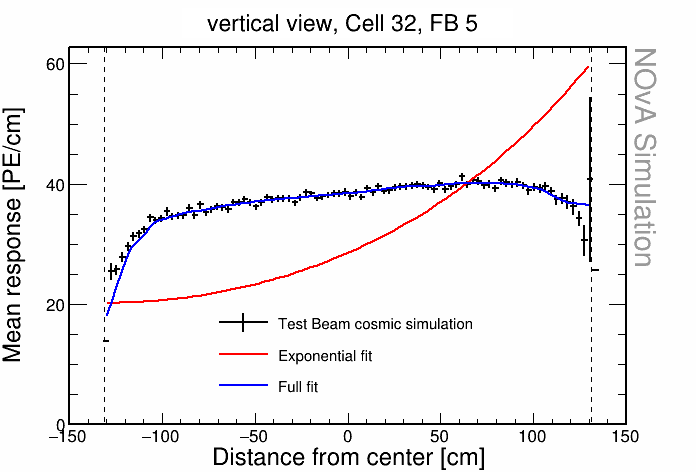
\includegraphics[width=\linewidth]{Plots/RelativeCalibrationResults/sim_fb5_000_032.png}
  \end{subfigure}
  \begin{subfigure}{0.495\textwidth}
    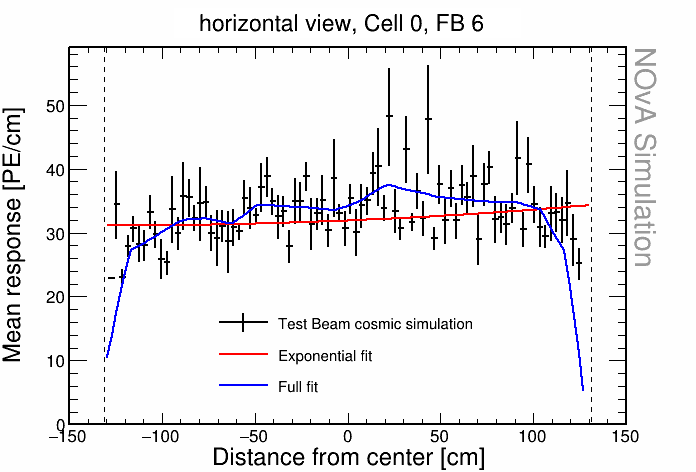
\includegraphics[width=\linewidth]{Plots/RelativeCalibrationResults/sim_fb6_001_000.png}
  \end{subfigure}
  \begin{subfigure}{0.495\textwidth}
    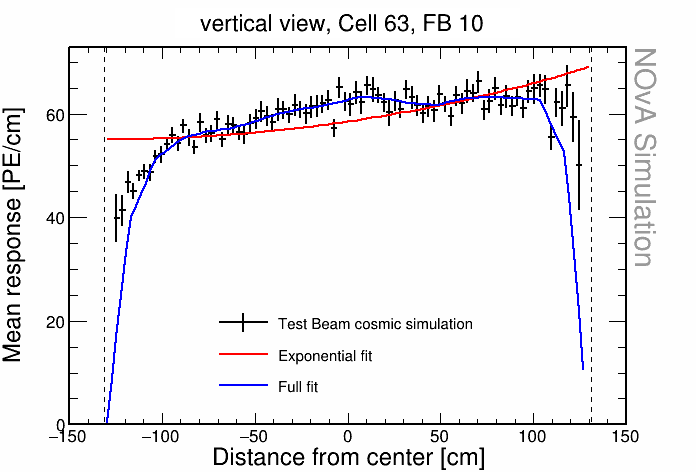
\includegraphics[width=\linewidth]{Plots/RelativeCalibrationResults/sim_fb10_000_063.png}
  \end{subfigure}
  \caption[Example attenuation fits for simulation]{Attenuation fits for a selection of cells in various \acrshort{FB} bins in the calibration of the Test Beam simulation. Top left is an example of a successful attenuation fit, top right is a failed fit due to statistical fluctuation in the last bin and the bottom plots show failed fits for cells on the edges of the detector.}
  \label{fig:AttenfitResultsSimulation}
\end{figure}

\section{Period 2 data}\label{sec:TBPeriod2}
The distribution of cosmic muon tricell hits selected for calibration in Test Beam period 2 data is shown in Fig.~\ref{fig:CalibhistMap_period2}.
The issue with underfilled cells described in Sec.~\ref{sec:TBExperiment} was present throughout period 2. The underfilled cells were marked as bad channels and therefore ignored during production of calibration samples. This also visibly affects the event count in the neighbouring cells to the underfilled cells, which have fewer calibration hits due to the tricell condition (see Sec.~\ref{sec:NOvACalibration}). However, since the underfilled cells 63 are also on the edge of the detector, labelling them as bad channels can't mitigate the effect on the neighbouring cells 62.

\begin{figure}[h]
\centering
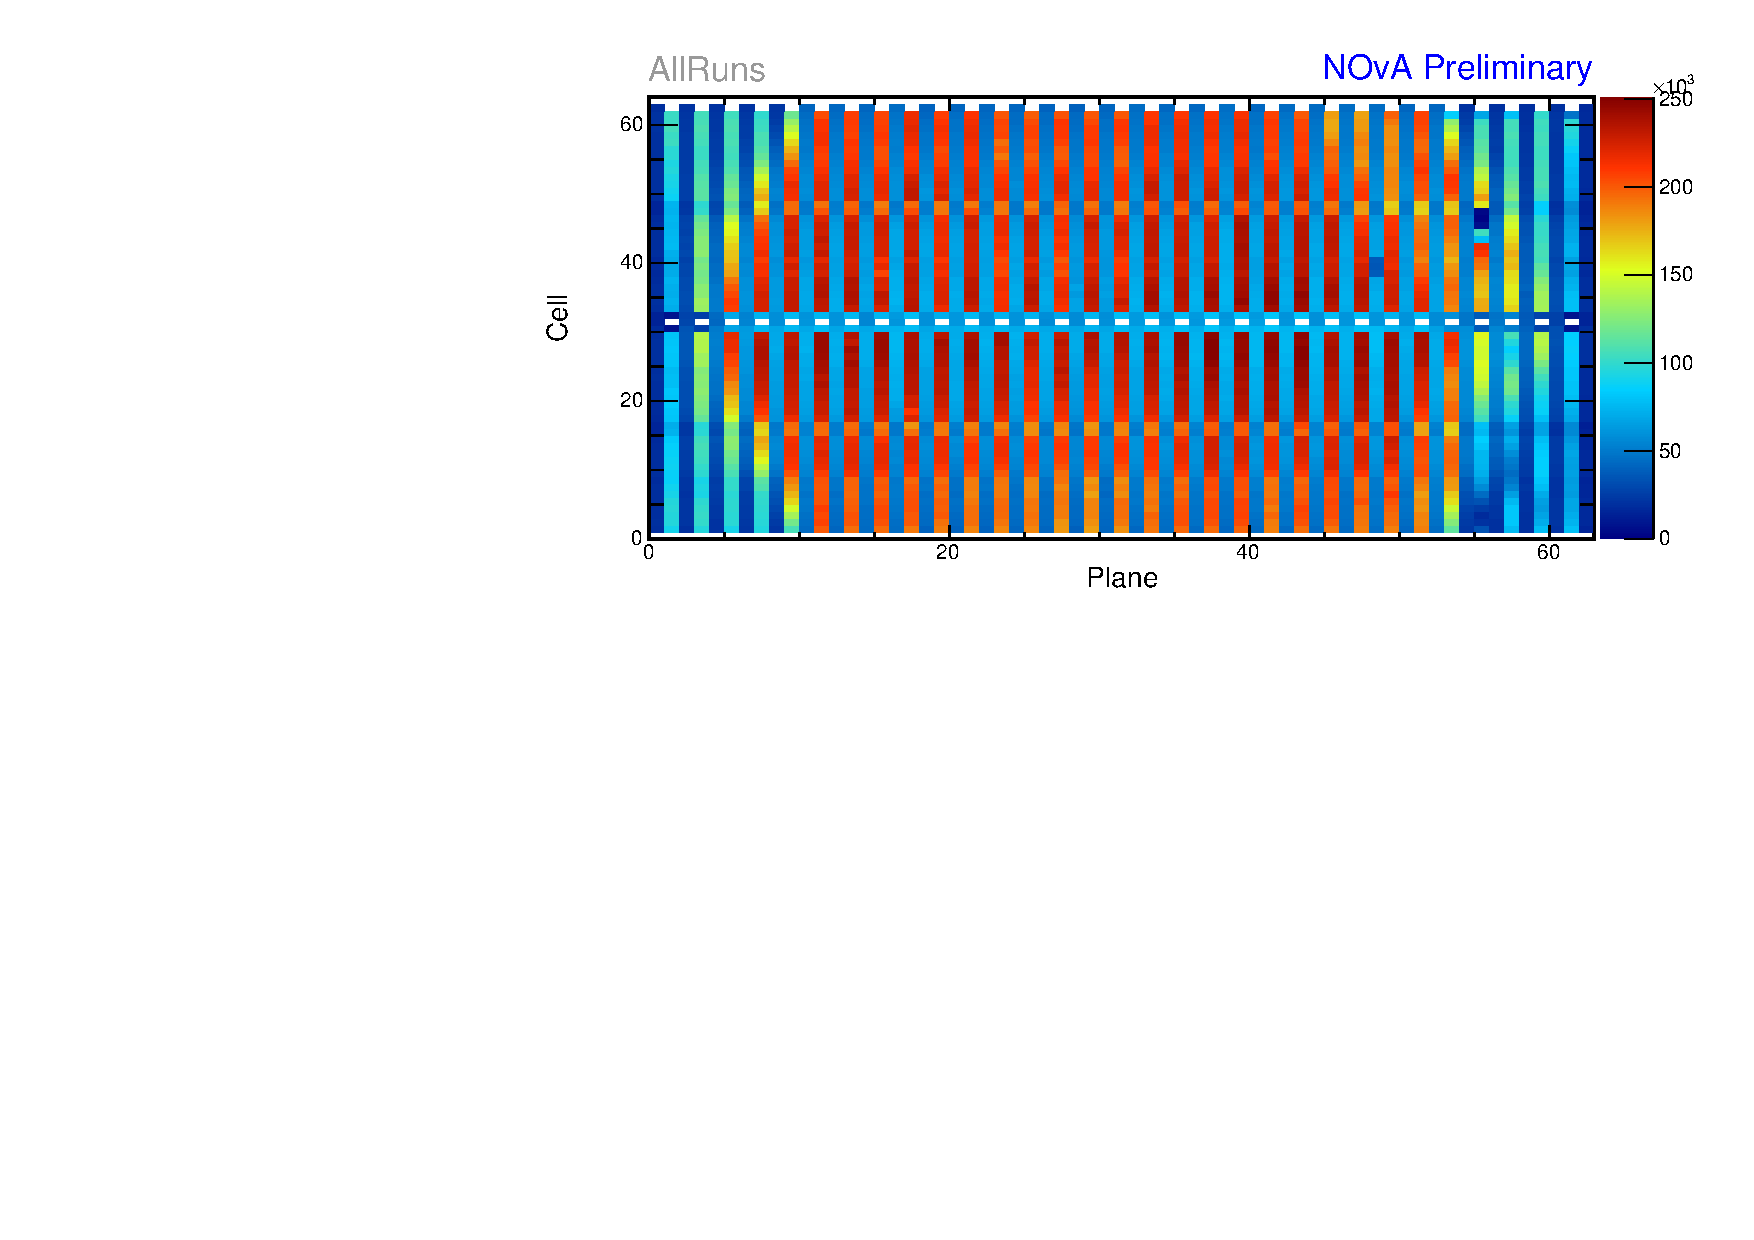
\includegraphics[width=\textwidth]{Plots/TBCalibration/Attenprofs_P2Data_CellPlane_AllRuns.pdf}
\caption[Plane-Cell distribution of tricell hits for period 2 data]{Distribution of tricell hits as a function of Test Beam detector cells and planes in the entire period 2 data calibration sample. The rows of empty cells 31 and 62 across all the horizontal planes are caused by the underfilled cells (and tricell condition), as explained in text. There are several areas with relatively fewer hits. Notably cells 38-40 in plane 48 and cells 45-47 in plane 55. Both of these spots comprise of three cells, pointing towards the middle cell being a dead channel (for a limited time) and the two surrounding cells being affected by the tricell condition. Additionally, the bottom half of planes 55 and 57 have noticeably lower number of hits than their top halves (one half corresponds to a single readout).}
\label{fig:CalibhistMap_period2}
\end{figure}

We can also observe areas with relatively fewer hits, likely due to channels that were dead for some time. This also affects their immediate neighbours due to the tricell condition. Additionally, there are planes that have noticeably fewer hits in one half than in the other, and since half of a plane corresponds to a single readout (one \gls{FEB} and \gls{APD}), which means an entire readout was faulty for a certain time.

Officially, period 2 is divided into six epochs labelled 2a - 2f, based on specific Test Beam detector running conditions. Generally, smaller calibration samples reduce time-dependent effects on calibration, such as detector ageing or temperature and humidity variations. However, smaller samples also increase the number of cells with issues in the attenuation fit (examples shown below). Therefore, it is important to choose an optimal calibration sample size to balance both concerns. Since individual epochs in period 2 do not contain enough events for a successful attenuation fit, and variations between epochs are minimal, we decided to calibrate the entire period 2 together, without splitting it into any smaller calibration samples.

The epochs in period 2 mostly differ in the use of various \gls{FEB} firmwares or in the presence of trigger studies. We compare the energy deposition during the individual epochs in Fig.~\ref{fig:Calibhist_period2}. As can be seen, the difference between the energy response across the individual epochs is fairly small (within $\unit[2]{\%}$) and only in normalization, with the largest outliers seemingly epochs 2a and 2d. There is also no clear trend of energy response falling or raising with time (epoch labels are organized in time alphabetically).

\begin{figure}[!hbtp]
\centering
\begin{subfigure}[b]{0.495\textwidth}
\centering
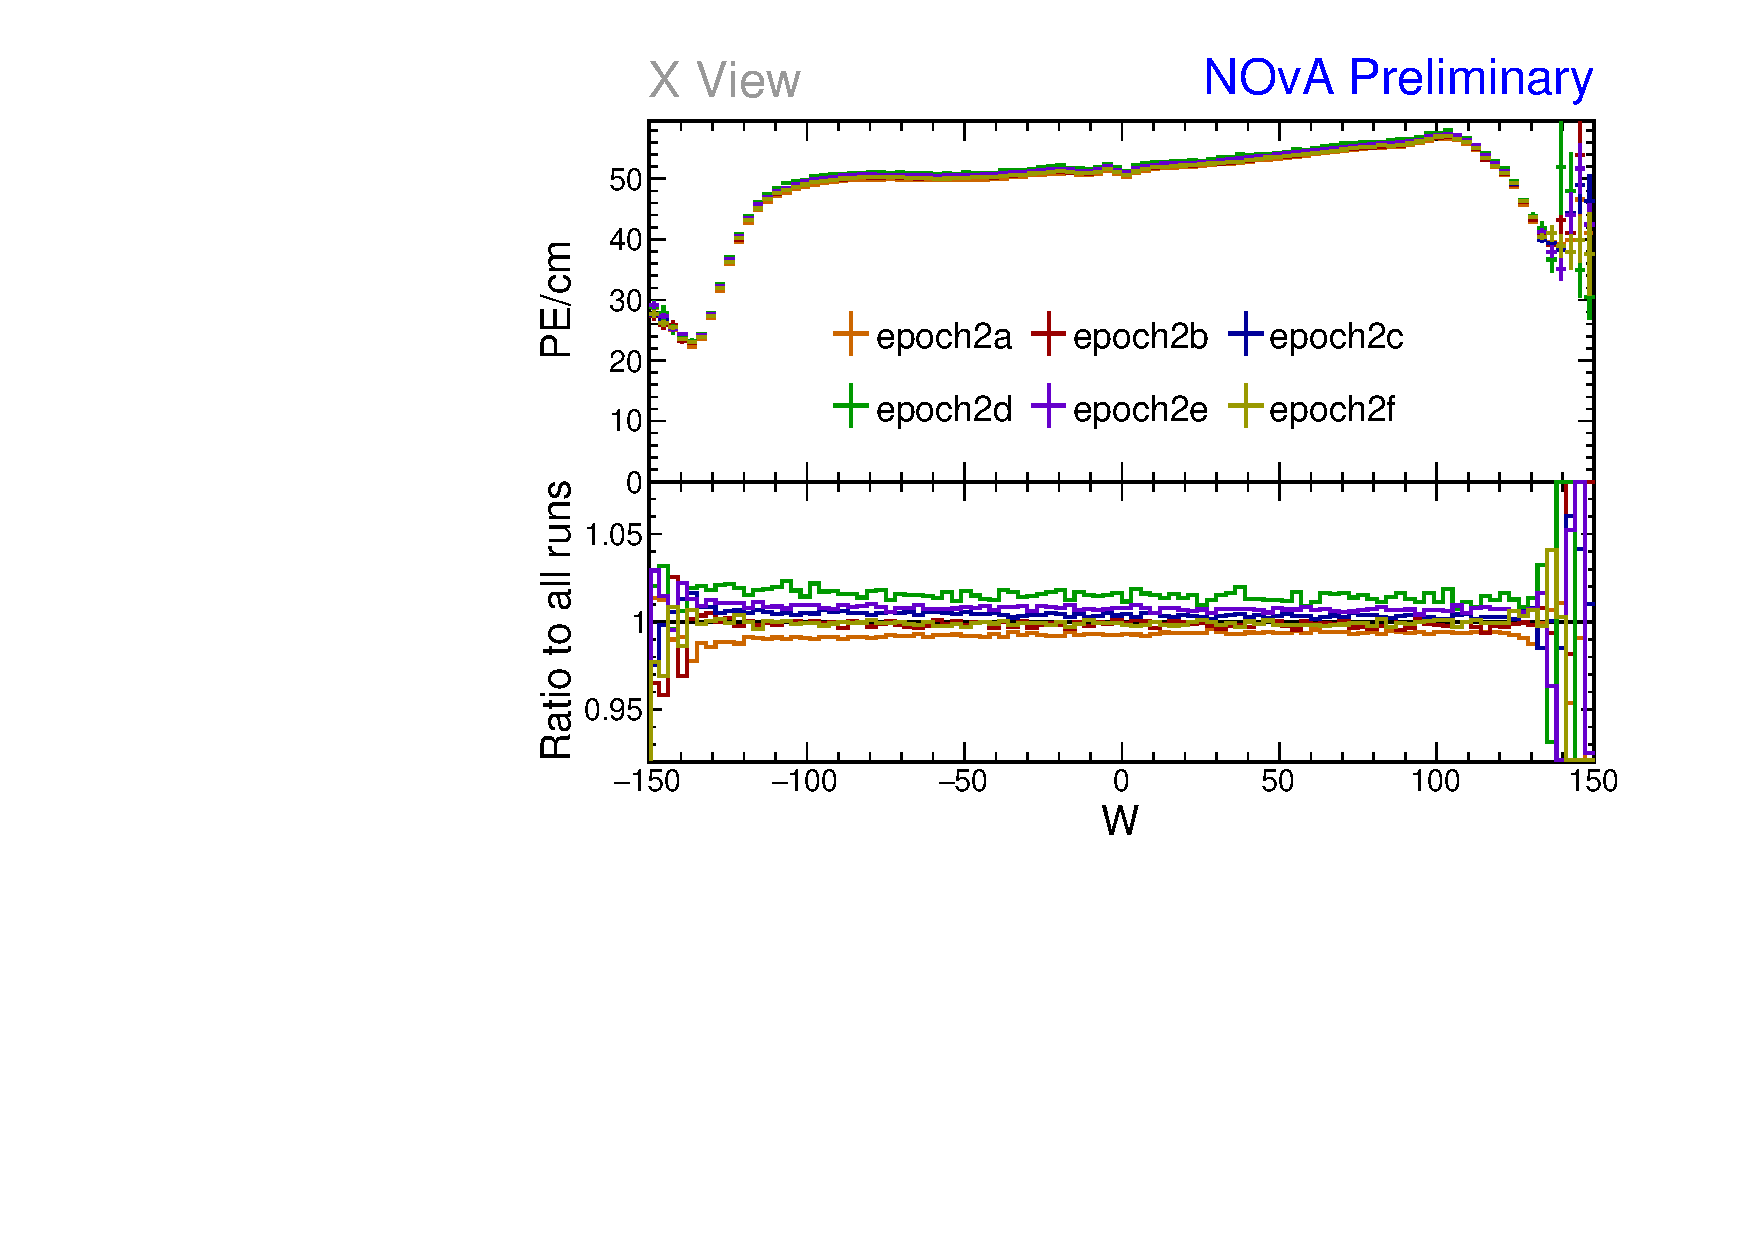
\includegraphics[width=\textwidth]{Plots/TBCalibration/Attenprofs_P2Data_WPE_corr_xy_X_Combined.pdf}
\end{subfigure}
\begin{subfigure}[b]{0.495\textwidth}
\centering
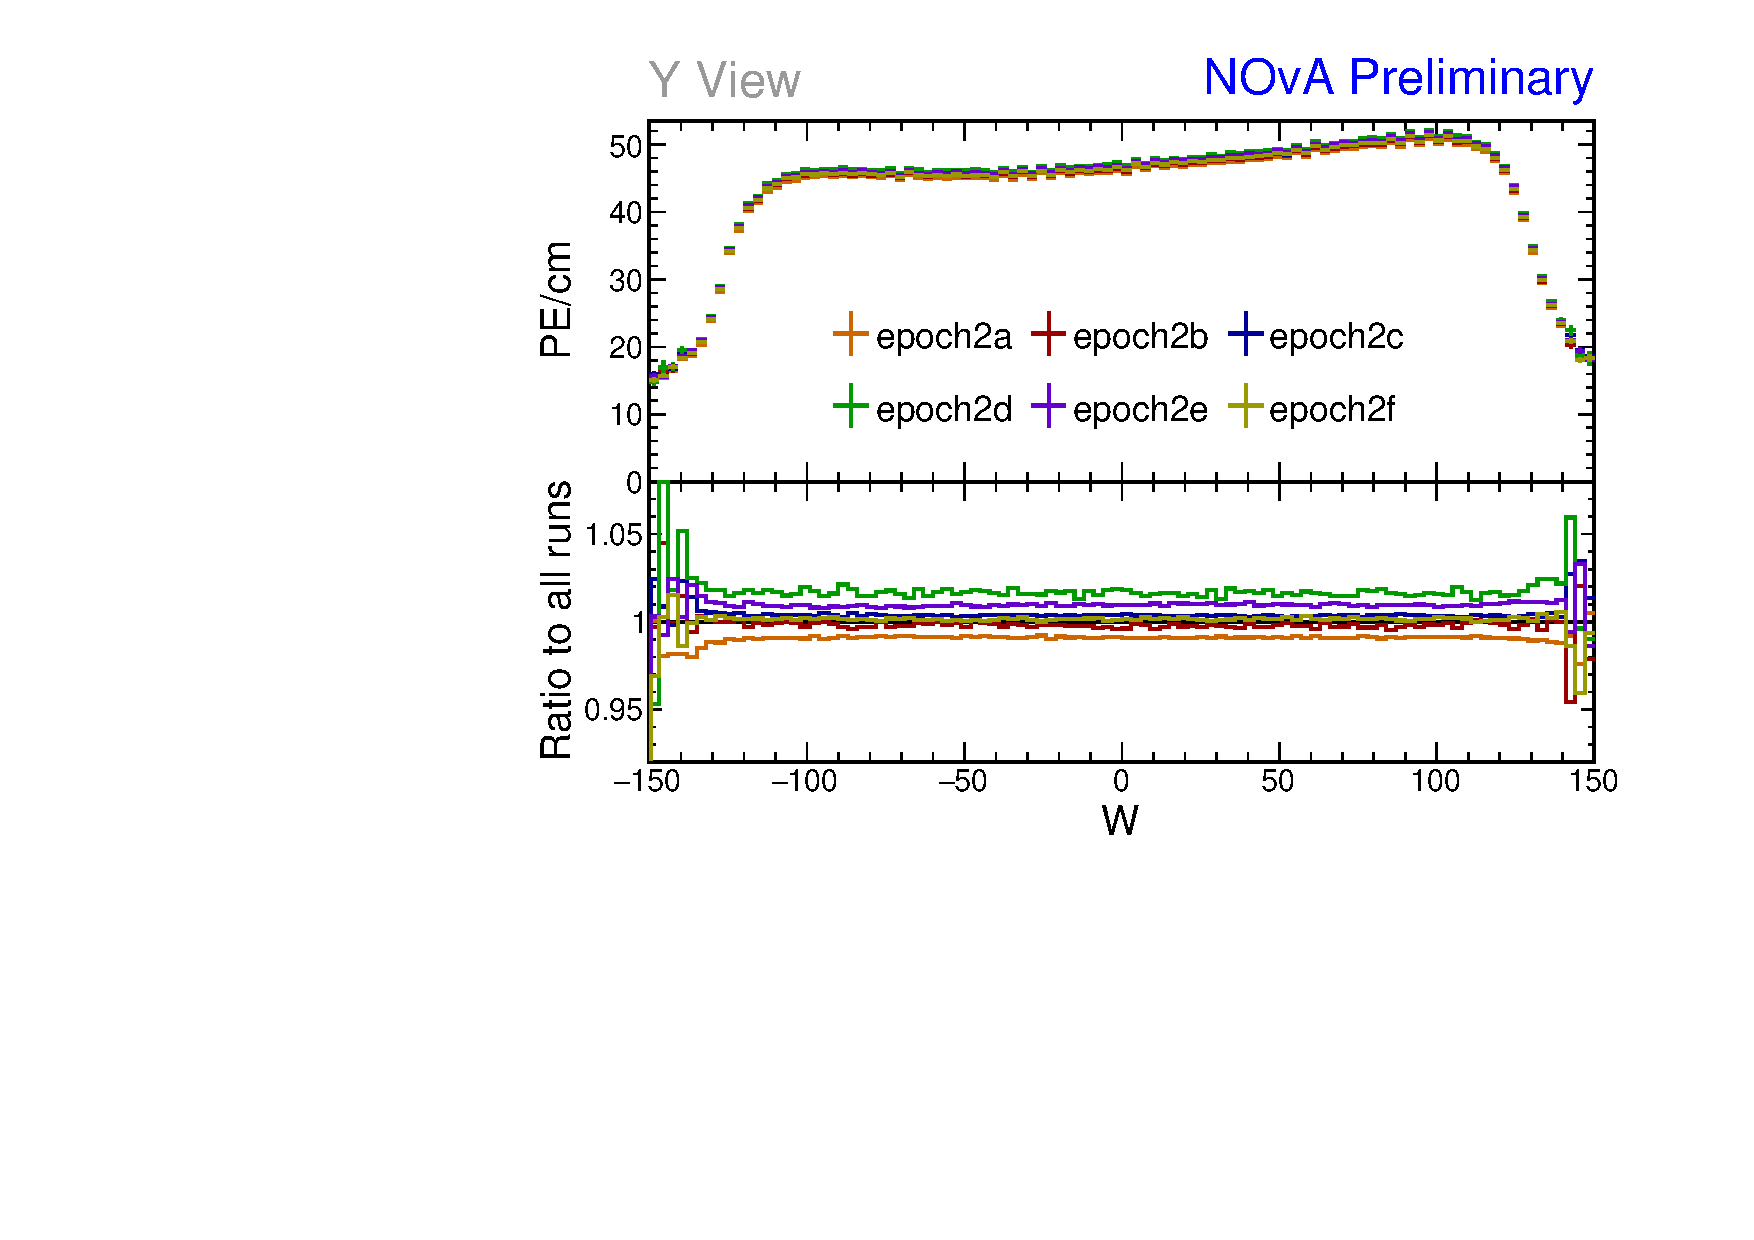
\includegraphics[width=\textwidth]{Plots/TBCalibration/Attenprofs_P2Data_WPE_corr_xy_Y_Combined.pdf}
\end{subfigure}
\begin{subfigure}[b]{0.495\textwidth}
\centering
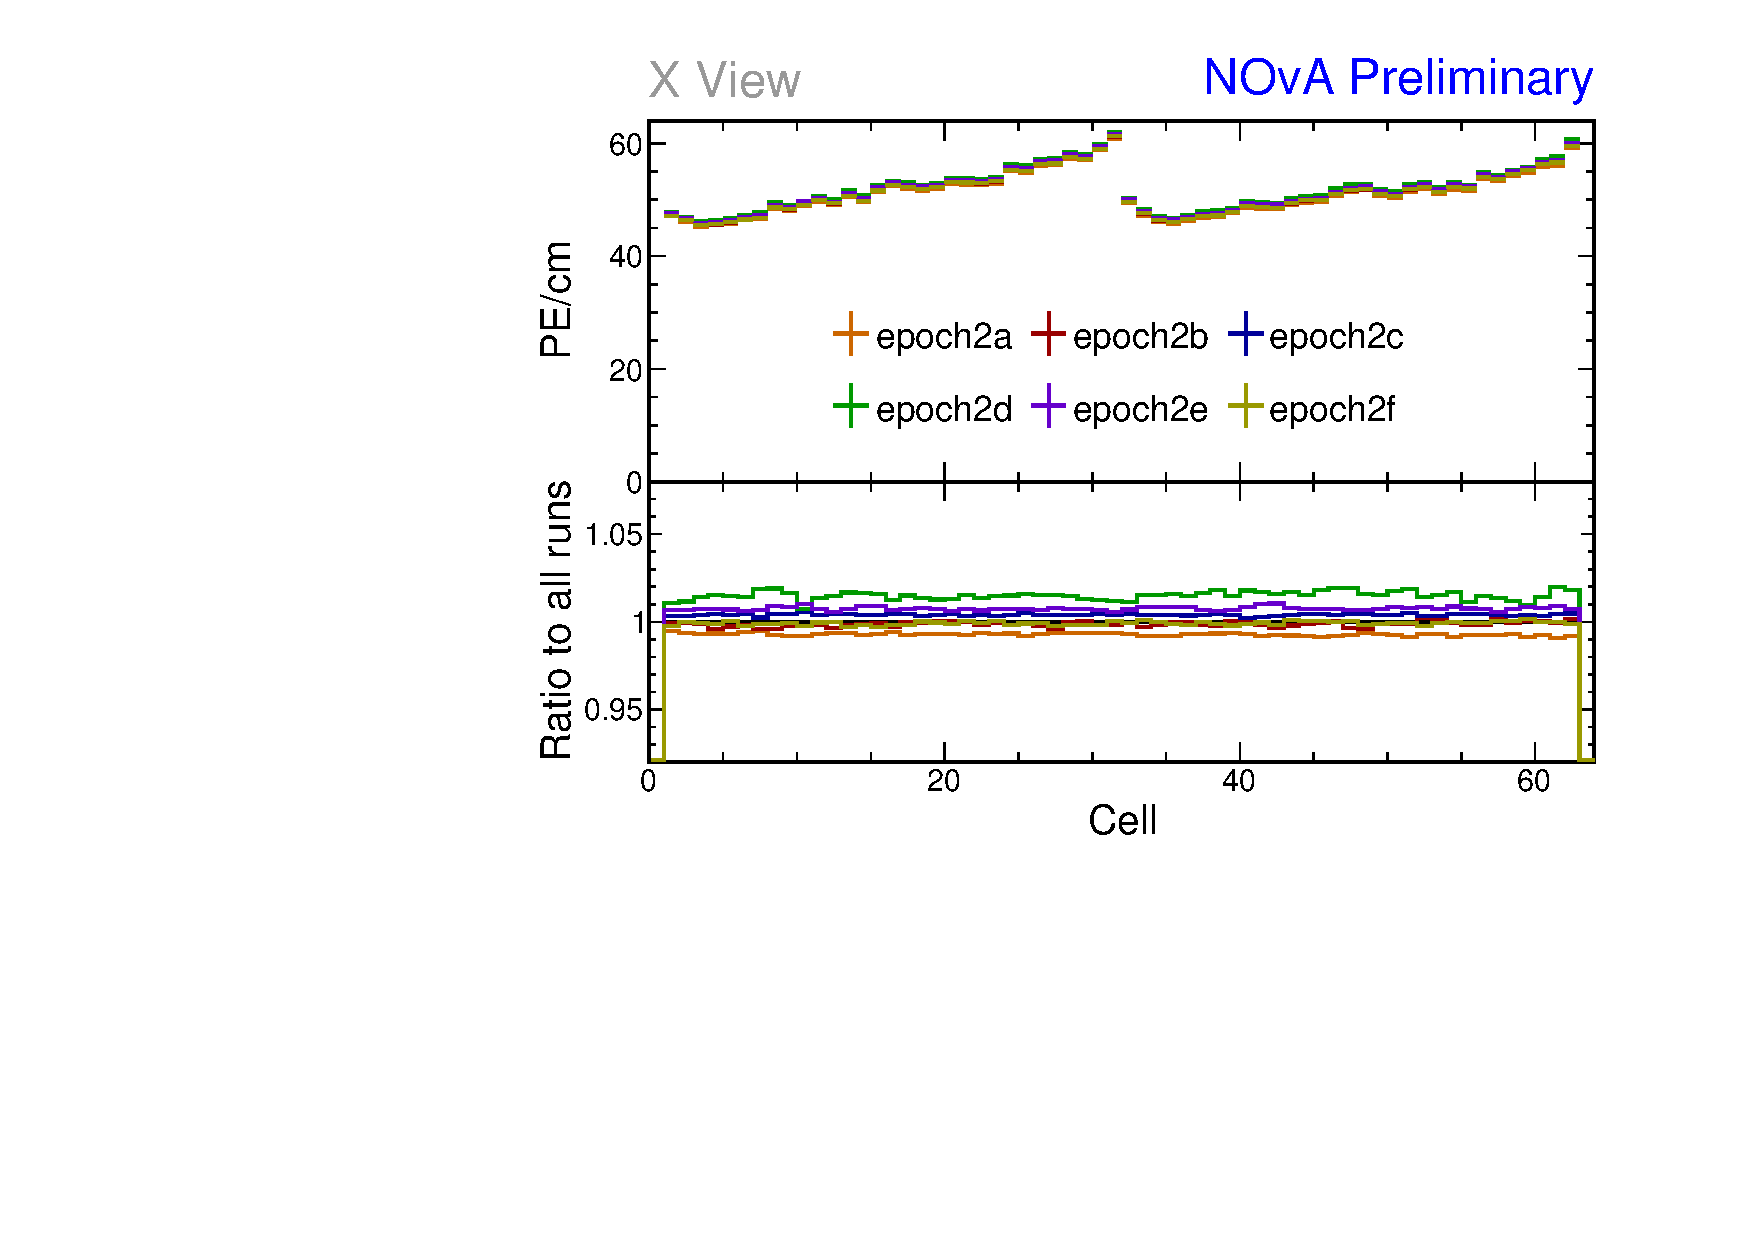
\includegraphics[width=\textwidth]{Plots/TBCalibration/Attenprofs_P2Data_CellPE_X_Combined.pdf}
\end{subfigure}
\begin{subfigure}[b]{0.495\textwidth}
\centering
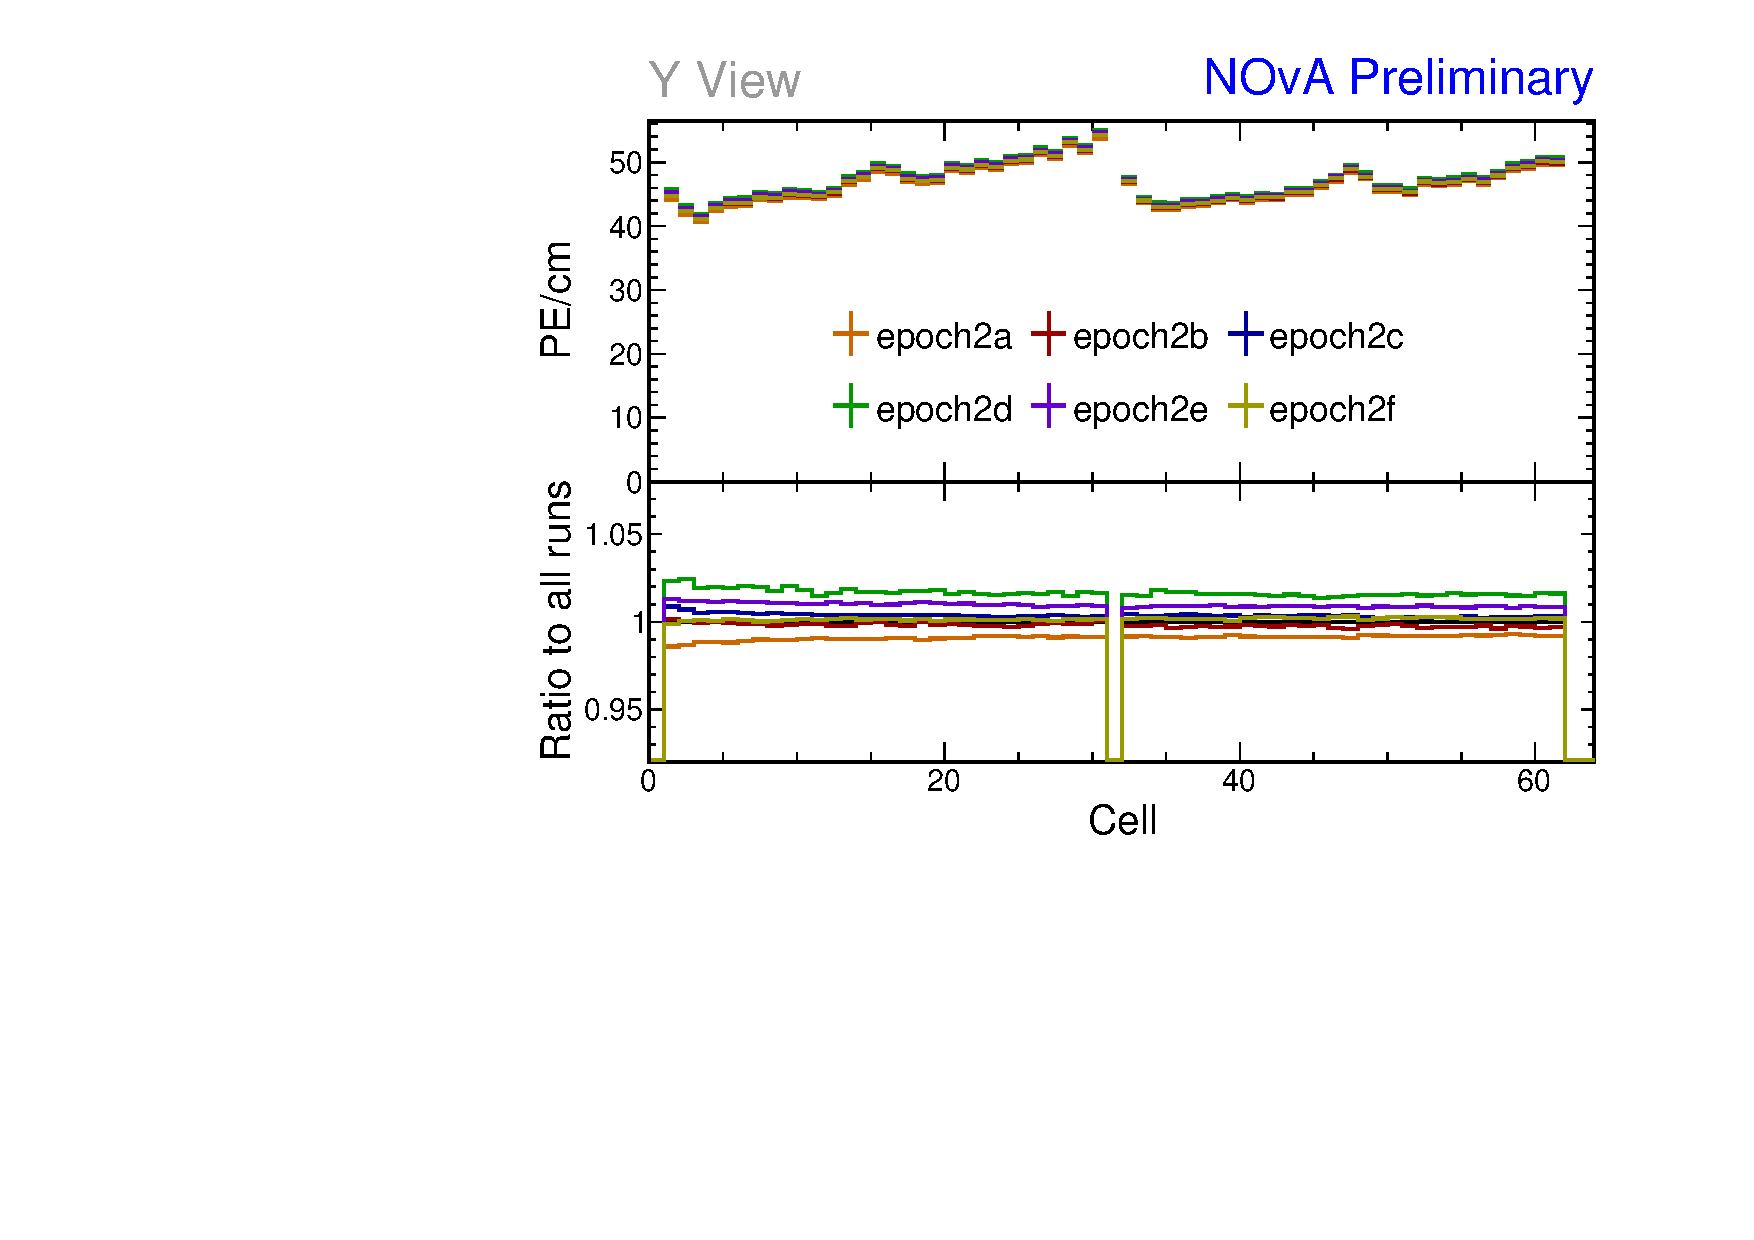
\includegraphics[width=\textwidth]{Plots/TBCalibration/Attenprofs_P2Data_CellPE_Y_Combined.pdf}
\end{subfigure}
\begin{subfigure}[b]{0.495\textwidth}
\centering
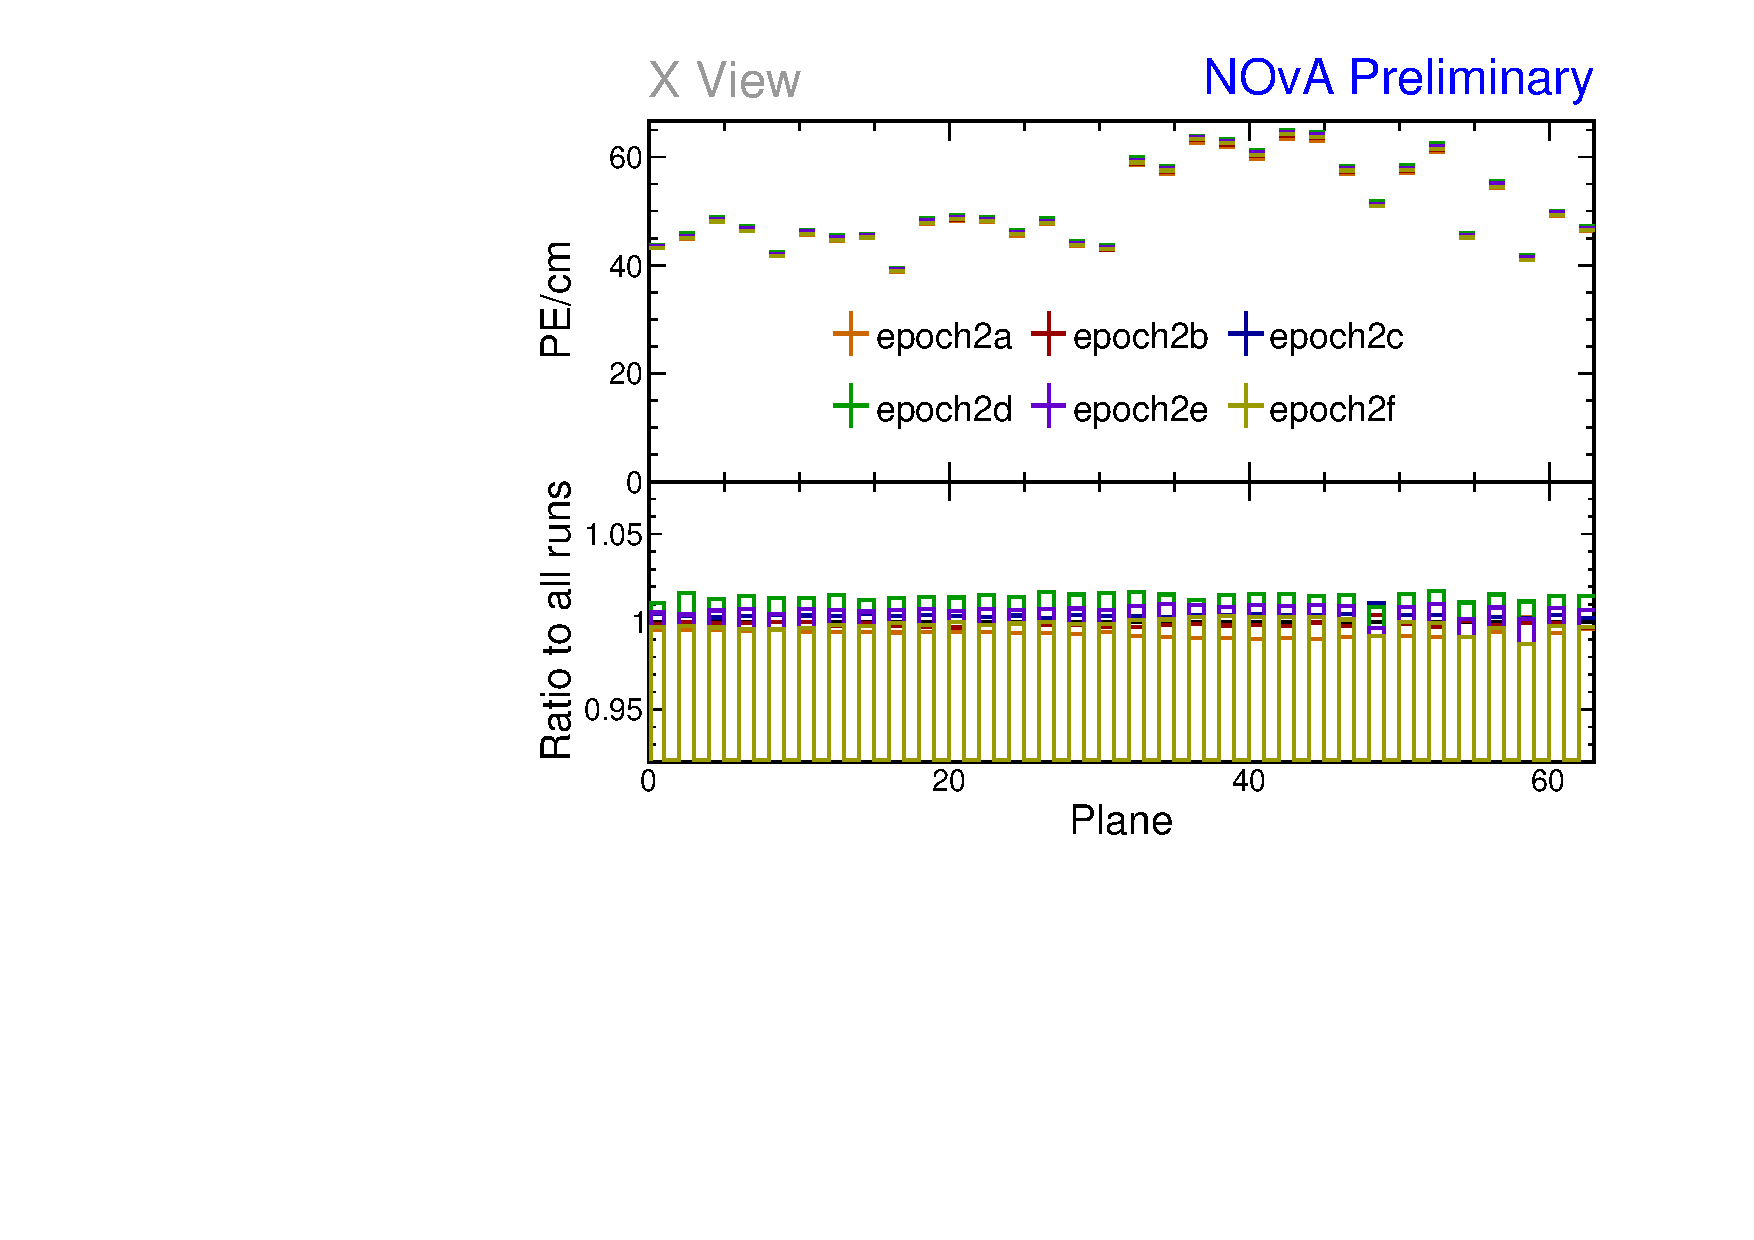
\includegraphics[width=\textwidth]{Plots/TBCalibration/Attenprofs_P2Data_PlanePE_X_Combined.pdf}
\end{subfigure}
\begin{subfigure}[b]{0.495\textwidth}
\centering
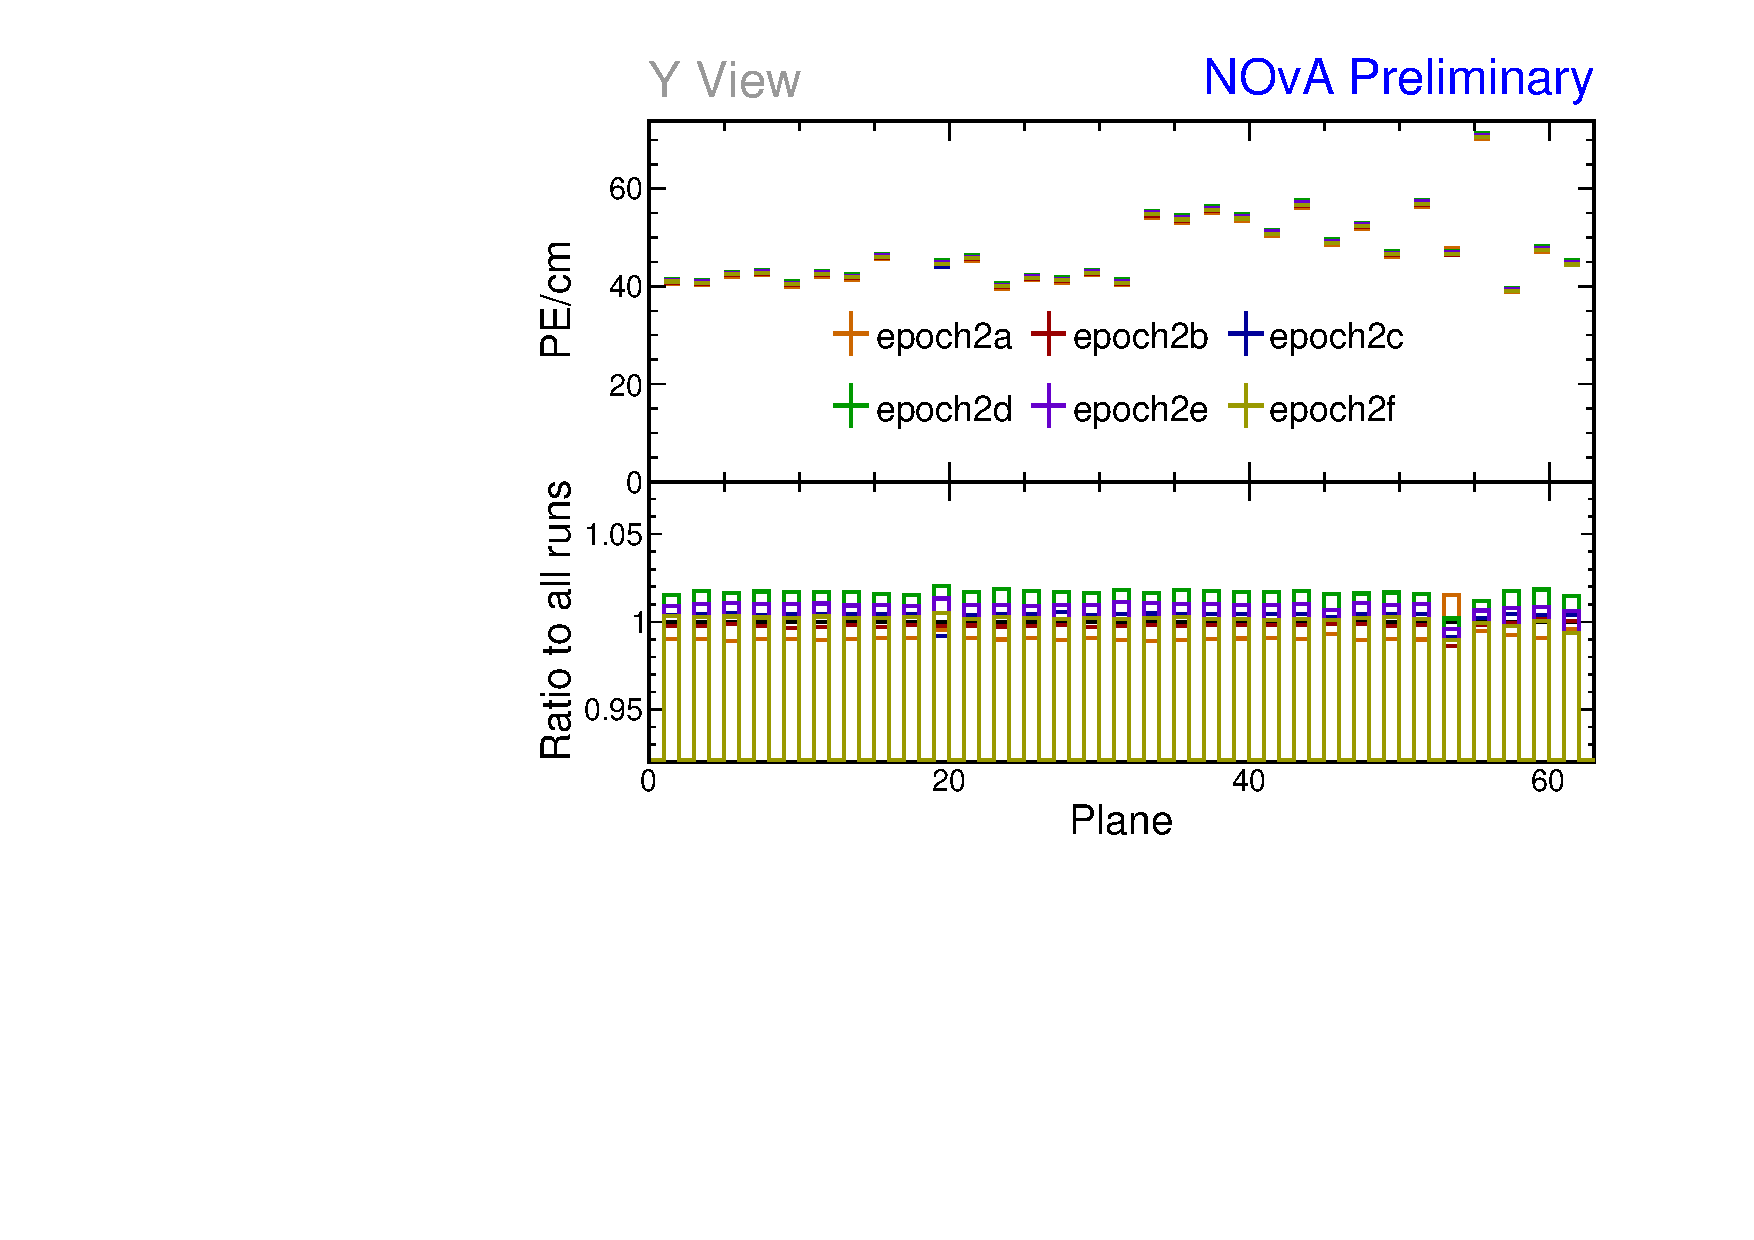
\includegraphics[width=\textwidth]{Plots/TBCalibration/Attenprofs_P2Data_PlanePE_Y_Combined.pdf}
\end{subfigure}
\caption[Uncorrected energy response along $w$, cell and plane for period 2 data]{Uncorrected average energy response as a function of the position within a cell ($w$ - top), cell number (middle), or plane number (bottom) for various epochs in the Test Beam detector period 2 data of cosmic muons hits selected for calibration. Left side shows distributions for the X view (vertical) planes and right side for the Y view (horizontal) planes. Each plot is a profile histogram, with uncertainties representing statistical variations. It is clear that there is no significant difference in shape between the various epochs. The one  exception is plane 55, which has a visibly higher energy response than the rest of the planes, especially in epoch 2a, as can be seen in the bottom right plot.}
\label{fig:Calibhist_period2}
\end{figure}

The only noticeable variation of energy response across epochs in both normalization and shape can be seen on the distributions of the energy response as a function of planes, where the uncorrected response in plane 55 is noticeably higher than the rest of the period. The exact reason for this is unknown, although it is likely caused by a fault in one of the two \glspl{FEB} that make up the plane readout.

\subsection*{Period 2 relative calibration results}

The results of the attenuation fit for period 2 are summarised in Fig.~\ref{fig:CellCentreResponsePeriod2}, showing the map of the fitted response at the centre of each cell, with blank bins representing cells that failed the calibration condition and are left uncalibrated. Summary of the relative calibration results is shown in Tab.~\ref{tab:TestBeamPeriod2RelCalibResults}. There are 199 cells that failed the calibration condition out of the total 4032 cells, constituting 4.94\% of the detector left uncalibrated for period 2. The largest contribution to the uncalibrated cells are the peripheral cells on the edge of the detector, which contain too few events due to the tricell condition.

\begin{figure}[!hbtp]
\centering
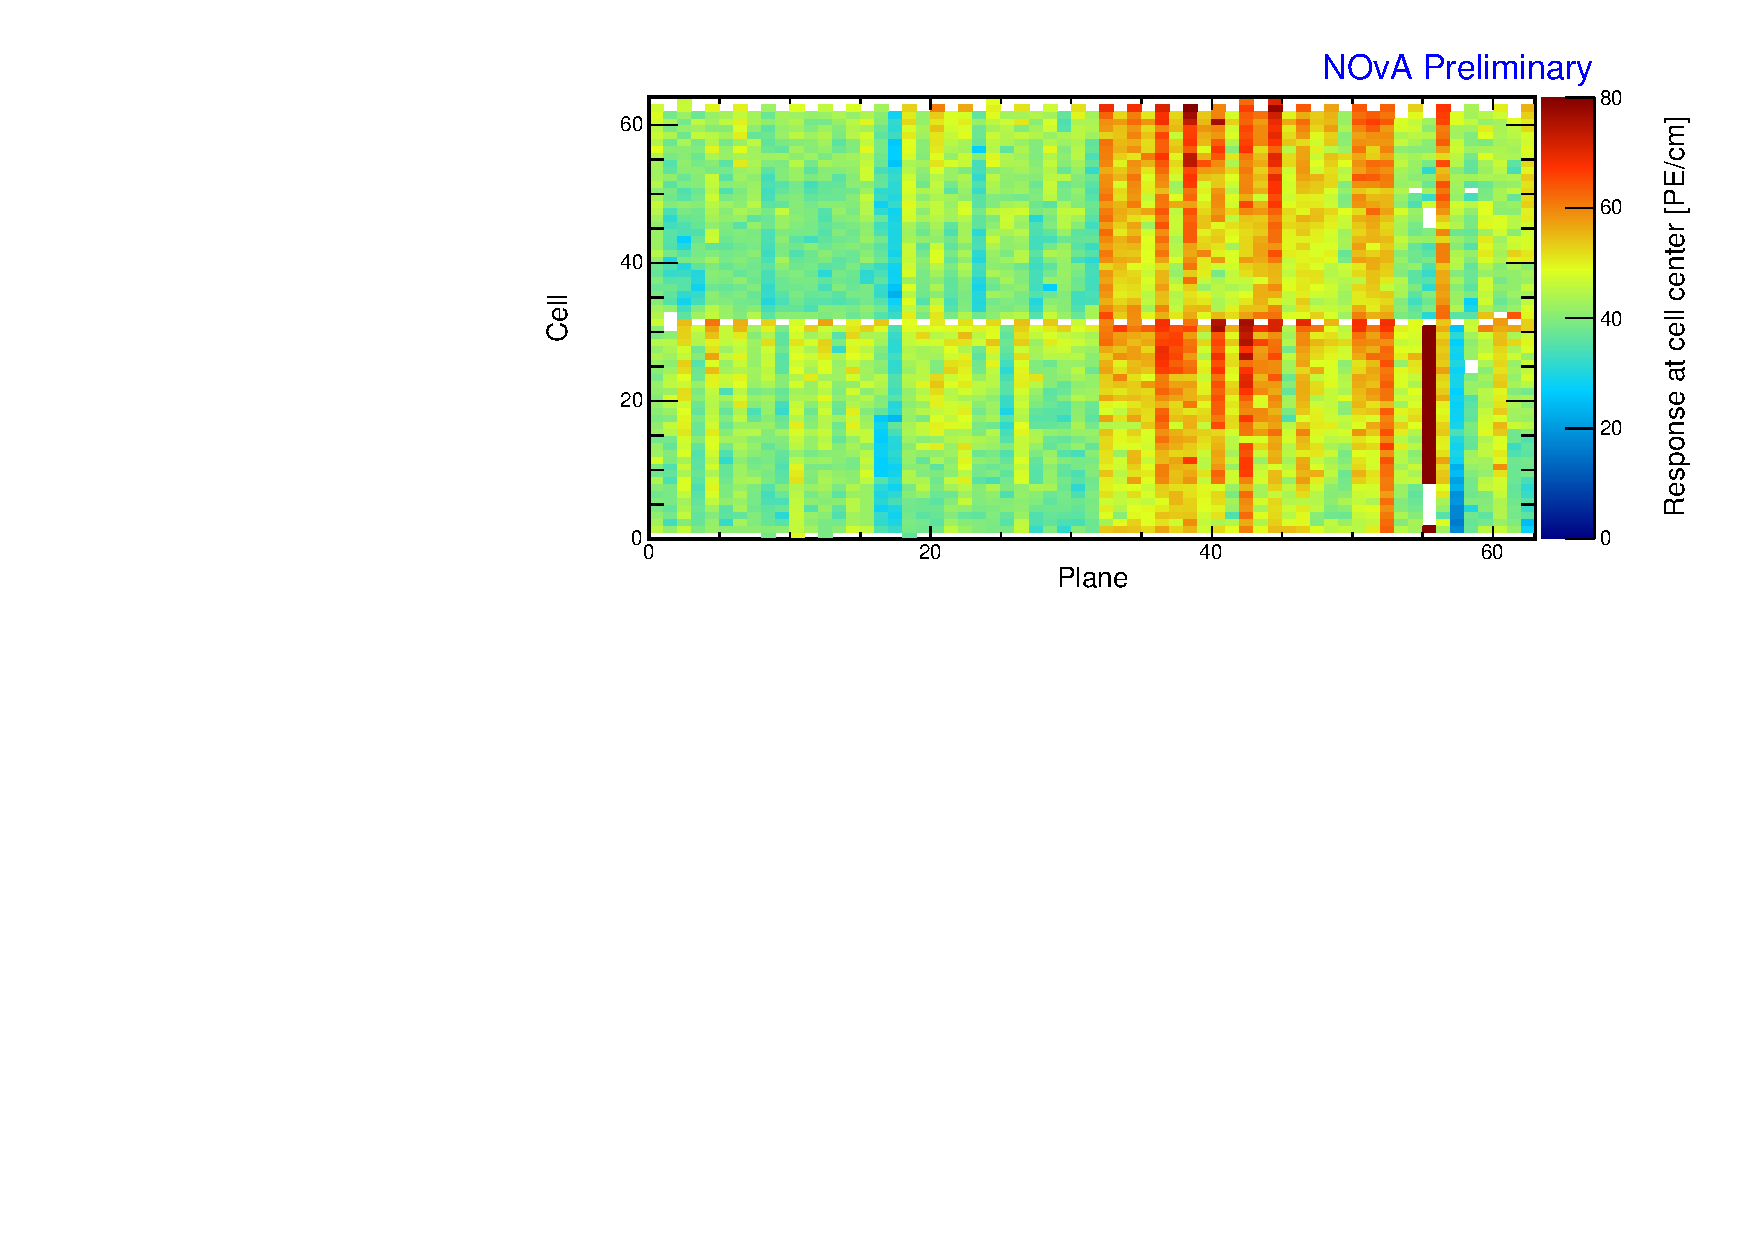
\includegraphics[width=\textwidth]{Plots/TBCalibration/CellResponseAtCentre_period2_Limited_NOvAPlotStyle.pdf}
\caption[Map of fitted response at cell centre for period 2 data]{Overview of the attenuation fit results for the Test Beam detector period 2 data. Each cell represents the result of the attenuation fit to the energy response in the centre of that cell, with blank cells failing the calibration condition $\left(\chi^2>0.2\right)$. Cells 0 and 63, which are on the edges of the detector are mostly uncalibrated due to low statistics of calibration hits. Cell 31 and 63 in horizontal planes are underfilled, showing as rows of blank cells across the detector. This affects some of their neighbouring cells, such as cells 30 and 32 in plane 1, or cells 62 in all of the horizontal planes. Cells 0-31 for planes 55 and 57 have a visibly higher (plane 55) and lower (plane 57) energy response, caused by faulty \glspl{FEB}, which for some time wrongly recorded scaled response. Cells 2-4 and 45-47 in plane 55 were dead for some time during period 2, resulting in failing the calibration condition. There are a few other uncalibrated cells, which are concentrated at the end of the detector (right hand side), which failed the calibration condition due to large fluctuations at cell edges.}
\label{fig:CellCentreResponsePeriod2}
\end{figure}

\begin{table}[!hbtp]
\centering
\caption[Summary of relative calibration results for period 2]{Summary of relative calibration results for period 2 with the uncalibrated cells divided into four categories based on the main reason of failure, all described in text.}
\def\arraystretch{1.4}
\begin{tabular}{|cl|c|c|}
\hline
\multicolumn{2}{|c|}{\textbf{Calibration status}} & \textbf{Number of cells} & \textbf{Detector proportion}\\\hline
\multicolumn{2}{|c|}{Calibrated} & $3833$ & $\unit[95.06]{\%}$\\\hline
\parbox[t]{2mm}{\multirow{4}{*}{\rotatebox[origin=c]{90}{Uncalibrated }}} & Peripheral cells & $121$ & $\unit[3.00]{\%}$\\
 & Underfilled cells & $64$ & $\unit[1.59]{\%}$\\
 & Readout & $9$ & $\unit[0.22]{\%}$\\
 & Binning & $5$ & $\unit[0.12]{\%}$\\\hline
\end{tabular}
\label{tab:TestBeamPeriod2RelCalibResults}
\end{table}

%Classic response and expected effects
Most cells have the standard response, as discussed for simulation. However, some cells have one or more regions with a drop in the energy response, as shown in Fig.~\ref{fig:AttenfitResultsPeriod2_ZippedFibers}. These low regions are a real physical effect caused by zipped, or possibly even twisted, \gls{WLS} fibres \cite{NOvA-doc-43249}. This effect is present in all the \gls{NOvA} detectors. As can be seen, the attenuation fit is capable of fitting this irregular response and therefore the relative calibration corrects for this effect in data. However, zipped fibres are not included in simulation for any of the detectors, which could potentially cause discrepancy from data due to the \gls{ADC} threshold. It was decided that this does not have a significant impact and it would not be worth the amount of work required to include all the zipped fibres into the simulation.

\begin{figure}[!hbtp]
  \begin{subfigure}{0.495\textwidth}
    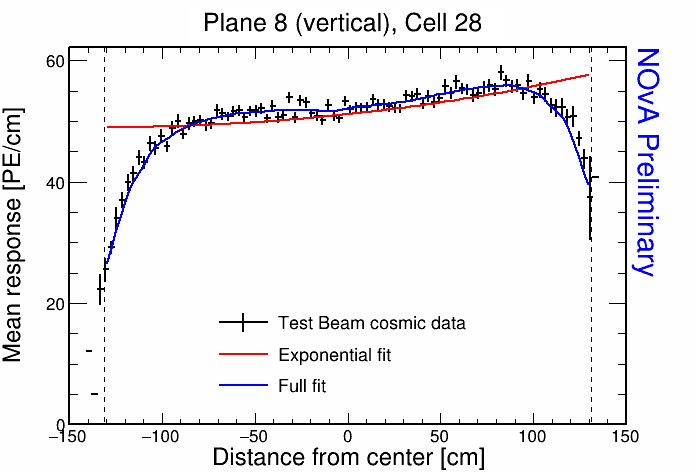
\includegraphics[width=\linewidth]{Plots/RelativeCalibrationResults/p2_008_028.png}
  \end{subfigure}
  \begin{subfigure}{0.495\textwidth}
    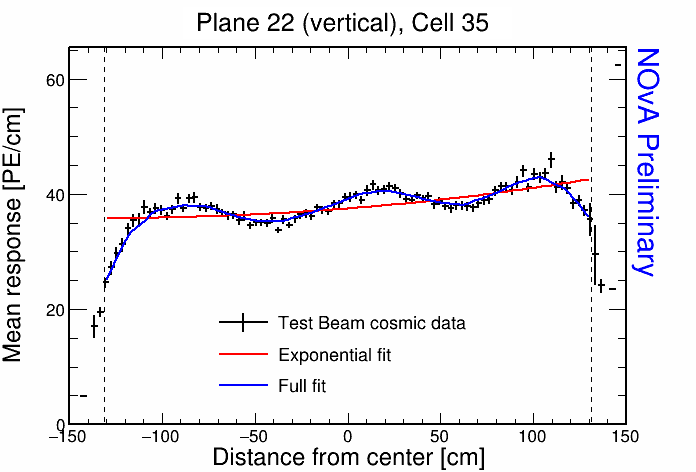
\includegraphics[width=\linewidth]{Plots/RelativeCalibrationResults/p2_022_035.png}
  \end{subfigure}
  \caption[Attenuation fits for standard cells in period 2 data]{Attenuation fits for a selection of cells in period 2. Left plot shows an example of the standard energy deposition in the Test Beam and right plot shows the effect of zipped fibres.}
  \label{fig:AttenfitResultsPeriod2_ZippedFibers}
\end{figure}

The attenuation fits for the underfilled cells fail the calibration condition as expected. On the other hand, most of their neighbouring cells in the middle of the detector (cells 30 and 32) successfully pass the calibration condition despite having fewer events. This is thanks to the decision to label the underfilled cells as bad channels, as shown in Fig.~\ref{fig:AttenfitResultsPeriod2_UnderfilledCells}. However, it appears that some cells neighbouring the underfilled cells near the edge of the detector have too few events to have satisfactory attenuation fits.

\begin{figure}[!hbtp]
  \begin{subfigure}{0.495\textwidth}
    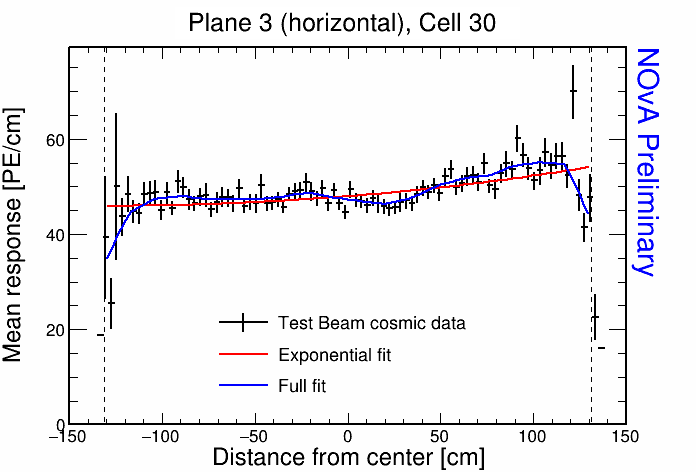
\includegraphics[width=\linewidth]{Plots/RelativeCalibrationResults/p2_003_030.png}
  \end{subfigure}
  \begin{subfigure}{0.495\textwidth}
    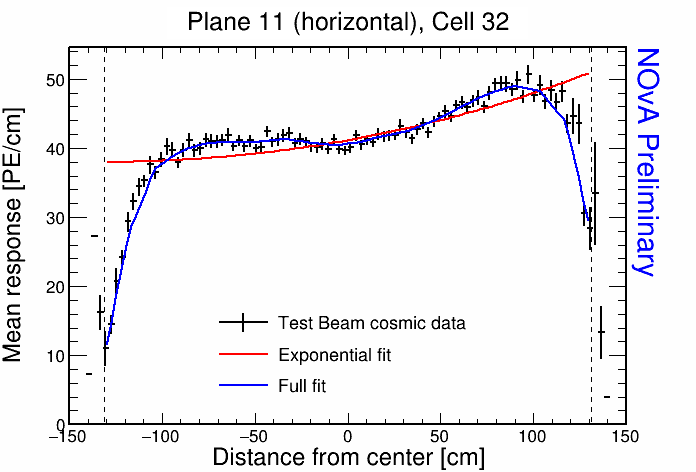
\includegraphics[width=\linewidth]{Plots/RelativeCalibrationResults/p2_011_032.png}
  \end{subfigure}
  \begin{subfigure}{0.495\textwidth}
    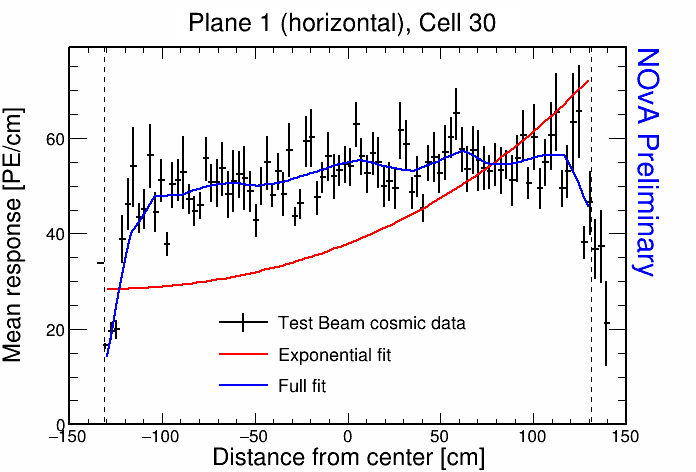
\includegraphics[width=\linewidth]{Plots/RelativeCalibrationResults/p2_001_030.png}
  \end{subfigure}
  \begin{subfigure}{0.495\textwidth}
    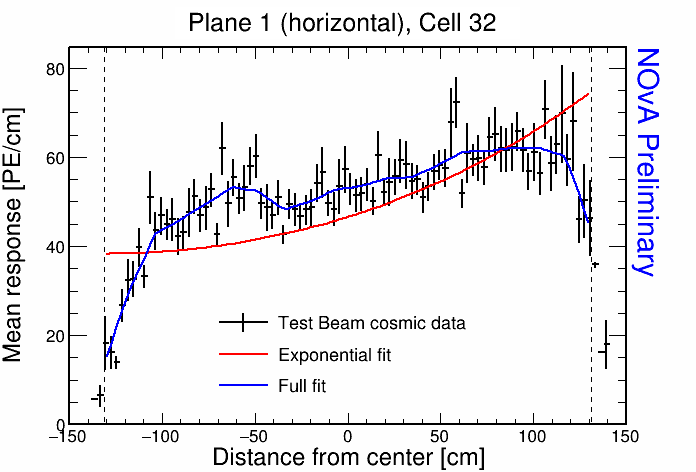
\includegraphics[width=\linewidth]{Plots/RelativeCalibrationResults/p2_001_032.png}
  \end{subfigure} 
  \caption[Attenuation fits for underfilled cells in period 2 data]{Fit to the energy response in period 2. Showing examples of cells neighbouring the underfilled cells which have fewer events and therefore larger fluctuations than the `usual' Test Beam cell. Bottom two plots show examples of neighbouring cells to the underfilled cells, specifically in plane 1, which failed the calibration condition due to low statistics. This is a result of the combined effect of being a neighbour to the underfilled cell and on the edge of the detector.}
  \label{fig:AttenfitResultsPeriod2_UnderfilledCells}
\end{figure}

%Since the underfilled cells were marked as bad channels, we didn't attempt to calibrate them. Their neighbours have fewer events due to the tricell condition, but majority of them pass the calibration condition, as shown in Fig.~\ref{fig:AttenfitResultsPerio2_UnderfilledCells}. The decision to mark the underfilled cells as bad channel was motivated by the fact that bad channels get skipped by the tricell condition and the neighbouring cells to the underfilled cells can therefore be included in calibration. The fact that majority of the neighbouring cells to the underfilled cells do get calibrated clearly proves that this was a good decision.

%The neighbouring cells in plane 1 don't pass the calibration condition due to low statistics and therefore large fluctuations, as shown in . This is likely due to a combination of the tricell condition and plane 1 being on the edge of the detector, which typically has fewer (accepted) hits than the center, as shown in Fig.~\ref{fig:Calibhist_period2}.

%Faulty readout in general
The effects  of the issues with dead channels and with faulty readout electronics occurring during period 2, which were discussed above, can be clearly seen on the map of the attenuation fit results in Fig.~\ref{fig:CellCentreResponsePeriod2} and on the attenuation fits themselves in Fig.~\ref{fig:AttenfitResultsPeriod2_ReadoutIssues}. The (temporarily) dead channel in plane 55 contains too few events to pass the calibration condition. However, the channel in plane 48 was likely dead for a shorter duration, resulting in a successful attenuation fit, despite the lower number of hits compared to a standard cell. Cells corresponding to the entire readout affected have lower number of hits, resulting in some of them having attenuation fits failing the calibration condition.  Furthermore, these cells have a strikingly different energy response, even $3\times$ larger than the average in the case of plane 55. This is due to the corresponding \glspl{APD} or \glspl{FEB} incorrectly recording a scaled-up or scaled-down energy response than the real energy deposited in the detector. The cause for this scaled recorded response is not known. Since this effect is present for all data, not only for the cosmic muons used for calibration, it is important to correctly account for it in calibration. However, there is a reason for concern, as this issue can arise even if these \glspl{FEB} (or possibly \glspl{APD}) were only affected for a limited time out of the entire calibrated period. Since we are performing the attenuation fits on the average response across the entire calibrated period, if an \gls{FEB} records a standard response for half of the time and $7\times$ larger response for the seconds half, calibration is going to assume the response was $4\times$ larger the entire time, which would be incorrect. However, since both of the affected planes are in the back of the detector, we decided to ignore this effect for period 2.

\begin{figure}[!hbtp]
  \begin{subfigure}{0.495\textwidth}
    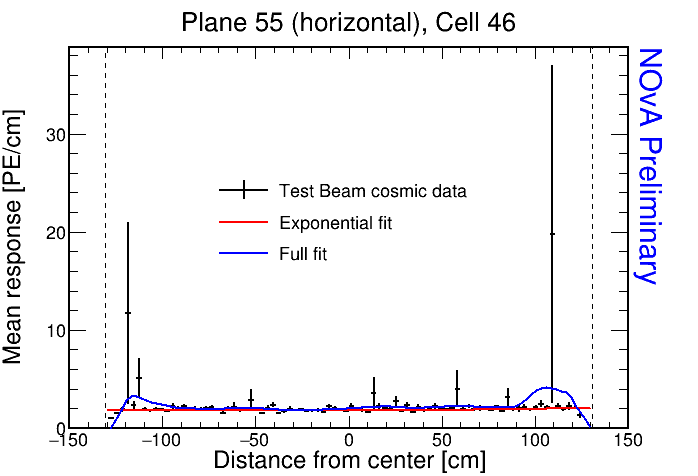
\includegraphics[width=\linewidth]{Plots/RelativeCalibrationResults/p2_055_046.png}
  \end{subfigure}
  \begin{subfigure}{0.495\textwidth}
    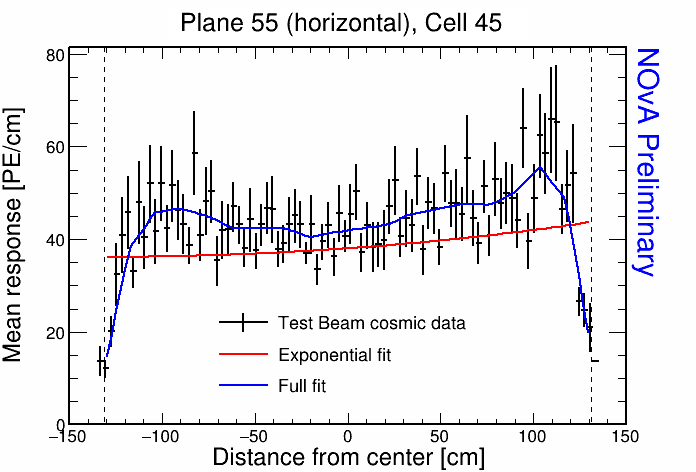
\includegraphics[width=\linewidth]{Plots/RelativeCalibrationResults/p2_055_045.png}
  \end{subfigure}
  \begin{subfigure}{0.495\textwidth}
    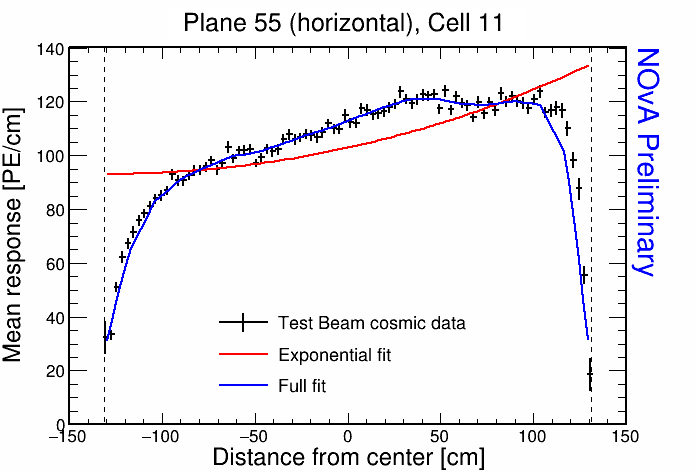
\includegraphics[width=\linewidth]{Plots/RelativeCalibrationResults/p2_055_011.png}
  \end{subfigure}
  \begin{subfigure}{0.495\textwidth}
    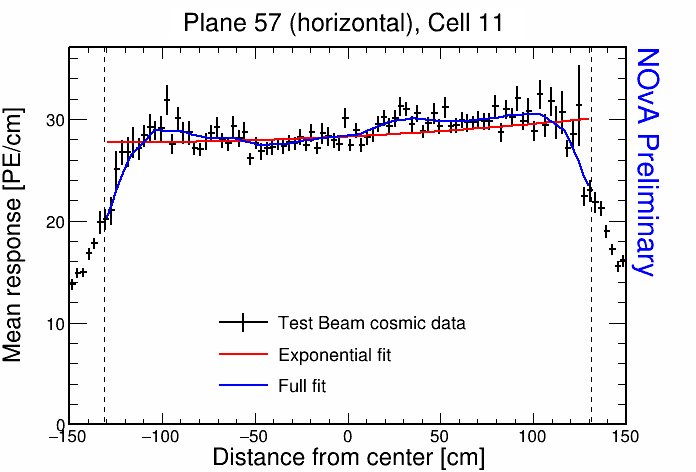
\includegraphics[width=\linewidth]{Plots/RelativeCalibrationResults/p2_057_011.png}
  \end{subfigure}
  \caption[Attenuation fits for cells with readout issues in period 2 data]{Fit to the energy response in period 2. Some channels were likely dead for some time, resulting with significantly less recorded events as shown on the top left plot. This also affect their neighbouring cells due to the tricell condition as shown on the top right. Planes 55 and 57, shown on the bottom left and bottom right plots respectively, correspond to one of the `faulty' \glspl{FEB} affected for some time. This results in a significantly different scale of energy response, which is much higher than the rest of the detector for plane 55, and smaller for plane 57.}
  \label{fig:AttenfitResultsPeriod2_ReadoutIssues}
\end{figure}

%Unexpected issue - Binning for the attenuation fits
An unexpected issue appeared for several cells located near the end of the Test Beam detector (relative to the beam). These cells have attenuation fits failing the calibration condition due to the unusually high response or a lack of events in histogram bins at the edges of the cell, as shown in Fig.~\ref{fig:AttenfitResultsPeriod2_CellEdge}. This is a combination of a real physical effect - caused by fewer hits at the edge of the detector, possibly also due to the fibre loops and fibre ends - and of the choice of binning for the attenuation profiles. All attenuation profiles for all the \gls{NOvA} detectors are created with 100 bins, extending beyond the physical dimensions of the detector. For example, in the Test Beam detector, the attenuation profiles range from $\unit[-150]{cm}$ to $\unit[150]{cm}$, while the actual half-length of a Test Beam cell is $\unit[131.07]{cm}$. This means that the attenuation profile bins near the physical edges of the cell contain fewer hits from inside of the detector, resulting in larger fluctuations. Since the attenuation fits are limited to the physical cell boundaries, these bins with larger variations can skew their results. This effect can be addressed either by changing the binning of the attenuation profiles to better match the physical dimension of the cell, by loosening the calibration condition for hits on the edges of the cell, or using larger samples for the attenuation fits to reduce variations. However, since the affected uncalibrated cells are in the end of the detector, we decided to ignore them.
%All the attenuation profiles are created with 100 bins, ranging in (-150,150) for TB, (-250,250) for ND and (-800,800) for FD. The range of the fit is the detHalfHight/Width from geometry, which is 131.07 for TB. So the bin on the edge of fit range for TB is (-132,-129).

\begin{figure}[!hbtp]
  \begin{subfigure}{0.495\textwidth}
    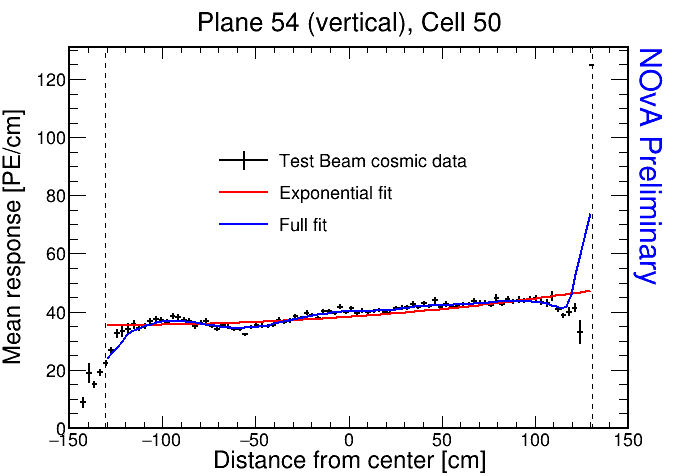
\includegraphics[width=\linewidth]{Plots/RelativeCalibrationResults/p2_054_050.png}
  \end{subfigure}
  \begin{subfigure}{0.495\textwidth}
    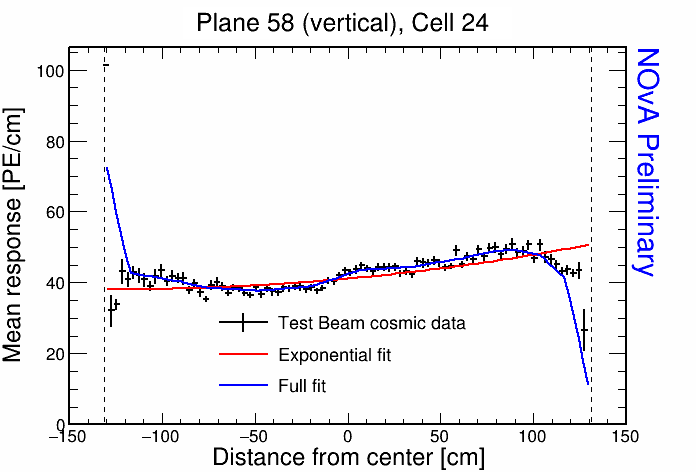
\includegraphics[width=\linewidth]{Plots/RelativeCalibrationResults/p2_058_024.png}
  \end{subfigure}
  \begin{subfigure}{0.495\textwidth}
    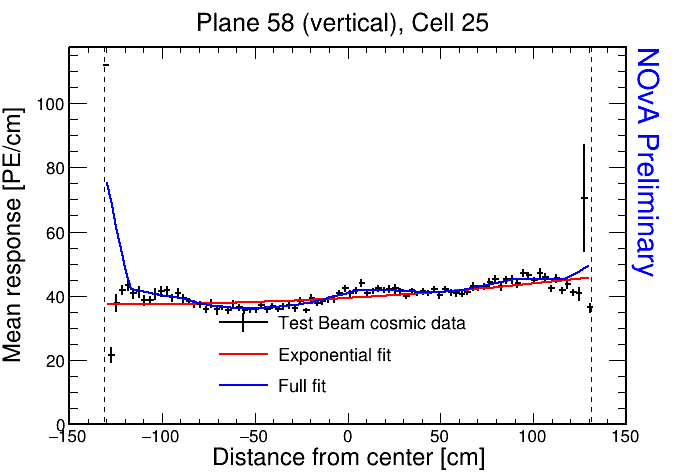
\includegraphics[width=\linewidth]{Plots/RelativeCalibrationResults/p2_058_025.png}
  \end{subfigure}
  \begin{subfigure}{0.495\textwidth}
    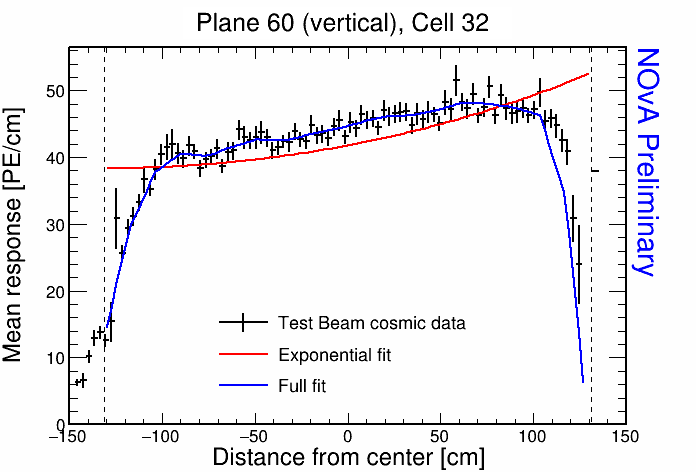
\includegraphics[width=\linewidth]{Plots/RelativeCalibrationResults/p2_060_032.png}
  \end{subfigure}
  \caption[Attenuation fits for cells with large fluctuations in period 2 data]{Fit to the energy response in period 2. Examples of cells that have an unusually high or low energy response at the edge of the cell, skewing the attenuation fits and resulting in them getting labelled as not calibrated. Cells shown on the two top plots and on the bottom left plot have a single bin on the edge of the fitted region (marked by dotted vertical lines) with noticeably higher average energy response. These anomalous bins typically only have a single entry that skews that attenuation fits and their $\chi^2$ calculations. Cell 32 in plane 60, shown in the bottom right plot, has bins on the edge of the cell with no entries, resulting in the same effect as the other cells mentioned above.}
  \label{fig:AttenfitResultsPeriod2_CellEdge}
\end{figure}

\section{Period 3 data}\label{sec:TBCalibration_period3}
The underfilled cells were refilled (or overfilled) during the period 3 data taking. This was the main motivation for dividing period 3 into individual epochs as shown in Tab.~\ref{tab:TestBeamPeriod3Epochs}. Another major event that could impact calibration is the replacement of several faulty \glspl{FEB}, which motivated the creation of epoch 3e.

\begin{table}[!hbtp]
\centering
\caption[Description of Test Beam period 3 epochs]{Test Beam period 3 epochs, their start dates and the reason for their separation.}
\def\arraystretch{1.4}
\begin{tabular}{m{0.11\textwidth} m{0.22\textwidth} m{0.55\textwidth}}
Name & Start date & Reason for creating the epoch\\\hline
Epoch 3a & January $12^{\textsf{th}}$ 2021 & Underfilled cells\\
Epoch 3b & April $21^{\textsf{st}}$ 2021 & Overfilling the back 9 horizontal planes and the 7th horizontal plane from the front\\
Epoch 3c & April $27^{\textsf{th}}$ 2021 & Overfilling of the 15 front horizontal planes (except the 7th, which was already done) and the 14th horizontal plane\\
Epoch 3d & April $30^{\textsf{th}}$ 2021 & Overfilling of the remaining 8 horizontal planes\\
Epoch 3e & May $12^{\textsf{th}}$ 2021 & FEB swaps
\end{tabular}
\label{tab:TestBeamPeriod3Epochs}
\end{table}

The refilling of the underfilled cells can be clearly seen on the cell and plane distribution of hits in Fig.~\ref{fig:CalibhistMap_period3} and on the distribution of energy deposition across horizontal (Y view) cells in Fig.~\ref{fig:Calibhist_period3}. The distributions of hits also shows a few channels that were dead for a certain time.
Additionally, the energy deposition distributions show, that one of the \glspl{FEB} was recording a scaled up/down energy  response, similarly to the faulty \glspl{FEB} in period 2. However, a can be seen in the distribution of hits, this particular faulty \gls{FEB} recorded the same number of events as were recorded in the surrounding modules. This is one of the \gls{FEB} that got replaced between epochs 3d and 3e and, as will be shown below, this is the \gls{FEB} with the largest impact on the calibration out of the faulty \glspl{FEB} replaced before the start of epoch 3e.

\begin{figure}[!hbtp]
\centering
\begin{subfigure}[b]{\textwidth}
\centering
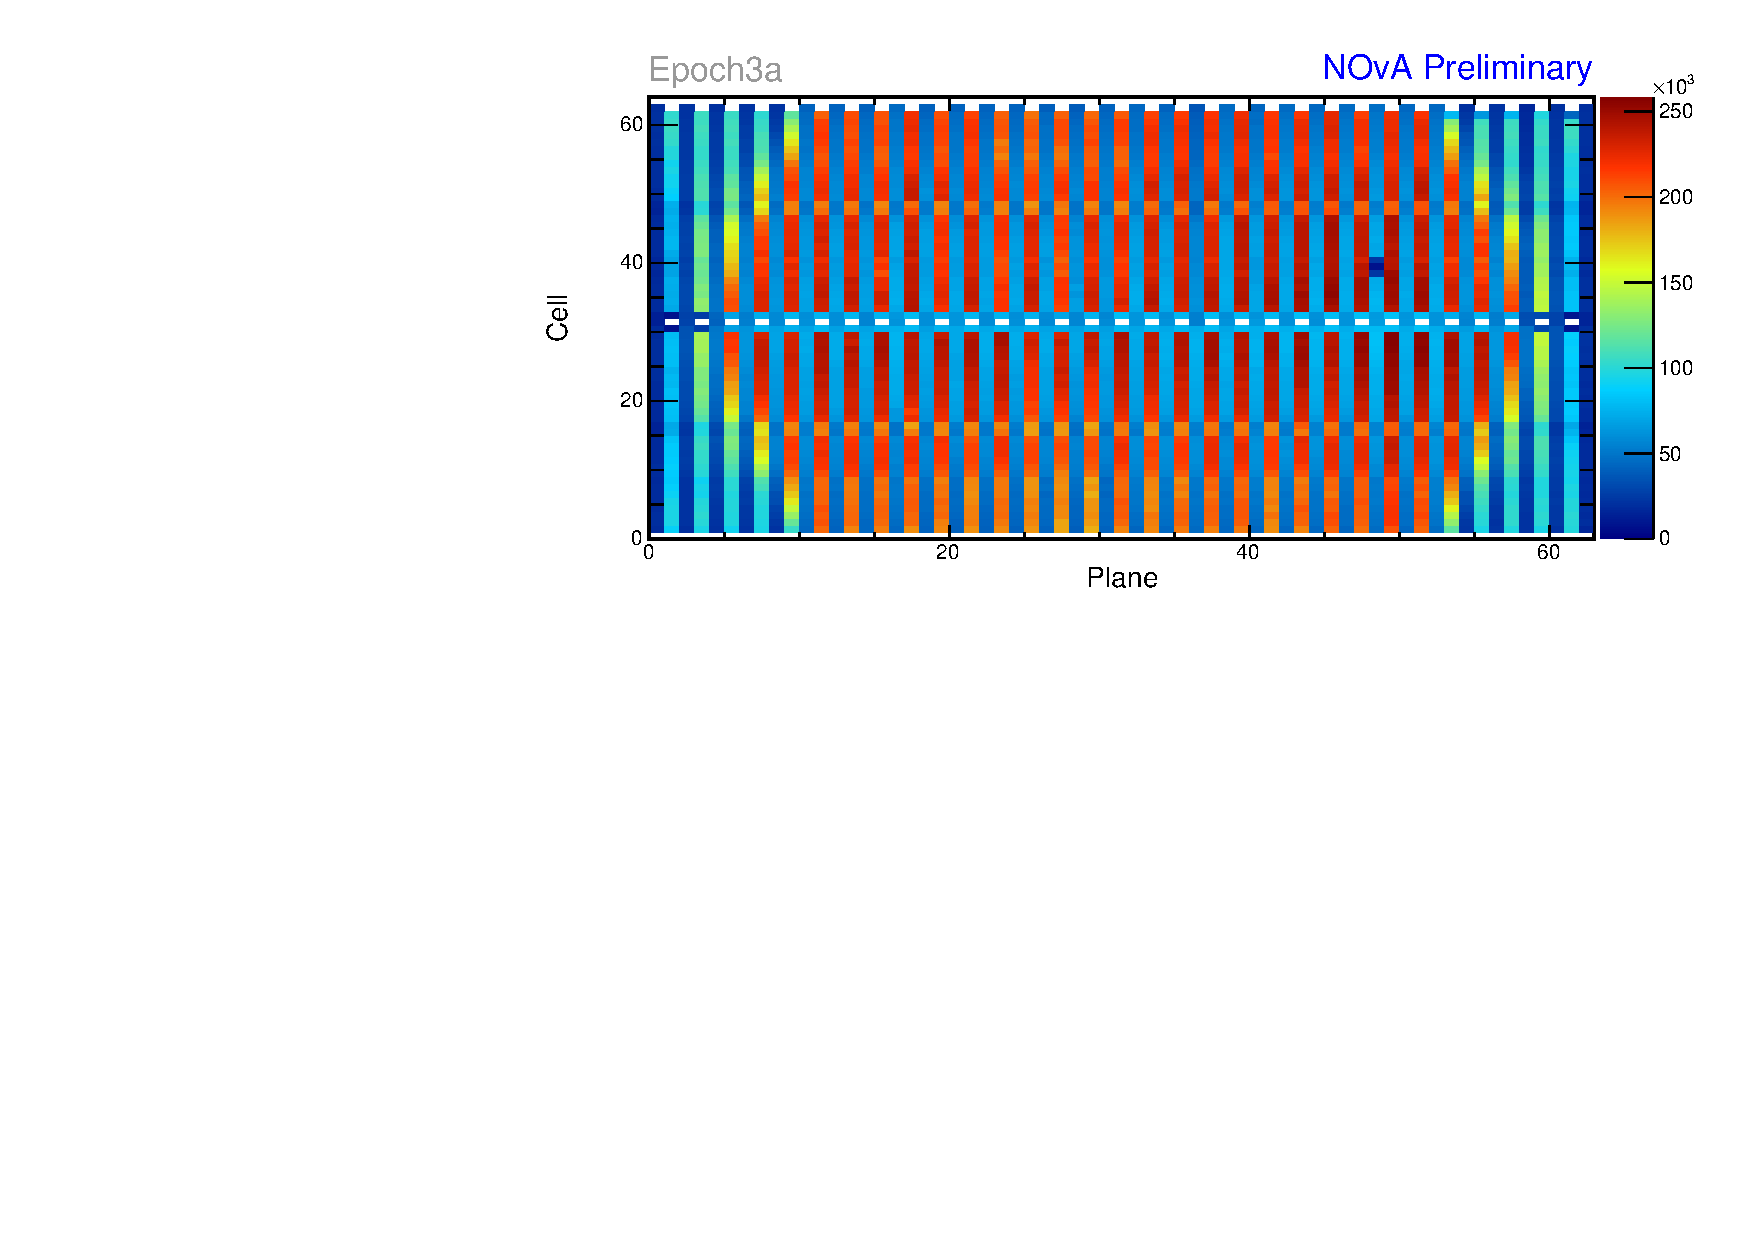
\includegraphics[width=\textwidth]{Plots/TBCalibration/Attenprofs_P3Data_CellPlane_Epoch3a.pdf}
\end{subfigure}
\begin{subfigure}[b]{\textwidth}
\centering
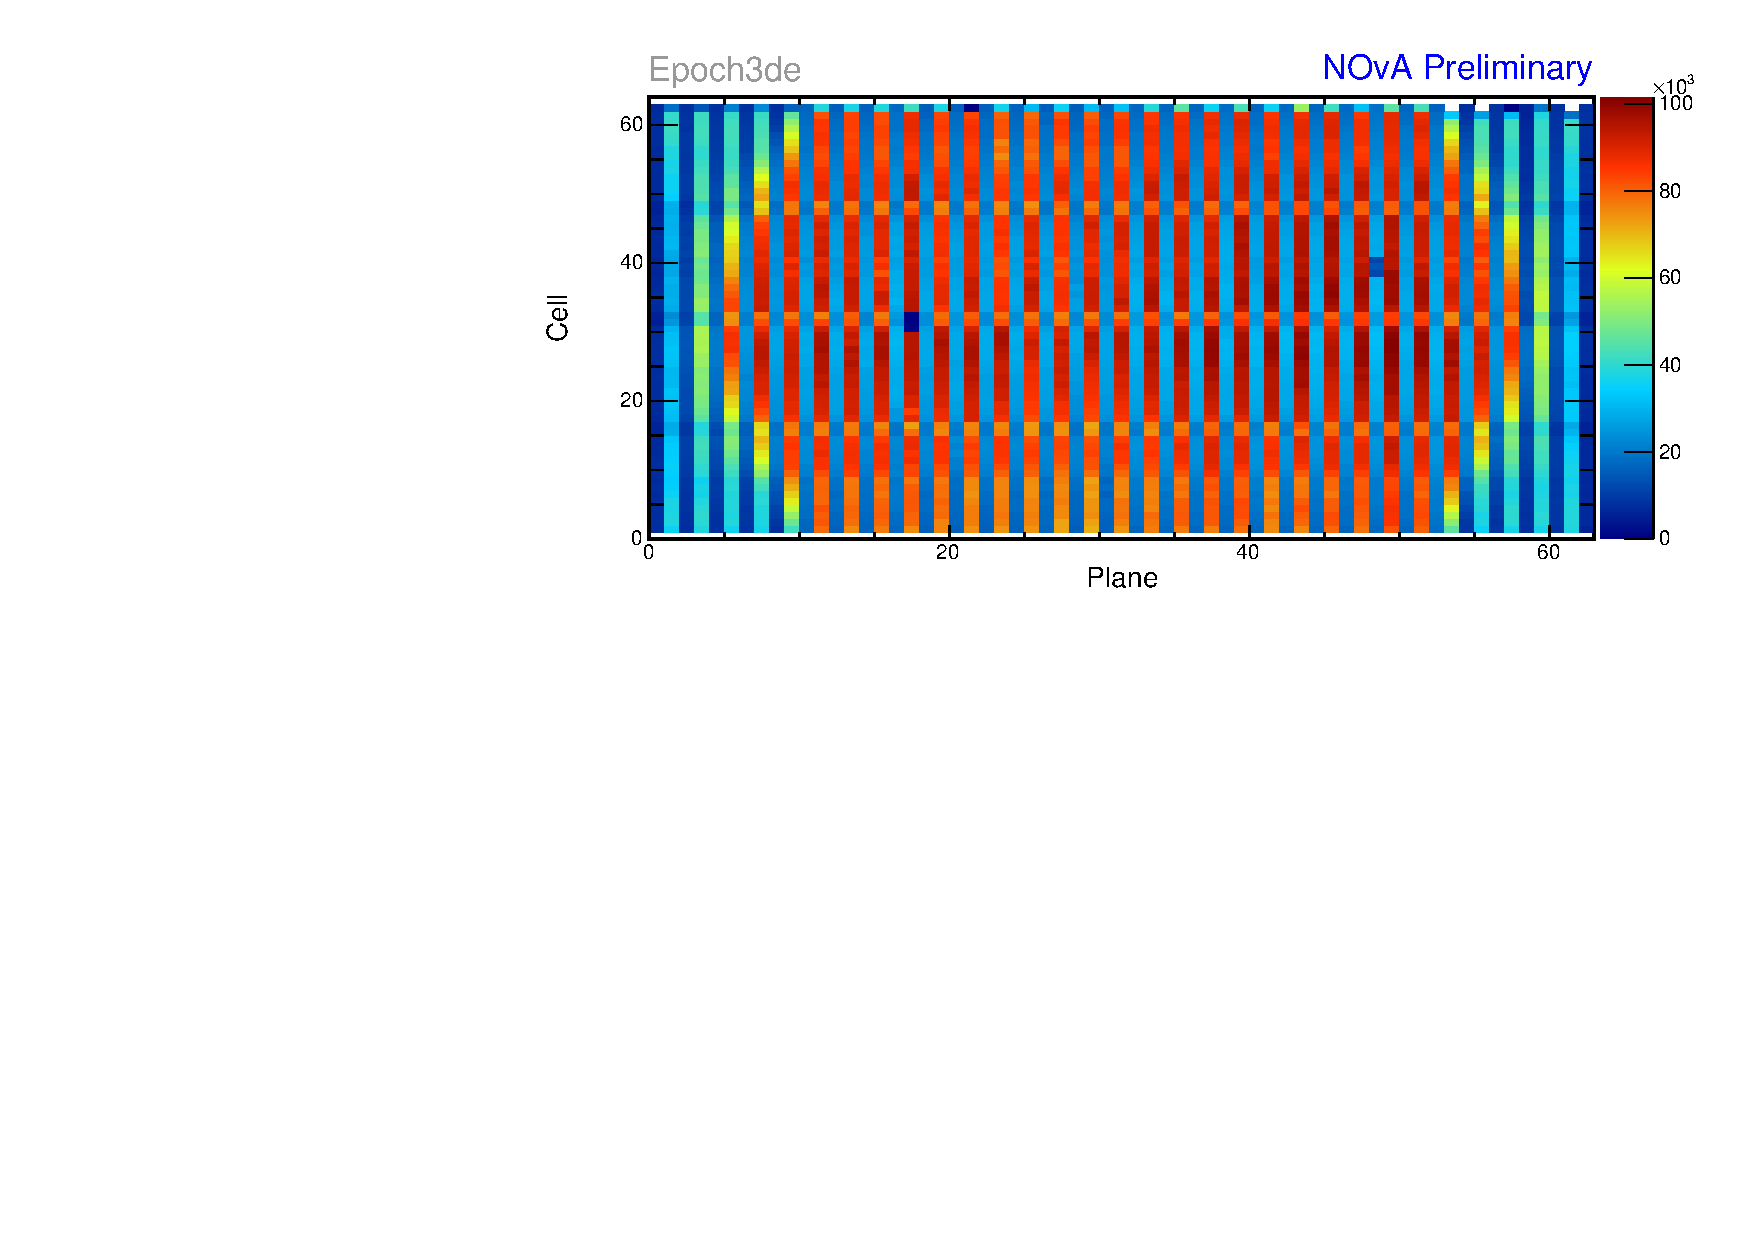
\includegraphics[width=\textwidth]{Plots/TBCalibration/Attenprofs_P3Data_CellPlane_Epoch3de.pdf}
\end{subfigure}
\caption[Plane-Cell distribution of hits for the period 3 data sample]{Distribution of events in the period 3 Test Beam data calibration sample. Comparison of the epoch 3a data before the refilling of the underfilled cells 31 and 63, clearly visible by a row of empty bins,  and the combination of epochs 3d and 3e after the full refilling. There are also several cells that experienced readout issues, specifically cell 39 in plane 48 and cell 31 in plane 18.}
\label{fig:CalibhistMap_period3}
\end{figure}

\begin{figure}[!hbtp]
\centering
\begin{subfigure}[b]{0.495\textwidth}
\centering
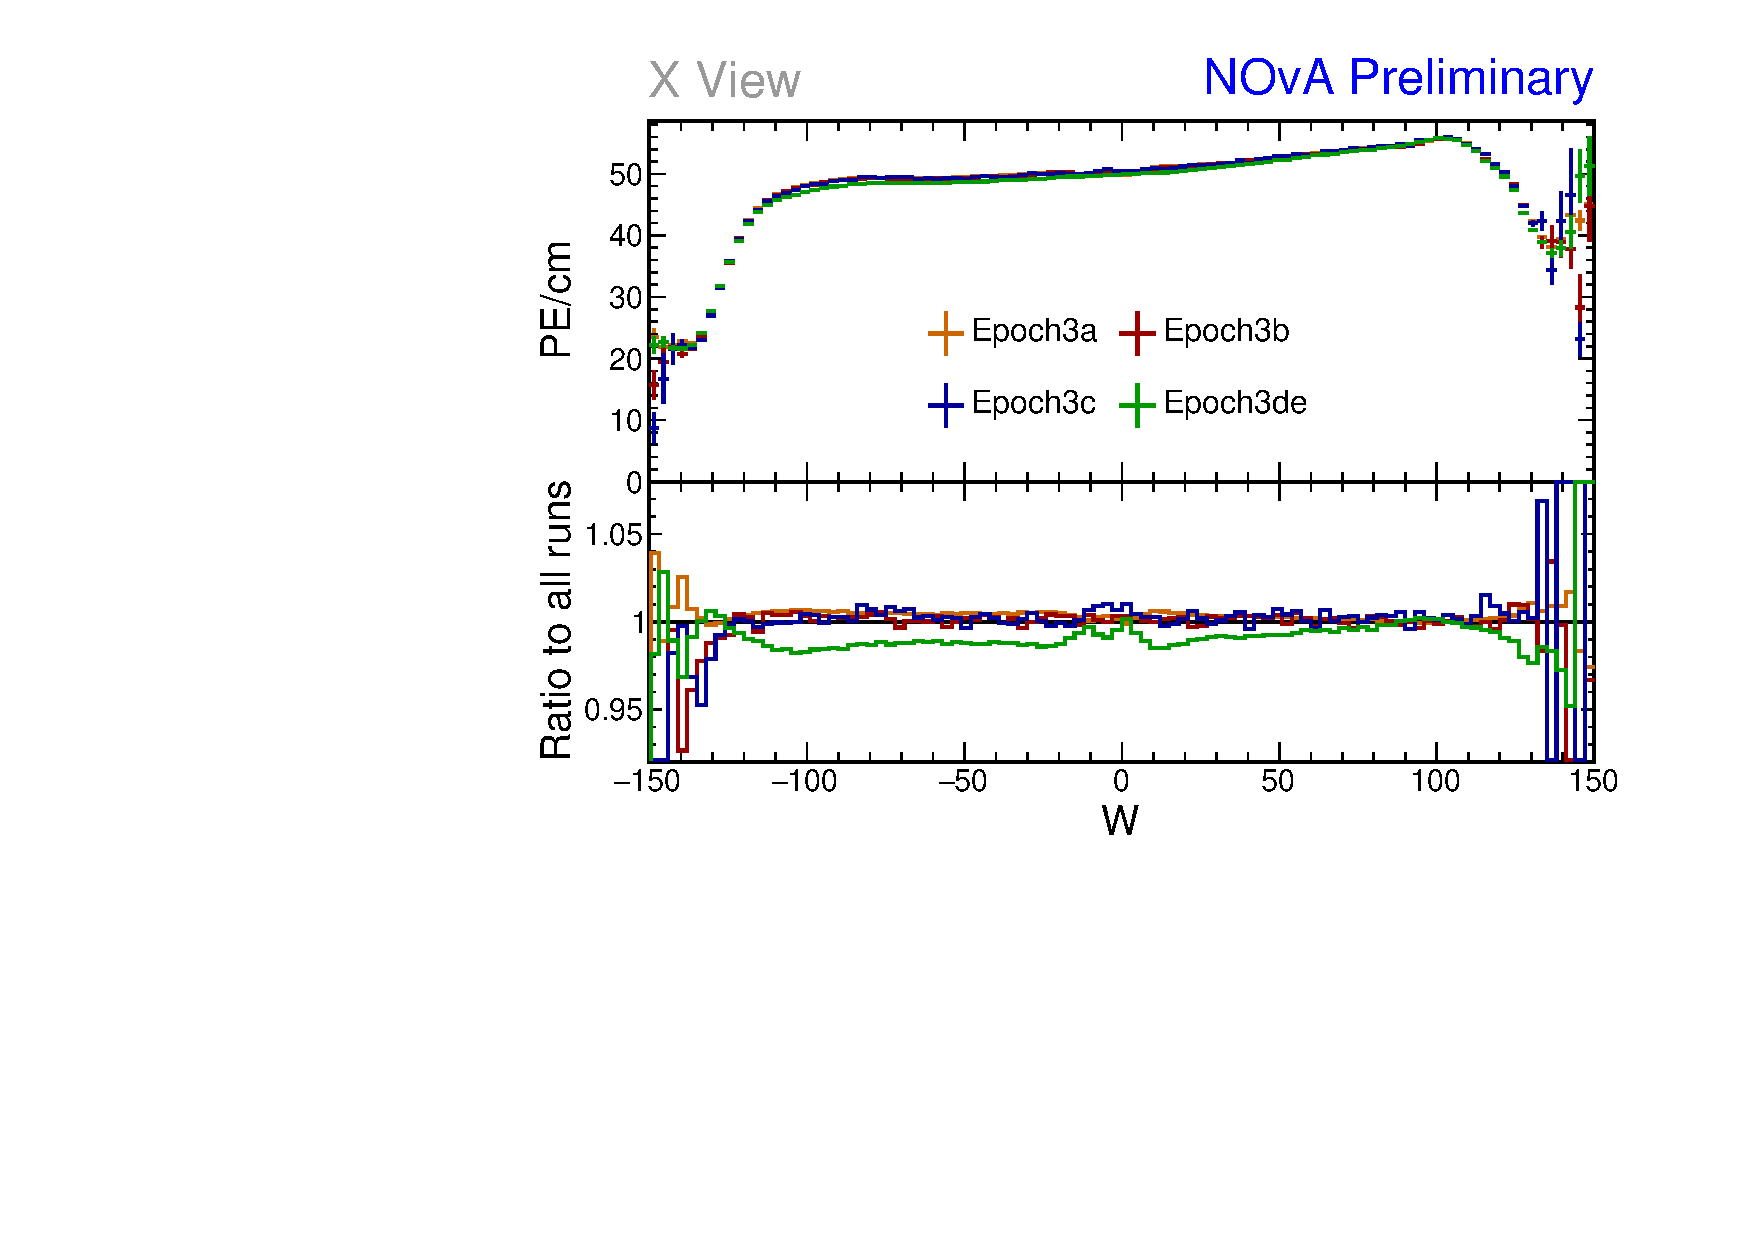
\includegraphics[width=\textwidth]{Plots/TBCalibration/Attenprofs_P3Data_WPE_corr_xy_X_Combined.pdf}
\end{subfigure}
\begin{subfigure}[b]{0.495\textwidth}
\centering
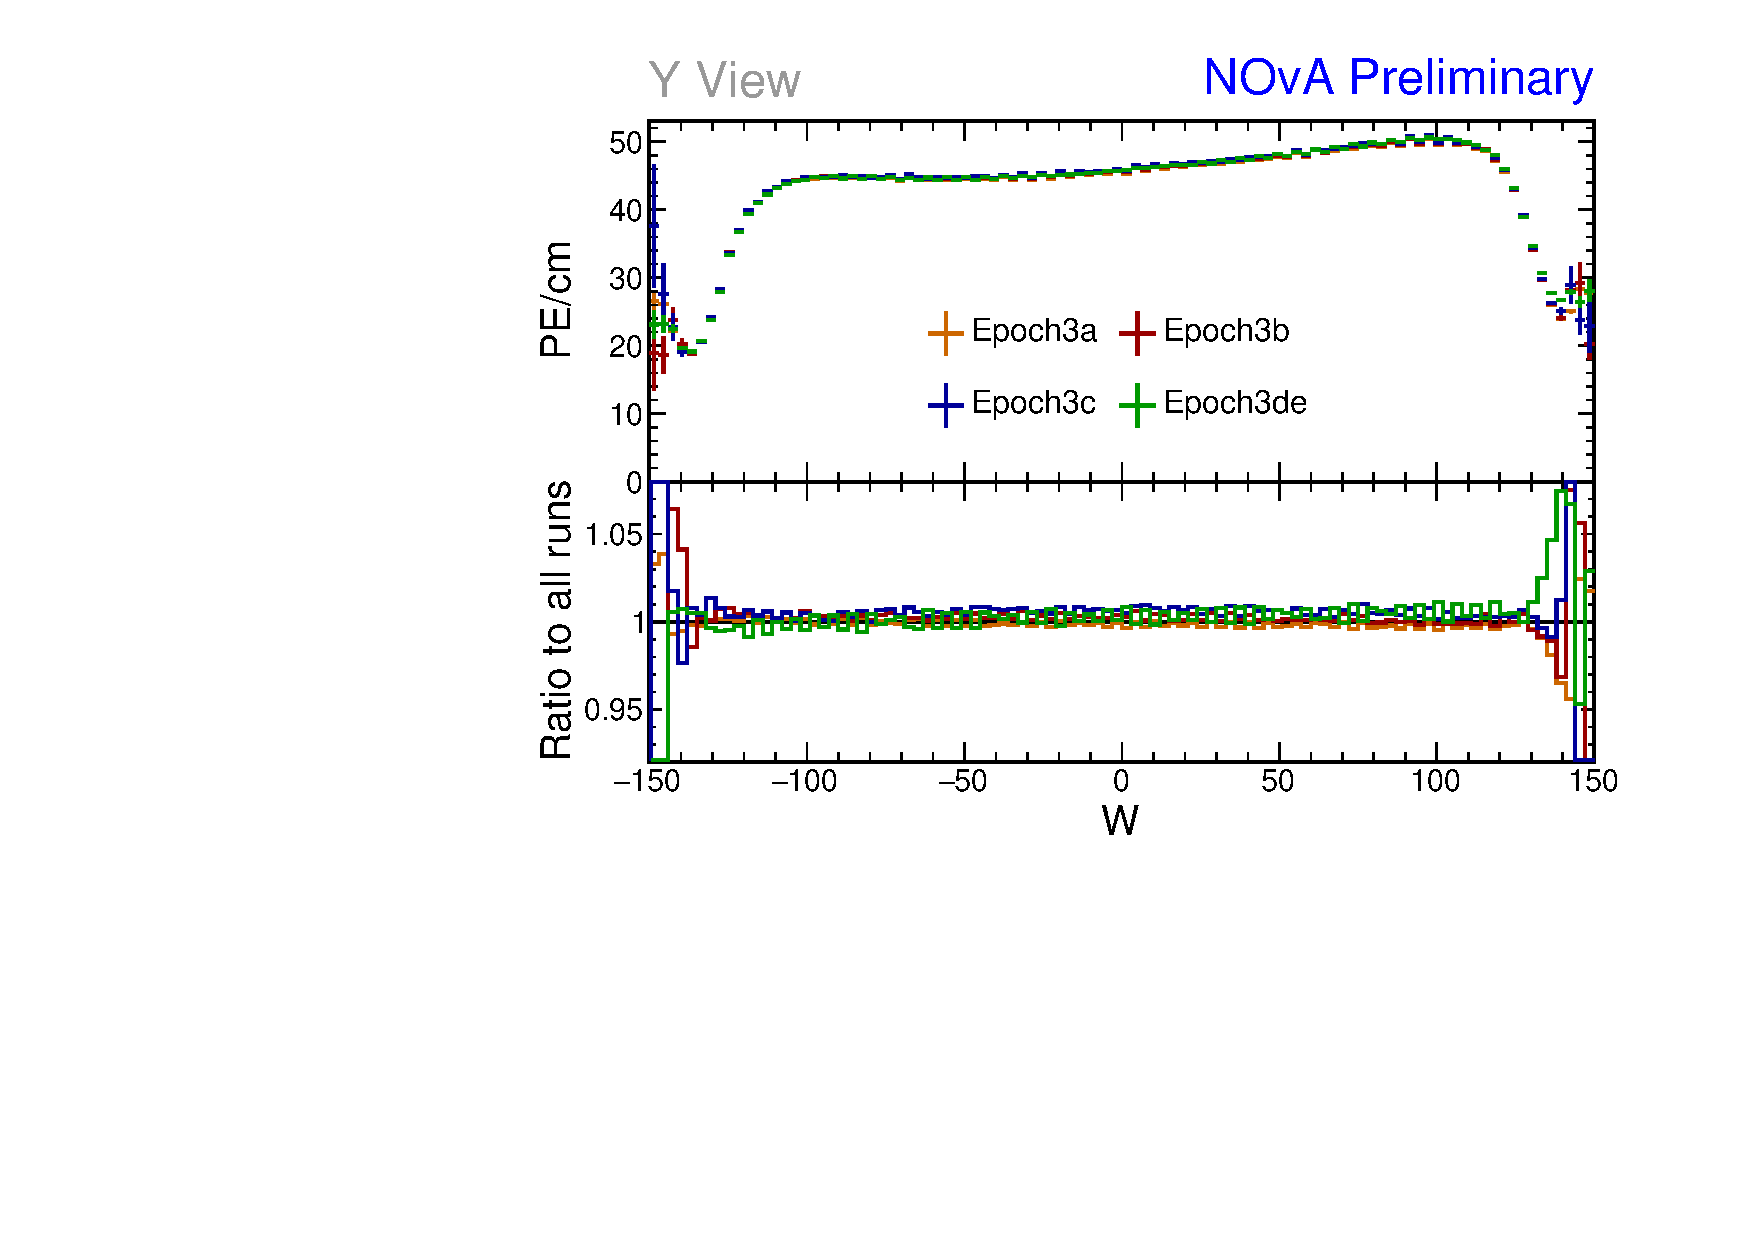
\includegraphics[width=\textwidth]{Plots/TBCalibration/Attenprofs_P3Data_WPE_corr_xy_Y_Combined.pdf}
\end{subfigure}
\begin{subfigure}[b]{0.495\textwidth}
\centering
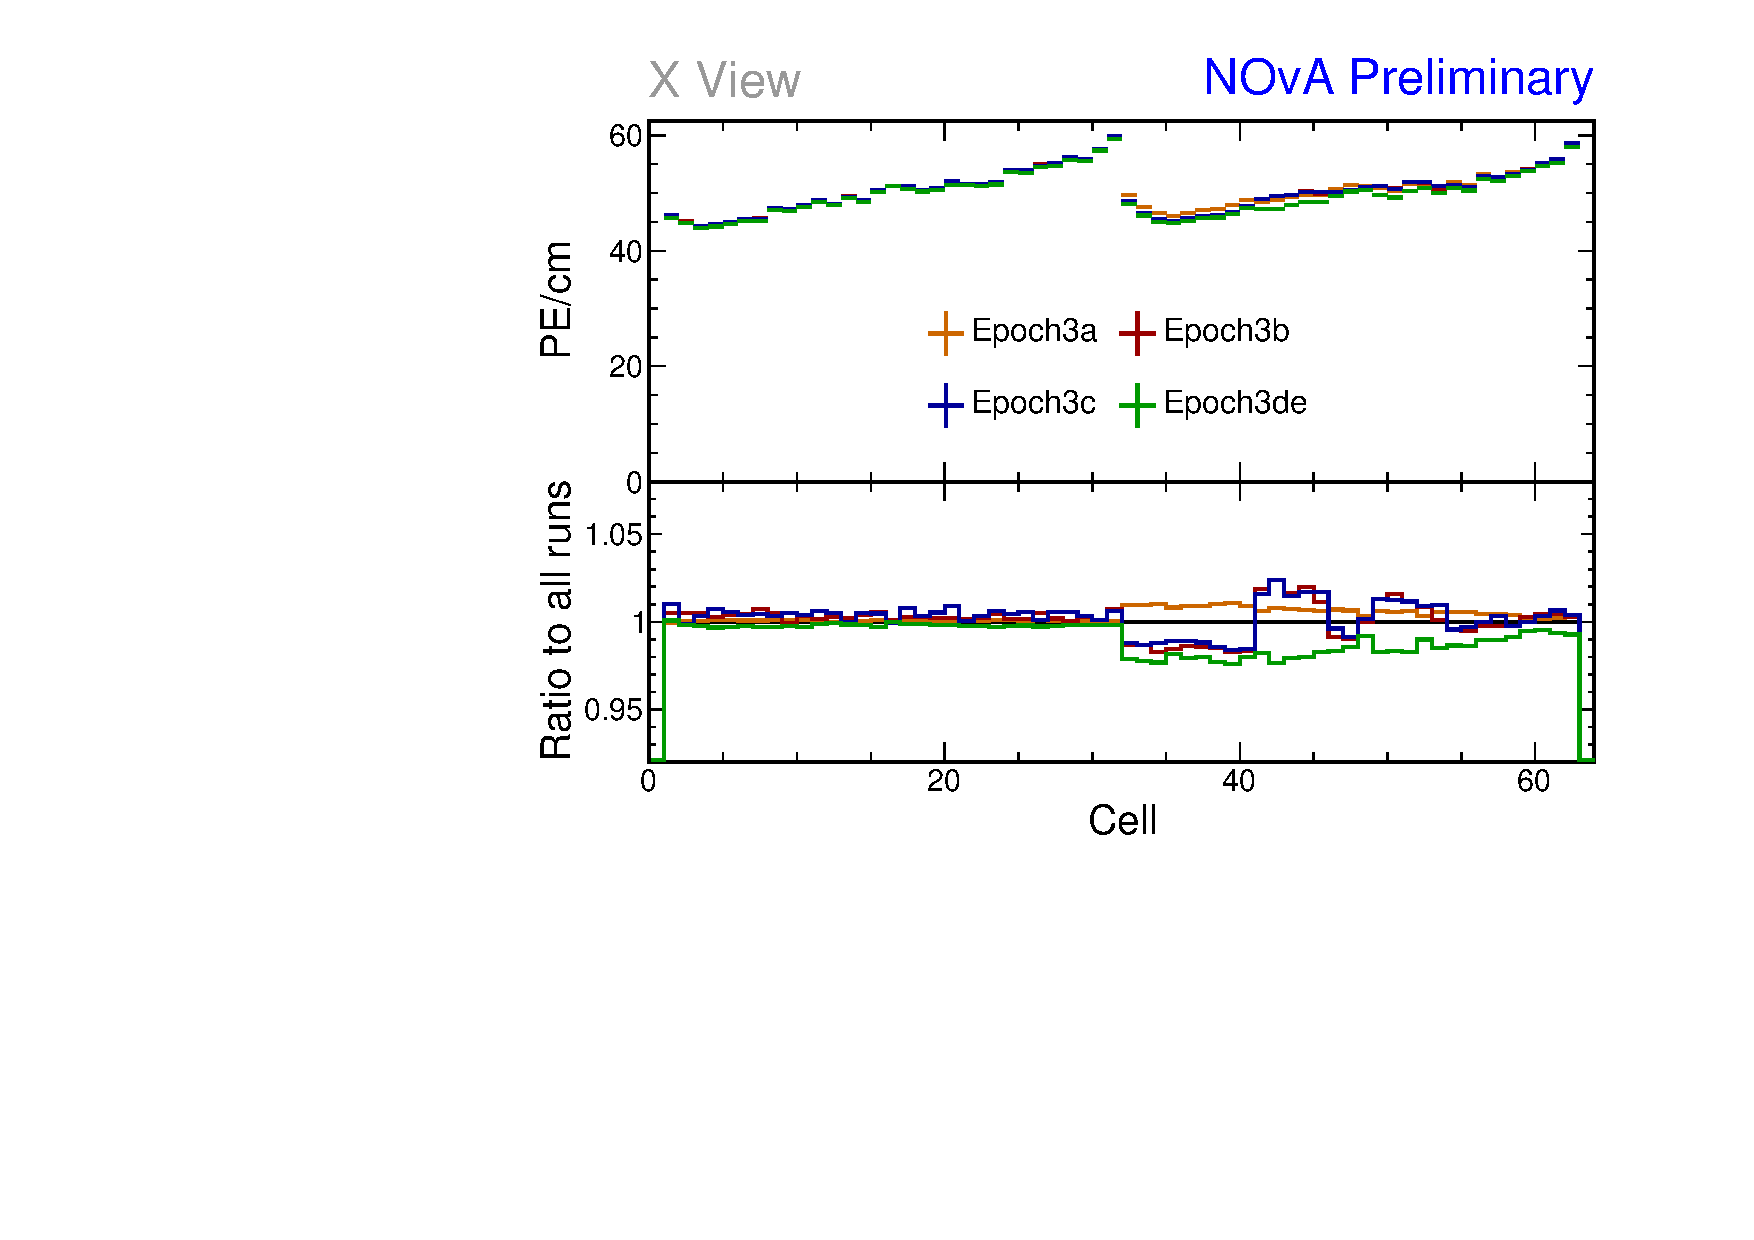
\includegraphics[width=\textwidth]{Plots/TBCalibration/Attenprofs_P3Data_CellPE_X_Combined.pdf}
\end{subfigure}
\begin{subfigure}[b]{0.495\textwidth}
\centering
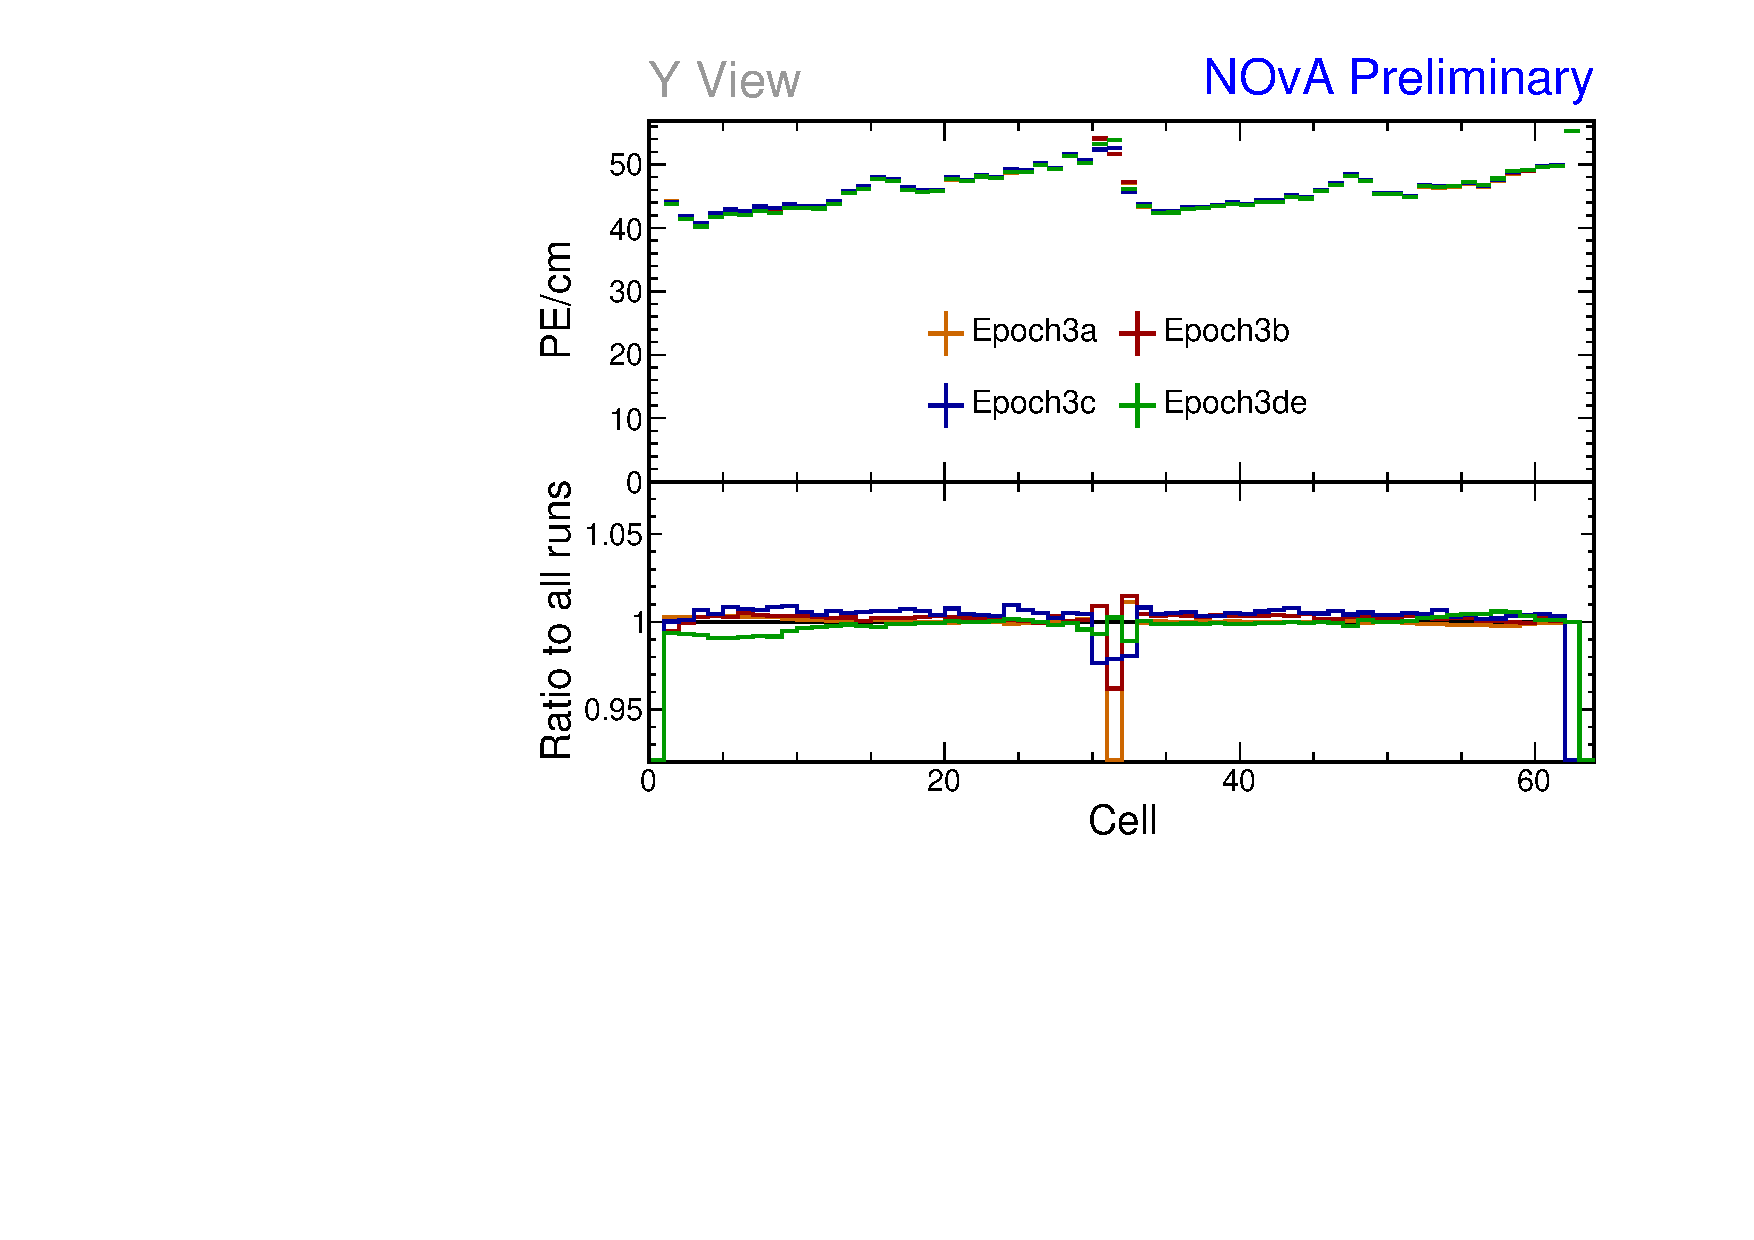
\includegraphics[width=\textwidth]{Plots/TBCalibration/Attenprofs_P3Data_CellPE_Y_Combined.pdf}
\end{subfigure}
\begin{subfigure}[b]{0.495\textwidth}
\centering
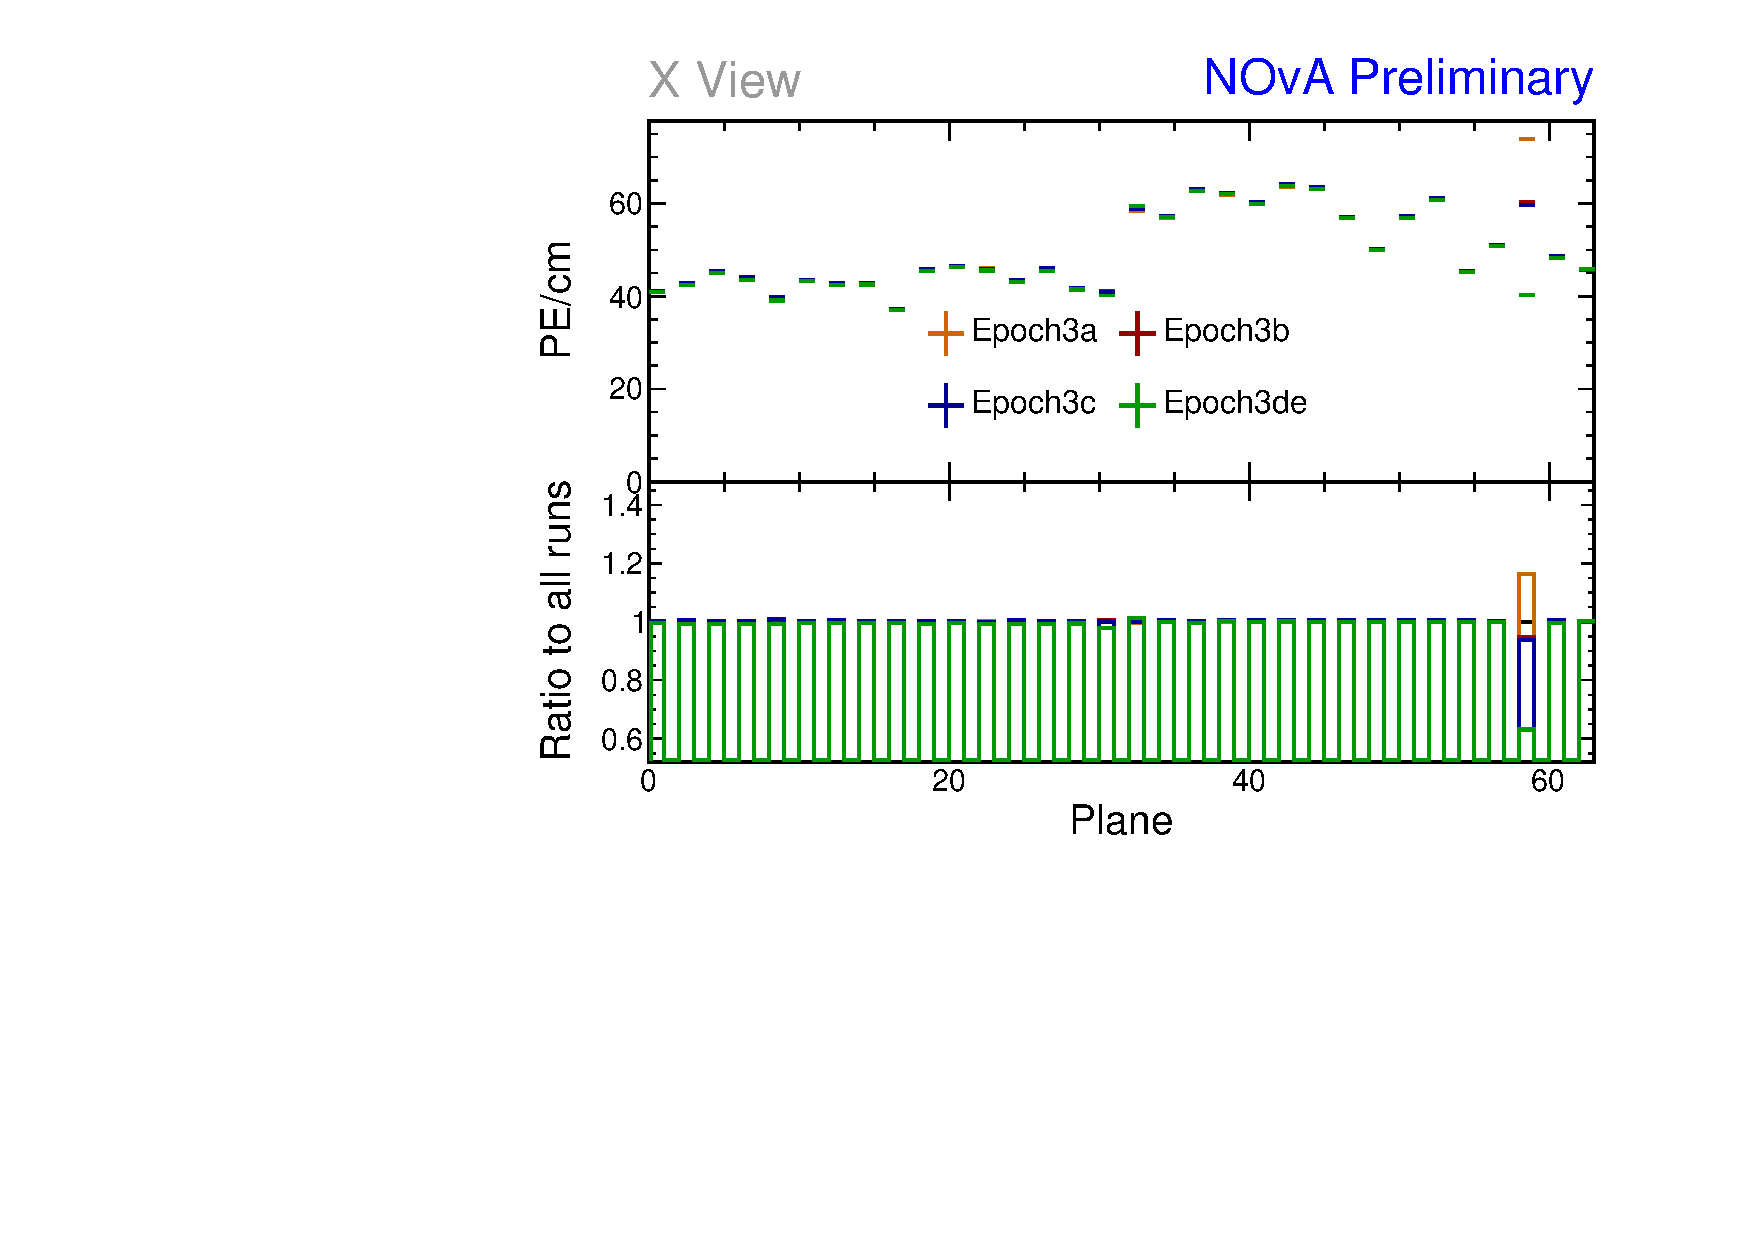
\includegraphics[width=\textwidth]{Plots/TBCalibration/Attenprofs_P3Data_PlanePE_X_Combined.pdf}
\end{subfigure}
\begin{subfigure}[b]{0.495\textwidth}
\centering
\includegraphics[width=\textwidth]{Plots/TBCalibration/Attenprofs_P3Data_PlanePE_Y_Combined.pdf}
\end{subfigure}
\caption[Uncorrected energy response along $w$, cell and plane for period 3]{Uncorrected average energy response as a function of the position within a cell ($w$ - top), cell number (middle), or plane number (bottom) for various epochs in the Test Beam detector period 3 data of cosmic muons hits selected for calibration. Left side shows distributions for the X view (vertical) planes and right side for the Y view (horizontal) planes. Each plot is a profile histogram, with uncertainties representing statistical variations. The effect of staged refilling of the underfilled cells between the epochs can be seen in the middle right plot, where epoch 3a (orange) has all no underfilled cells refilled, and epochs 3d and 3e (green) have all the cells filled to the top. Comparing the distributions of energy deposition in X view between the cell and plane plots, it can be seen that the top \acrshort{FEB}/\acrshort{APD} in plane 58, which correspond cells 32-63, was faulty throughout period 3. Specifically, that the energy response in this module was larger in epoch 3a, then got lower in epochs 3b and 3c, until getting significantly lower for epochs 3d and 3e.}
\label{fig:Calibhist_period3}
\end{figure}

From the aforementioned considerations, we decided to calibrate epochs 3a, 3b and 3c together, which are all the epochs containing any underfilled cells, and to separately calibrate epochs 3d and 3e together. The faulty \gls{FEB} in the top of plane 58 is far enough in the back of the detector, that we didn't find it necessary to calibrate epochs 3d and 3e separately. Additionally, epochs 3b and 3c contain only few days worth of data, therefore they wouldn't have enough events for successful independent attenuation fits.

\subsection*{Combined epochs 3a, 3b and 3c relative calibration results}

The results of attenuation fits for the combined epochs 3a, 3b and 3c are summarised in Fig.~\ref{fig:CellCentreResponseEp3abc}, showing the map of the fitted response at the centre of each cell. There are 182 uncalibrated cells out of 4032, constituting 4.51\% of the detector, as shown in Tab.~\ref{tab:TestBeamEp3abcRelCalibResults}.

\begin{figure}[!hbtp]
\centering
\includegraphics[width=\textwidth]{Plots/TBCalibration/CellResponseAtCentre_epoch3abc_Limited_NOvAPlotStyle.pdf}
\caption[Map of fitted response at cell centre for epochs 3a, 3b and 3c data]{Overview of the relative calibration results for the Test Beam detector period 3, combined epochs 3a, 3b and 3c data. Each cell represents the result of the attenuation fit to the energy response in the centre of that cell. The blank bins represent uncalibrated cells. The rows of uncalibrated cells 31 and 62 are caused by the underfilled cells together with the tricell condition. The same effect affects cell 32 in plane 1. The two dark-red stripes correspond to two faulty \glspl{FEB} in planes 36 and 58. There are five additional uncalibrated cells, specifically cell 2 in plane 58, cells 21 and 32 in plane 60, and cells 31 and 38 in plane 63, which are uncalibrated due to large fluctuations at cell edges.}
\label{fig:CellCentreResponseEp3abc}
\end{figure}

\begin{table}[!hbtp]
\centering
\caption[Summary of relative calibration results for the combined epochs 3a, 3b and 3c]{Summary of relative calibration results for the combined epochs 3a, 3b and 3c with the uncalibrated cells divided into four categories based on the main reason of failure, all described in text.}
\def\arraystretch{1.4}
\begin{tabular}{|cl|c|c|}
\hline
\multicolumn{2}{|c|}{\textbf{Calibration status}} & \textbf{Number of cells} & \textbf{Detector proportion}\\\hline
\multicolumn{2}{|c|}{Calibrated} & $3850$ & $\unit[95.49]{\%}$\\\hline
\parbox[t]{2mm}{\multirow{4}{*}{\rotatebox[origin=c]{90}{Uncalibrated }}} & Peripheral cells & $128$ & $\unit[3.17]{\%}$\\
 & Underfilled cells & $49$ & $\unit[1.22]{\%}$\\
 & Readout & $0$ & $\unit[0.00]{\%}$\\
 & Binning & $5$ & $\unit[0.12]{\%}$\\\hline
\end{tabular}
\label{tab:TestBeamEp3abcRelCalibResults}
\end{table}

We can see that some of the underfilled cells that have been refilled for epochs 3b or 3c, but were underfilled for epoch 3a, which makes up the majority of this calibrated data, are now calibrated thanks to including these two short epochs into the same attenuation fit. Example of energy deposition in such a cell is shown on the left side of Fig.~\ref{fig:AttenfitResultsEpoch3abc_UnderfilledCellsNeighbours}. Same as in period 2, most of the neighbouring cells to the underfilled cells are calibrated, except for cells on the edge of the detector due to lower statistics.

\begin{figure}[h]
  \begin{subfigure}{0.495\textwidth}
    \includegraphics[width=\linewidth]{Plots/RelativeCalibrationResults/ep3abc_005_031.png}
  \end{subfigure}
  \begin{subfigure}{0.495\textwidth}
    \includegraphics[width=\linewidth]{Plots/RelativeCalibrationResults/ep3abc_001_032.png}
  \end{subfigure}
  \caption[Attenuation fits for re-filled cells in period 3 data]{Fit to the energy response in epochs 3a, 3b and 3c. Some underfilled cells that have been refilled in epochs 3b and 3c are now calibrated as shown on the left plot. Cell 32 in plane 1 is the only neighbouring cell to the underfilled cell that didn't manage to get calibrated due to low number of events.}
  \label{fig:AttenfitResultsEpoch3abc_UnderfilledCellsNeighbours}
\end{figure}

There is a couple of noticeably faulty \glspl{FEB} with a scaled energy response, shown in Fig.~\ref{fig:AttenfitResultsEpoch3abc_FaultyFEBs}. Besides the expected \gls{FEB} in plane 58, which has about $5\times$ larger response, there is also the \gls{FEB} in plane 36, which has about $2.5\times$ larger response compared to the average. This could mean that the \gls{FEB} in plane 36 was faulty only for a limited time compared to the \gls{FEB} in plane 58. This is a reason for concern, as the relative calibration correction for hits in this module, during the time when the \gls{FEB} wasn't faulty, would be too large (and therefore the `corrected response' would be too small). On the other hand, during the time when the \gls{FEB} was faulty, the correction would be too small and hence the corrected response would be too large. Given that plane 36 is in the middle of the detector, there is a chance this might noticeably affect some Test Beam analysis results. Therefore, it is possible this issues might have to be mitigated in the future, whether with an additional uncertainty, or by improving the calibration. It is currently difficult to address issues such as this in the \gls{NOvA} calibration. However, there is currently an effort underway to split the inputs for calibration by cells, rather than by time, which would make solving these issues much simpler. For the time being, we decided to ignore these faulty \glspl{FEB}.

\begin{figure}[h]
  \begin{subfigure}{0.495\textwidth}
    \includegraphics[width=\linewidth]{Plots/RelativeCalibrationResults/ep3abc_036_054.png}
  \end{subfigure}
  \begin{subfigure}{0.495\textwidth}
    \includegraphics[width=\linewidth]{Plots/RelativeCalibrationResults/ep3abc_058_048.png}
  \end{subfigure}
  \caption[Attenuation fits for cells with faulty readout in period 3 data]{Fit to the energy response in epochs 3a, 3b and 3c. The most obvious faulty FEBs that have a significantly larger energy response than their neighbours.}
  \label{fig:AttenfitResultsEpoch3abc_FaultyFEBs}
\end{figure}

Similarly to period 2, there are a few cells in the back of the detector that have a sharp rise in energy response at their edge, which causes their attenuation fit to fail the calibration condition. This can be seen in Fig.~\ref{fig:AttenfitResultsEpoch3abc_CellEdges}, where the significantly different mean responses at the edge bins is pulling the attenuation fit to incorrect values. Given this is concentrated in cells in the end of the detector, we decided to ignore this effect and leave these cells uncalibrated.

\begin{figure}[h]
  \begin{subfigure}{0.495\textwidth}
    \includegraphics[width=\linewidth]{Plots/RelativeCalibrationResults/ep3abc_058_002.png}
  \end{subfigure}
  \begin{subfigure}{0.495\textwidth}
    \includegraphics[width=\linewidth]{Plots/RelativeCalibrationResults/ep3abc_060_032.png}
  \end{subfigure}
  \caption[Attenuation fits for cells with large fluctuations in period 3 data]{Fit to the energy response in epochs 3a, 3b and 3c. Some cells are not calibrated due to large fluctuations at one edge of the cells.}
  \label{fig:AttenfitResultsEpoch3abc_CellEdges}
\end{figure}

\subsection*{Combined epochs 3d and 3e relative calibration results}

The attenuation fits results for epochs 3d and 3e are shown in Fig.~\ref{fig:CellCentreResponseEp3de}. There are 182 uncalibrated cells out of 4032 total cells, making up 4.51\% of the detector. The uncalibrated cells are now however almost entirely concentrated at the edges of the detector. Summary of the relative calibration results is shown in Tab.~\ref{tab:TestBeamEp3deRelCalibResults}.

\begin{figure}[!hbtp]
\centering
\includegraphics[width=\textwidth]{Plots/TBCalibration/CellResponseAtCentre_epoch3de_original_Limited_NOvAPlotStyle.pdf}
\caption[Map of fitted response at cell centre for epochs 3d and 3e data]{Overview of the relative calibration results for the Test Beam detector period 3, combined epochs 3d and 3e data. Each cell represents the result of the attenuation fit to the energy response in the centre of that cell. The blank cells are uncalibrated. The uncalibrated cells 30-32 in plane 17 and cells 5-7 in plane 63 are caused by a dead channel coupled with the effect of the tricell condition. The 8 previously underfilled cells 31 in planes 33, 35, 37, 41, 47, 49, 51 and 59 are uncalibrated due to the difference in the scintillator used for refilling, as described in text. There are 11 cells that are uncalibrated due to low number of events combined with the attenuation profile binning.}
\label{fig:CellCentreResponseEp3de}
\end{figure}

\begin{table}[!hbtp]
\centering
\caption[Summary of relative calibration results for the combined epochs 3d and 3e]{Summary of relative calibration results for the combined epochs 3d and 3e with the uncalibrated cells divided into four categories based on the main reason of failure, all described in text. Brackets show the number of cells that were originally calibrated (or uncalibrated, depending on the row) before the manual alteration of their $\chi^2$ values, as described in text. Proportions are calculated from the final cell counts.}
\def\arraystretch{1.4}
\begin{tabular}{|cl|c|c|}
\hline
\multicolumn{2}{|c|}{\textbf{Calibration status}} & \textbf{Number of cells} & \textbf{Detector proportion}\\\hline
\multicolumn{2}{|c|}{Calibrated} & $3858\ (3850)$ & $\unit[95.68]{\%}$\\\hline
\parbox[t]{2mm}{\multirow{4}{*}{\rotatebox[origin=c]{90}{Uncalibrated }}} & Peripheral cells & $126$ & $\unit[3.13]{\%}$\\
 & Underfilled cells & $31\ (39)$ & $\unit[0.77]{\%}$\\
 & Readout & $6$ & $\unit[0.15]{\%}$\\
 & Binning & $11$ & $\unit[0.27]{\%}$\\\hline
\end{tabular}
\label{tab:TestBeamEp3deRelCalibResults}
\end{table}

The expected effect of one of the two dead channels is shown in Fig.~\ref{fig:AttenfitResultsEpoch3de_LeftoverUnderfilledCell} together with some of the cells in the back of the detector, which have a rise or drop in energy deposition at their edge. This is similar to the effects seen in period 2 and epochs 3a+3b+3c and since it's again concentrated in the end of the detector, we ignore these cells and leave them uncalibrated.

\begin{figure}[h]
  \begin{subfigure}{0.495\textwidth}
    \includegraphics[width=\linewidth]{Plots/RelativeCalibrationResults/ep3de_017_031.png}
  \end{subfigure}
  \begin{subfigure}{0.495\textwidth}
    \includegraphics[width=\linewidth]{Plots/RelativeCalibrationResults/ep3de_017_032.png}
  \end{subfigure}
  \begin{subfigure}{0.495\textwidth}
    \includegraphics[width=\linewidth]{Plots/RelativeCalibrationResults/ep3de_050_018.png}
  \end{subfigure}
  \begin{subfigure}{0.495\textwidth}
    \includegraphics[width=\linewidth]{Plots/RelativeCalibrationResults/ep3de_062_006.png}
  \end{subfigure}  
  \caption[Attenuation fits for dead channels in period 3 data]{Fit to the energy response in epochs 3d and 3e. Top plots show the dead channel (left) and its immediate neighbour (right) affected by the tricell condition. Bottom plots show examples of cells with large fluctuations on their edges likely caused by low number of events combined with binning of attenuation profiles.}
  \label{fig:AttenfitResultsEpoch3de_LeftoverUnderfilledCell}
\end{figure}

Epochs 3d and 3e should have all the previously underfilled cells now refilled, but as can be seen in Fig. \ref{fig:CellCentreResponseEp3de}, there are several of these previously underfilled cells that are still uncalibrated. The energy deposition in these cells is shown in Fig.~\ref{fig:AttenfitResultsEpoch3de_RefilledDiscrepancy}. Here we can see that these cells have a fairly large discrepancy between the left and right sides of the cell. This is caused by using different scintillator oils for the initial filling and for the refilling (or overfilling). Specifically, as was described in Sec.~\ref{sec:TBExperiment}, these cells have been initially filled with the Ash River oil, or with the Texas oils, depending on the cell, which have a higher energy response compared to the \gls{NDOS} oil that was used for their overfilling. These scintillator oils clearly did not mix properly, which caused a discrepancy in the energy deposition in different parts of the cells.
\begin{figure}[h]
  \begin{subfigure}{0.495\textwidth}
    \includegraphics[width=\linewidth]{Plots/RelativeCalibrationResults/ep3de_033_031.png}
  \end{subfigure}
  \begin{subfigure}{0.495\textwidth}
    \includegraphics[width=\linewidth]{Plots/RelativeCalibrationResults/ep3de_059_031.png}
  \end{subfigure}
  \caption[Attenuation fits for cells with mixed scintillators in period 3 data]{Fit to the energy response in epochs 3d and 3e. The scintillator oil used for refilling of the underfilled cells has lower energy response than the oil used for the initial filling. These oils didn't mix properly causing a different energy response in the left and right side of the cell.}
  \label{fig:AttenfitResultsEpoch3de_RefilledDiscrepancy}
\end{figure}
This is a physical effect that should be accounted for in calibration, and, as we can see, the attenuation fits are actually performing reasonably well. Additionally, these cells are in the middle of the detector and leaving them uncalibrated would almost certainly have an impact on Test Beam analyses. The large $\chi^2$ value of the attenuation fit is most likely caused only by the unusual shape of the distribution, which the fit is not designed for. Therefore, we decided to manually change the $\chi^2$ values for these cells inside the csv tables (which hold the results of the attenuation fits), so that their $\chi^2<0.2$ and these cells are officially considered calibrated when applying the calibration results, even if they originally weren't. The map of the `corrected' distribution of the attenuation fit results for epochs 3d and 3e is shown in Fig.~\ref{fig:CellCentreResponseEp3de_updated}.

\begin{figure}[!hbtp]
\centering
\includegraphics[width=\textwidth]{Plots/TBCalibration/CellResponseAtCentre_epoch3de_Limited_NOvAPlotStyle.pdf}
\caption[Corrected map of fitted response at cell centre for epochs 3d and 3e data]{Overview of the final relative calibration results for the combined epochs 3d and 3e data after manually labelling the originally uncalibrated refilled cells as calibrated. Each cell represents the result of the attenuation fit to the energy response in the centre of that cell. The blank cells are uncalibrated and described in text.}
\label{fig:CellCentreResponseEp3de_updated}
\end{figure}

\section{Period 4 data}\label{sec:TBPeriod4}

The data collected during period 4 of the Test Beam run represent our best dataset, with nearly ideal detector conditions. There were a few commissioning runs in the very beginning of period 4, which uncovered some dead channels or faulty \glspl{FEB} that were immediately fixed. These initial runs constitute epoch 4a, shown on the top of Fig.~\ref{fig:CalibhistMap_period4}. Additionally, a few runs included studies where parts of the detector were masked to address \gls{FEB} saturation issues \cite{NOvA-doc-53658}, clearly visible in the middle of Fig.~\ref{fig:CalibhistMap_period4}. The bottom part of Fig.~\ref{fig:CalibhistMap_period4} shows the remainder of period 4 data, which do not have any noticeable faults in their hit distribution across the detector.

\begin{figure}[!hbtp]
\centering
\begin{subfigure}[b]{\textwidth}
\centering
\includegraphics[width=\textwidth]{Plots/TBCalibration/Attenprofs_P4Data_CellPlane_Epoch4a.pdf}
\end{subfigure}
\begin{subfigure}[b]{\textwidth}
\centering
\includegraphics[width=\textwidth]{Plots/TBCalibration/Attenprofs_P4Data_CellPlane_CellMasking.pdf}
\end{subfigure}
\begin{subfigure}[b]{\textwidth}
\centering
\includegraphics[width=\textwidth]{Plots/TBCalibration/Attenprofs_P4Data_CellPlane_GoodRuns.pdf}
\end{subfigure}
\caption[Plane-Cell distribution of hits for the period 4 data sample]{Distribution of events in the Test Beam period 4 data calibration sample. The top plot shows the first three commissioning runs with readout issues, the middle plot shows the status of the detector during the cell masking studies and the bottom plot shows the rest of the runs. Only the runs from the bottom plot (marked GoodRuns) are used for calibration.}
\label{fig:CalibhistMap_period4}
\end{figure}

Figure~\ref{fig:Calibhist_period4} shows, that the epoch 4a and the cell masking study had noticeable impacts on the energy deposition across the detector. Both of these special periods only span a short time and therefore contain very limited number of hits. We decided to ignore these runs and only calibrate the rest of period 4 data, using their results for all runs in period 4.

\begin{figure}[!hbtp]
\centering
\begin{subfigure}[b]{0.495\textwidth}
\centering
\includegraphics[width=\textwidth]{Plots/TBCalibration/Attenprofs_P4Data_WPE_corr_xy_X_Combined.pdf}
\end{subfigure}
\begin{subfigure}[b]{0.495\textwidth}
\centering
\includegraphics[width=\textwidth]{Plots/TBCalibration/Attenprofs_P4Data_WPE_corr_xy_Y_Combined.pdf}
\end{subfigure}
\begin{subfigure}[b]{0.495\textwidth}
\centering
\includegraphics[width=\textwidth]{Plots/TBCalibration/Attenprofs_P4Data_CellPE_X_Combined.pdf}
\end{subfigure}
\begin{subfigure}[b]{0.495\textwidth}
\centering
\includegraphics[width=\textwidth]{Plots/TBCalibration/Attenprofs_P4Data_CellPE_Y_Combined.pdf}
\end{subfigure}
\begin{subfigure}[b]{0.495\textwidth}
\centering
\includegraphics[width=\textwidth]{Plots/TBCalibration/Attenprofs_P4Data_PlanePE_X_Combined.pdf}
\end{subfigure}
\begin{subfigure}[b]{0.495\textwidth}
\centering
\includegraphics[width=\textwidth]{Plots/TBCalibration/Attenprofs_P4Data_PlanePE_Y_Combined.pdf}
\end{subfigure}
\caption[Uncorrected energy response along $w$, cell and plane for period 4]{Uncorrected average energy response as a function of the position within a cell ($w$ - top), cell number (middle), or plane number (bottom) for the Test Beam detector period 4 data of cosmic muons hits selected for calibration. Left side shows distributions for the X view (vertical) planes and right side for the Y view (horizontal) planes. Each plot is a profile histogram, with uncertainties representing statistical variations. The commissioning runs in epoch 4a and the runs during the cell masking studies have a visibly different energy deposition across all the shown variables compared to the rest of the period 4 runs.}
\label{fig:Calibhist_period4}
\end{figure}

\subsection*{Period 4 relative calibration results}

Results of the attenuation fits for period 4 are summarised in Fig.~\ref{fig:CellCentreResponsePeriod4} and Tab.~\ref{tab:TestBeamPeriod4RelCalibResults}. We can see that almost the entire detector is now calibrated, with only few exceptions on the edges of the detector and a single cell with an unusually high response at the edge (right plot of Fig.~\ref{fig:AttenfitResultsPeriod4}). We treated the formerly underfilled cells the same way as in epochs 3d and 3e, manually changing the $\chi^2$ of their attenuation fits inside the csv files to $<0.2$, therefore making them officially calibrated. There are 108 uncalibrated cells out of 4032, totalling 2.68\% of the detector.

\begin{figure}[!hbtp]
\centering
\includegraphics[width=\textwidth]{Plots/TBCalibration/CellResponseAtCentre_period4_original_Limited_NOvAPlotStyle.pdf}
\includegraphics[width=\textwidth]{Plots/TBCalibration/CellResponseAtCentre_period4_Limited_NOvAPlotStyle.pdf}
\caption[Map of fitted response at cell centre for period 4 data]{Overview of the relative calibration results for the Test Beam detector period 4 data. Top plot shows the results of the attenuation fit and bottom plot shows the final result for period 4 after manually labelling the originally uncalibrated refilled cells as calibrated. Each cell represents the result of the attenuation fit to the energy response in the centre of that cell. The blank cells are uncalibrated. The uncalibrated cells are concentrated on the edge of the detector, with a single cell 47 in plane 54 with an unusually high response at the edge of the cell. The 7 previously uncalibrated cells in the middle of the detector were artificially marked as calibrated after careful considerations.}
\label{fig:CellCentreResponsePeriod4}
\end{figure}

\begin{table}[!hbtp]
\centering
\caption[Summary of relative calibration results for period 4]{Summary of relative calibration results for period 4 with the uncalibrated cells divided into four categories based on the main reason of failure, all described in text. Brackets show the number of cells that were originally (un)calibrated before the manual alteration of their $\chi^2$ values, as described in text. Proportions are calculated from the final cell counts.}
\def\arraystretch{1.4}
\begin{tabular}{|cl|c|c|}
\hline
\multicolumn{2}{|c|}{\textbf{Calibration status}} & \textbf{Number of cells} & \textbf{Detector proportion}\\\hline
\multicolumn{2}{|c|}{Calibrated} & $3924 (3917)$ & $\unit[97.32]{\%}$\\\hline
\parbox[t]{2mm}{\multirow{4}{*}{\rotatebox[origin=c]{90}{Uncalibrated }}} & Peripheral cells & $97$ & $\unit[2.41]{\%}$\\
 & Underfilled cells & $10 (17)$ & $\unit[0.25]{\%}$\\
 & Readout & $0$ & $\unit[0.00]{\%}$\\
 & Binning & $1$ & $\unit[0.02]{\%}$\\\hline
\end{tabular}
\label{tab:TestBeamPeriod4RelCalibResults}
\end{table}

\begin{figure}[h]
  \begin{subfigure}{0.495\textwidth}
    \includegraphics[width=\linewidth]{Plots/RelativeCalibrationResults/p4_035_031.png}
  \end{subfigure}
  \begin{subfigure}{0.495\textwidth}
    \includegraphics[width=\linewidth]{Plots/RelativeCalibrationResults/p4_054_047.png}
  \end{subfigure}
  \caption[Attenuation fits for cells with mixed oils in period 4 data]{Fit to the energy response in period 4. Previously underfilled cells refilled with a scintillator of a different quality causing an unusual distribution of energy deposition (left). Unusually high energy response at the edge of the cell 47 (right).}
  \label{fig:AttenfitResultsPeriod4}
\end{figure}

\FloatBarrier
%%%%%%%%%%%%%%%%%%%%%%%%%%%%%%%%%%%%%%%%%%%%%%%%%%%%%%%%%%%%%%%%%%%%%%%%%%%%%%%
%%%%%%%%%%%%%%%%%%%%%%%%%%%%%%%%%%%%%%%%%%%%%%%%%%%%%%%%%%%%%%%%%%%%%%%%%%%%%%%
%%%
%%%                        Absolute calibration results
%%%
%%%%%%%%%%%%%%%%%%%%%%%%%%%%%%%%%%%%%%%%%%%%%%%%%%%%%%%%%%%%%%%%%%%%%%%%%%%%%%%
\section{Absolute calibration results}\label{sec:TBAbsoluteCalib}
The results of the relative calibration (without the threshold and shielding correction) are applied to the stopping muon sample to calculate the absolute energy scale,  which translates the energy response from \gls{PECorr} to $\unit{GeV}$, as described in Sec.~\ref{sec:NOvACalibration}. We apply the absolute calibration cuts to select minimum ionising muons, which represent a very well understood source of energy deposition. The absolute calibration cuts are mostly the same as for the other \gls{NOvA} detectors, selecting hits $1-\unit[2]{m}$ from the end of their tracks and removing uncalibrated and wrongly reconstructed hits by requiring non-zero path lengths, \gls{PE}$>0$, \gls{PECorr}$>0$, as well as \gls{PECorr}$\unit{/cm}<100$. Additionally, we constrain $w$ to a smaller allowed range: $-80<w<\unit[80]{cm}$, reflecting the smaller Test Beam cell length, removing hits approximately $\unit[0.5]{m}$ from each side of the detector.

Distributions of reconstructed and true energy responses, for both views, and for each data and simulation sample, are shown in Fig.~\ref{fig:AbsCalibNHitsMEU}. The mean of each of these distributions constitute the \gls{MEU}$_{\mathrm{Reco}}$ or \gls{MEU}$_{\mathrm{True}}$ values for both views. We calculate the statistical uncertainty on the \gls{MEU} values as the standard deviation of the corresponding distributions divided by the square root of the number of entries. To combine the result from the two views, we take the average over the view-dependent \gls{MEU} values to obtain the final \gls{MEU} value for each sample. This is the first time in the calibration chain where the two views, which were treated completely independently so far, are combined together. The uncertainties are added in the sum of squares. The total number of entries, the \gls{MEU} values for each sample and view, as well as the combined \gls{MEU} values with corresponding statistical uncertainties are shown in Tab.~\ref{tab:calib_summary_table}. Given the large number of entries in the energy response distributions, the statistical uncertainties on the \gls{MEU} values are negligible (around $0.05\%$). These are however not the final uncertainties of the absolute energy scale used in \gls{NOvA}. Instead, we use comparison to other standard candles, as was explained in Sec.~\ref{sec:NOvASystematics}.

\begin{figure}[h!]
  \begin{subfigure}{\textwidth}
    \centering
    \includegraphics[height=0.2\linewidth]{Plots/Calibana/legend.pdf}
  \end{subfigure}
  \vspace*{2mm}

  \begin{subfigure}{0.495\textwidth}
    \includegraphics[width=\linewidth]{Plots/Calibana/nhits_meu_x.pdf}
  \end{subfigure}
  \begin{subfigure}{0.495\textwidth}
    \includegraphics[width=\linewidth]{Plots/Calibana/nhits_meu_y.pdf}
  \end{subfigure}
  \begin{subfigure}{0.495\textwidth}
    \includegraphics[width=\linewidth]{Plots/Calibana/nhits_mev_x.pdf}
  \end{subfigure}
  \begin{subfigure}{0.495\textwidth}
    \includegraphics[width=\linewidth]{Plots/Calibana/nhits_mev_y.pdf}
  \end{subfigure}
  \caption[Reconstructed and true energy responses of stopping muons]{Distributions of the reconstructed (top) and true (bottom) energy response of stopping muons in the X (left) and Y (right) view within a $1-\unit[2]{m}$ track window from the end of their tracks. The mean of the reconstructed and true distributions of the response are the reconstructed and true MEU values respectively for the corresponding views.}
  \label{fig:AbsCalibNHitsMEU}
\end{figure}

\begin{table}[h!]
\centering
\caption[Summary of absolute calibration results]{Summary of absolute calibration results. \acrshort{MEU}$_{\mathrm{Reco}}$ values (top table), including the statistical uncertainty $\sigma_{\textsf{MEU}_{\mathrm{Reco}}}$, are in units of \acrshort{PECorr}$\unit{/cm}$ and \acrshort{MEU}$_{\mathrm{True}}$ values (bottom table) are in units of $\unit{MeV/cm}$}
\begin{tabular}{|c|c|c|c|c|c|c|c|}
\hline
\multicolumn{2}{|c|}{\multirow{2}{*}{Sample}} & \multicolumn{2}{c|}{X view} & \multicolumn{2}{c|}{Y view} & \multicolumn{2}{c|}{Combined}\\\cline{3-8}
\multicolumn{2}{|c|}{} & NHits & MEU & NHits & MEU & \cellcolor[HTML]{F8A102}MEU$_{\mathrm{Reco}}$ & $\sigma_{\textsf{MEU}_{\mathrm{Reco}}}$\\ \hline
 \parbox[t]{2mm}{\multirow{4}{*}{\rotatebox[origin=c]{90}{Data}}}
 & Period 2 & 2.322e+05 & 38.70 & 1.413e+06 & 39.40 & \cellcolor[HTML]{F8A102}39.05 & 0.02\\ \cline{2-8} 
 & Epochs 3abc & 2.638e+05 & 38.49 & 1.621e+06 & 39.40 & \cellcolor[HTML]{F8A102}38.94 & 0.02\\ \cline{2-8}
 & Epochs 3de & 1.049e+05 & 38.63 & 6.725e+05 & 39.42 & \cellcolor[HTML]{F8A102}39.02 & 0.03\\ \cline{2-8}
 & Period 4 & 5.268e+05 & 38.63 & 3.316e+06 & 39.40 & \cellcolor[HTML]{F8A102}39.01 & 0.01\\ \hline
\multicolumn{2}{|c|}{Simulation} & 2.829e+05 & 40.17 & 1.842e+06 & 39.93 & \cellcolor[HTML]{F8A102}40.05 & 0.02\\ \hline
\end{tabular}

\vspace*{2mm}
\begin{tabular}{|c|c|}
\hline
\cellcolor[HTML]{F8A102}MEU$_{\mathrm{True}}$ = 1.7722 $\unit{MeV/cm}$ & $\sigma_{\textsf{MEU}_{\mathrm{True}}}$ = 0.0003 $\unit{MeV/cm}$\\ \hline
\end{tabular}
\label{tab:calib_summary_table}
\end{table}

As expected, the comparison of the absolute calibration results in Fig.~\ref{fig:AbsCalibNHitsMEU} and Tab.~\ref{tab:calib_summary_table} demonstrates that the \gls{MEU} values across the four data samples are consistent, particularly in the Y view, which has larger statistics. However, the \gls{MEU}$_{Reco}$ values are noticeably higher for simulation than for data, especially in the X view (vertical planes). This discrepancy is anticipated, as through-going muons in the new data-based simulation (Sec.~\ref{sec:DataBasedSimulation}) have incorrect (smaller) incident energies, leading to smaller mean deposited energies  used in the attenuation fits and consequently larger relative calibration corrections. These larger corrections are then applied to the correctly simulated stopping muons, resulting in higher \gls{PECorr} and therefore larger \gls{MEU}$_{\mathrm{Reco}}$. Additionally, the true deposited energy, and therefore the \gls{MEU}$_{\mathrm{True}}$, which is also used for data, should be accurate.

%This is caused due to the data-based simulation we are using does not have a correct energy estimation for through-going muons, which have generally underestimated energies \cite{NOVA-doc-60026}. This results in an over-estimated correction from the relative calibration. However, this is not an issue, since we only use stopping muons to calculate the absolute energy scale and stopping muons have correct energies in the new simulation.

There is a noticeable discrepancy of about $\unit[1]{\%}$ in the \gls{MEU}$_{\mathrm{Reco}}$ values between the two views. Given the minimal statistical uncertainties and the consistency of results across the samples, this is unlikely to be a random effect. Additionally, the discrepancy between the two views is in a different direction for the data samples and for simulation. The actual reason for this discrepancy is unknown; it could be due to a real difference in the stopping muon distribution between the two views that is not accounted for, or a systematic difference in the calibration treatment of the two views. This effect is observed in all \gls{NOvA} detectors \cite{NOvA-doc-60709}. Since this means that the final result is technically incorrect for both views, one possible mitigation is to apply the absolute calibration results to each view separately. However, this contradicts the logic that stopping muons can serve as a standard candle, providing a single final calibration value.

%%%%%%%%%%%%%%%%%%%%%%%%%%%%%%%%%%%%%%%%%%%%%%%%%%%%%%%%%%%%%%%%%%%%%%%%%%%%%%%
%%%%%%%%%%%%%%%%%%%%%%%%%%%%%%%%%%%%%%%%%%%%%%%%%%%%%%%%%%%%%%%%%%%%%%%%%%%%%%%
%%%
%%%                      Final results and conclusions
%%%
%%%%%%%%%%%%%%%%%%%%%%%%%%%%%%%%%%%%%%%%%%%%%%%%%%%%%%%%%%%%%%%%%%%%%%%%%%%%%%%
\section{Validation}\label{sec:TBCalibValidation}

The initial validation of the Test Beam detector calibration is performed using the same cosmic muons that were used in the calibration process. This step is essential to ensure that the calibration performs as intended and successfully unifies the energy deposition of cosmic muons across the detector (as a function of $w$, cell and plane) and throughout the Test Beam detector runtime. By analysing these validation results and investigating any residual differences, we assess the stability and quality of the calibration.

After the initial validation with cosmic muons, we apply the calibration results to beam events. For the \gls{ND} and the \gls{FD}, we use a selection of standard candles, as described in Sec.~\ref{sec:NOvASystematics}, to evaluate the performance of the cosmic-based calibration on beam events and to assess the calibration systematic uncertainties. However, Test Beam offers a unique opportunity to validate the detector calibration directly with measurements from its beamline and to reassess and potentially reduce the systematic uncertainties associated with detector calibration in \gls{NOvA}. This is going to be one of the main results of the Test Beam experiment, therefore, we are focusing solely on the cosmic-based validation process.

The following section highlights the most important features observed during the validation, with additional plots provided in Appendix~\ref{sec:AppTBCalibValid} for the reader's convenience.

\subsection{Validation with stopping muons}

First, we examine the calibration effects on the same stopping muon hits as were used for the absolute calibration (Sec.~\ref{sec:TBAbsoluteCalib}), including all the absolute calibration cuts. These stopping muons, which have a very reliable and stable energy deposition, are used to compare the calibration performance amongst the various data and simulation samples. However, since we require hits to be within $\unit[1-2]{m}$ from the end of the stopping muons' tracks, they are not evenly distributed across the detector, particularly absent in its bottom parts. This causes large statistical uncertainties and scattered distributions along $w$ in the X view (for hits with $w<0$), and across cells in the Y view (for cells $<32$).

Figures \ref{fig:AbsCalibW1}-\ref{fig:AbsCalibDrift1} present the distributions of uncorrected (in \gls{PE}$\unit{/cm}$) and corrected (in $\unit{MeV/cm}$) energy deposition as a function of $w$, cell number, plane number, and time. The uncorrected energy deposition distributions are displaying the same general attributes as were discussed for each sample in previous sections. As expected, the corrected energy deposition is generally uniform across all the studied variables. However, some residual variations can be noticed and are discussed below.

% General w distribution - all good
The distributions as a function of $w$ (Fig.~\ref{fig:AbsCalibW1}) illustrate the successful uniformity of energy deposition after applying calibration. Excluding the region affected by the lack of stopping muon hits, the corrected energy deposition for each sample is uniform within $\pm\unit[0.5]{\%}$. Additionally, all four data samples are consistent with each other, and the discrepancy between data and simulation is within $\pm\unit[1.5]{\%}$.

\begin{figure}[!ht]
  \begin{subfigure}{\textwidth}
  \centering
    \includegraphics[height=0.2\linewidth]{Plots/Calibana/legend.pdf}
  \end{subfigure}
  \vspace*{2mm}
  
  \begin{subfigure}{0.495\textwidth}
    \includegraphics[width=\linewidth]{Plots/Calibana/pecm_w_x.pdf}
  \end{subfigure}
  \begin{subfigure}{0.495\textwidth}
    \includegraphics[width=\linewidth]{Plots/Calibana/pecm_w_y.pdf}
  \end{subfigure}
  \begin{subfigure}{0.495\textwidth}
    \includegraphics[width=\linewidth]{Plots/Calibana/recomevcm_w_x.pdf}
  \end{subfigure}
  \begin{subfigure}{0.495\textwidth}
    \includegraphics[width=\linewidth]{Plots/Calibana/recomevcm_w_y.pdf}
  \end{subfigure}
  \caption[Validation plots for stopping muons along w]{Distributions of uncorrected (top) and corrected (bottom) energy deposition for stopping \acrshort{MIP} muons in the X view (left) and the Y view (right) as a function of the position within a cell. Bottom panel of each plot shows the ratio of the simulation sample (gray) and the four data samples, labelled at the top. Ep3a labels a combination of epochs 3a+3b+3c and Ep3d labels epochs 3d+3e. The left half ($w<0$) of the X view distributions has large statistical uncertainties due to the low number of stopping muons at the bottom of the detector. The discrepancy between the data and the simulation samples for the corrected energy depositions is explained in text.}
  \label{fig:AbsCalibW1}
\end{figure}

% The uncorrected response is clearly getting lower with time
The distributions of uncorrected energy deposition as a function of $w$ (top of Fig.~\ref{fig:AbsCalibW1}) demonstrate a relative decrease in energy response over time, with period 4 data exhibiting a significantly smaller uncorrected energy response than period 2 data. This decrease, however, is corrected by calibration as expected.

% Generally different scale for simulation in X and Y views
The data-simulation discrepancy for the corrected energy deposition along $w$ (bottom of Fig.~\ref{fig:AbsCalibW1}) varies in the opposite direction between the X and Y views. This discrepancy arises from averaging the two view-dependent \gls{MEU}$_{\mathrm{Reco}}$ values, which show opposite variation in simulation compared to data, as explained in Sec.~\ref{sec:TBAbsoluteCalib}. Ideally, there should be no data-simulation discrepancy after applying the full calibration results. Therefore, applying the view-dependent absolute calibration results separately to each view, which would likely resolve this issue, is worthwhile to consider.

% Cell distributions - is this caused by the APD gains and the threshold correction?
The distributions of energy deposition across cells in Fig. \ref{fig:AbsCalibPlane1} exhibit greater variability after calibration compared to the $w$ dependence. This variability, particularly noticeable in the X view, is caused by issues with the threshold and shielding correction discussed in Sec.~\ref{sec:TBThresholdCorrection}. The threshold and shielding correction is not applied to these distributions, just as it is not applied to the stopping muon sample for absolute calibration or to beam events, as it is not supposed to affect them. However, since the incorrect threshold and shielding correction is applied during relative calibration, it is incorporated into the calibration results and consequently into the reconstructed deposited energy. The variability introduced by these faulty corrections is within $\pm\unit[3.5]{\%}$.

%Why does it appear there is a larger variation in the X view? Is it purely statistics?

\begin{figure}[!ht]
  \begin{subfigure}{\textwidth}
  \centering
    \includegraphics[height=0.2\linewidth]{Plots/Calibana/legend.pdf}
  \end{subfigure}
  \vspace*{2mm}

  \begin{subfigure}{0.495\textwidth}
    \includegraphics[width=\linewidth]{Plots/Calibana/pecm_cell_x.pdf}
  \end{subfigure}
  \begin{subfigure}{0.495\textwidth}
    \includegraphics[width=\linewidth]{Plots/Calibana/pecm_cell_y.pdf}
  \end{subfigure}
  \begin{subfigure}{0.495\textwidth}
    \includegraphics[width=\linewidth]{Plots/Calibana/recomevcm_cell_x.pdf}
  \end{subfigure}
  \begin{subfigure}{0.495\textwidth}
    \includegraphics[width=\linewidth]{Plots/Calibana/recomevcm_cell_y.pdf}
  \end{subfigure}
  \caption[Validation plots for stopping muons across cells]{Distributions of uncorrected (top) and corrected (bottom) energy deposition for stopping \acrshort{MIP} muons in the X view (left) and the Y view (right) as a function of the cell number. Bottom panel of each plot shows the ratio of the simulation sample (gray) and the four data samples, labelled at the top. Ep3a labels a combination of epochs 3a+3b+3c and Ep3d labels epochs 3d+3e. The left part (cell $\lesssim 25$) of the Y view distributions has large statistical uncertainties due to the low number of stopping muons at the bottom of the detector. Features described in text.}
  \label{fig:AbsCalibCell1}
\end{figure}

% Cell distribution in Y view - what is up with that middle cells - underfilled?
The distribution of corrected energy across cells in the Y view (bottom right of Fig.~\ref{fig:AbsCalibCell1}) additionally shows two cells with a noticeably lower energy response (\mbox{$\sim\unit[2-4]{\%}$}) for period 2 and epochs 3a+3b+3c compared to the rest of the samples. Specifically, this is the cell 31, which was underfilled during period 2 and epoch 3a, and its neighbouring cell 32. The variation for the underfilled cell is expected. However, it is unclear why one of the neighbouring cells to the underfilled cells is miscalibrated.

% Uncorrected energy response for different sammples - seems like the old scintillator is ageing the most, the Ash river the least and the Texas oil is somewhere in the middle
The relative differences in the uncorrected energy response across planes (top of Fig.~\ref{fig:AbsCalibPlane1}) between the three different data taking periods demonstrate that the decrease in energy deposition over time varies between planes. This variation is especially noticeable in the X view plot, but is equally present in the Y view planes. This effect is attributed to the differences in the quality of the scintillator oil used to fill the detector, as explained in Sec.~\ref{sec:TBExperiment}. Additionally, it indicates scintillator ageing, which results in a decrease of the scintillation light produced per deposited energy over time. Specifically, the \texttt{ND+NDOS} scintillator oil (planes 0-31) appears to have aged the most between periods 2 and 4, followed by the Texas \texttt{NDOS} oil (planes 53-62), while the Ash River oil (planes 32-52) aged the least. However, more quantitative studies are necessary to assess the ageing of the \gls{NOvA} scintillator, as its details are currently not well understood.

\begin{figure}[!ht]
  \begin{subfigure}{\textwidth}
  \centering
    \includegraphics[height=0.2\linewidth]{Plots/Calibana/legend.pdf}
  \end{subfigure}
  \vspace*{2mm}

  \begin{subfigure}{0.495\textwidth}
    \includegraphics[width=\linewidth]{Plots/Calibana/pecm_plane_x.pdf}
  \end{subfigure}
  \begin{subfigure}{0.495\textwidth}
    \includegraphics[width=\linewidth]{Plots/Calibana/pecm_plane_y.pdf}
  \end{subfigure}
  \begin{subfigure}{0.495\textwidth}
    \includegraphics[width=\linewidth]{Plots/Calibana/recomevcm_plane_x.pdf}
  \end{subfigure}
  \begin{subfigure}{0.495\textwidth}
    \includegraphics[width=\linewidth]{Plots/Calibana/recomevcm_plane_y.pdf}
  \end{subfigure}
  \caption[Validation plots for stopping muons across planes]{Distributions of uncorrected (top) and corrected (bottom) energy deposition for stopping \acrshort{MIP} muons in the X view (left) and the Y view (right) as a function of the plane number. Bottom panel of each plot shows the ratio of the simulation sample (gray) and the four data samples, labelled at the top. Ep3a labels a combination of epochs 3a+3b+3c and Ep3d labels epochs 3d+3e. Features described in text.}
  \label{fig:AbsCalibPlane1}
\end{figure}

% Plane distribution in X view - large discrepancy in ep3abc
The distribution of the corrected energy response across planes in the X view (bottom left of Fig.~\ref{fig:AbsCalibPlane1}) reveals a significantly smaller response ($\sim\unit[16]{\%}$) for epochs 3a+3b+3c in plane 36. This indicates that the relative calibration over-corrected the energy response due to through-going muons having an unusually high energy response (as shown in Fig. \ref{fig:AttenfitResultsEpoch3abc_FaultyFEBs}), but not the selected stopping muons. The most likely explanation is that the affected \gls{FEB} was `faulty' only for a certain period. Consequently, the corrected energy response would be accurate for the period when the \gls{FEB} was faulty, but would be under-estimated for the period when the \gls{FEB} functioned normally.

%Also planes 16 and 48, same as planes 17 49
%FB map tell Sim to simulation the FEBv5 lower than the rest, but readout simulation shifts it higher. That's why it is incorrect in the threshold correction and in simulation
We can observe the effect of different \gls{FEB} versions in both the corrected and uncorrected energy response distributions across planes, shown in Fig.~\ref{fig:AbsCalibPlane1}. Specifically, the \gls{FEB}v5 was used in planes 16, 17, 48 and 49, which is evident by the relatively larger corrected energy deposition, especially in the simulation and in the X view. Although this effect should be corrected during calibration, it is not, due to the incorrect incorporation of the variations between the \gls{FEB} versions in the simulation and its impact on the threshold and shielding correction, as discussed in Sec.~\ref{sec:TBThresholdCorrection}.

% Shape of plane distribution in X view
% Why are planes 2 (for all data periods) and planes 54 and 56 for all periods but ep3abc so much lower? But this seems to be only present of the stopping muons as will be explained below...
There are additional variations in the corrected energy deposition across planes (bottom of Fig.~\ref{fig:AbsCalibPlane1}). In the X view, there is a significant ($\sim\unit[6]{\%}$) drop in corrected energy response in planes 4 and 58, along with a smaller drop in some surrounding planes. The cause of this variation is unknown. However, it appears to be due to a discrepancy between through-going and stopping muons, as it disappears when analysing through-going muons, as explain below. In the Y view, the corrected response increases with planes  within the first half of the detector. This effect is only observed in data and not in simulation. The origin of this slope is unclear, however it is also absent when examining variations for through-going muons.

%Dependence in time - maybe also mention the systematic uncertainty?
%Large variability; Only normalizing mean; Visibly smaller uncorrected response in period 4, however the trend is not clear and the fluctuations are larger than the possible effect of detector ageing; Others addressed this by calibrating smaller samples; TB has more variability due to the environment and less stable detector running conditions; This provides an opportunity to test these effect as they are not well understood within NOvA
The distributions of energy deposition over time (Fig.~\ref{fig:AbsCalibDrift1}) reveal a complex dependency and significant variations. As shown, the calibration process currently only normalizes the mean of each calibrated sample, leaving time-dependent variations within the samples uncorrected. The uncorrected energy response is noticeably higher for period 2 compared to period 4, likely due to detector ageing, as previously discussed. However, there is no clear downward-going trend; the variations are larger than any consistent time-dependent pattern, except fir the second half of period 4.

\begin{figure}[!ht]
  \begin{subfigure}{\textwidth}
    \centering
    \includegraphics[height=0.2\linewidth]{Plots/Calibana/legend.pdf}
  \end{subfigure}
  \vspace*{2mm}
  
  \begin{subfigure}{0.495\textwidth}
    \includegraphics[width=\linewidth]{Plots/Calibana/pecm_time_x.pdf}
  \end{subfigure}
  \begin{subfigure}{0.495\textwidth}
    \includegraphics[width=\linewidth]{Plots/Calibana/pecm_time_y.pdf}
  \end{subfigure}
  \begin{subfigure}{0.495\textwidth}
    \includegraphics[width=\linewidth]{Plots/Calibana/recomevcm_time_x.pdf}
  \end{subfigure}
  \begin{subfigure}{0.495\textwidth}
    \includegraphics[width=\linewidth]{Plots/Calibana/recomevcm_time_y.pdf}
  \end{subfigure}
  \caption[Validation plots for stopping muons along time]{Distributions of uncorrected (top) and corrected (bottom) energy deposition for stopping \acrshort{MIP} muons in the X view (left) and the Y view (right) as a function of the event UNIX time (which starts at the beginning of the \acrshort{NOvA} data taking. Comparing the four data samples, labelled at the top. Ep3a labels a combination of epochs 3a+3b+3c and Ep3d labels epochs 3d+3e. Features described in text.}
  \label{fig:AbsCalibDrift1}
\end{figure}

In the \gls{ND} and \gls{FD} calibration, these time-dependent variations are partially addressed by reducing the size of the calibration samples to month-long epochs. This approach reduces variations in the calibrated energy deposition but generally results in larger portions of the detector being uncalibrated. However, this did not have a significant effect on the rate of calibrated cells for the \gls{ND} and \gls{FD} \cite{NOvA-doc-60838} and in the future can be explored for Test Beam detector as well. The \gls{ND} and \gls{FD} typically exhibit smaller variations in energy response over time compared to the Test Beam detector due to the Test Beam detector's less stable running conditions, such as larger fluctuations in temperature and humidity in the Test Beam hall.

The effect of these environmental factors on detector performance, along with scintillator and potential readout electronics ageing, are not well understood within \gls{NOvA}. As these effects are more pronounced in the Test Beam detector, and given the range of scintillator oils and readout electronics used, separating the effects of the individual factors is challenging and is currently the focus of ongoing studies \cite{NOvA-doc-59591}.

%%% PCListAna
\subsection{Validation with through-going muons}
To validate the calibration performance without the limitations imposed by stopping muons, we examine the effects of calibration on through-going muons, which were also used for the relative calibration. Unlike for to the stopping muon sample, we apply the threshold and shielding corrections for the through-going muons to truly verify the validity of the relative calibration process. Since the simulated through-going muons have incorrect incident energies, this validation focuses solely on variations in shape rather than scale.

% Stable runs - say that I'm only taking the data from stable runs
Considering the variability of detector performance over time, we use through-going muons collected during `stable runs' in period 4, as depicted in Fig.~\ref{fig:ValidStableRuns}. This period was selected by visually inspecting the time dependence of corrected energy deposition and choosing runs that correspond to seemingly stable energy deposition.

\begin{figure}[!ht]
  \centering
  \includegraphics[width=0.8\linewidth]{Plots/PCListAna/Period4StableRuns.pdf}
  \caption[Selection of stable runs from the period 4 Test Beam data]{Selection of stable runs from the period 4 Test Beam data. Showing the reconstructed energy response as a function of the run number for through-going cosmic muons. Shaded red area shows rejected runs.}
  \label{fig:ValidStableRuns}
\end{figure}

% Edge effects - show one plot and say it's taken care of by the calibration shape uncertainty (which I haven't done)
Furthermore, Fig.~\ref{fig:ValidLimW} shows significant variation of energy deposition at cell edges. This issue is addressed by the calibration shape systematic uncertainty discussed in Sec.~\ref{sec:NOvASystematics}. Therefore, for this validation study we ignore the edge variations, using the same $w$ limit as for the stopping muon sample:  $-80<w<\unit[80]{cm}$.

\begin{figure}[!ht]
  \centering
  \includegraphics[width=0.6\linewidth]{Plots/PCListAna/AbsCalCuts_TBData_p4_StableRuns.pdf}
  \caption[Removing edge hits for validation with through-going muons]{Removing edge hits for validation with through-going muons. Showing only events from the stable runs of the period 4 Test Beam cosmic data.}
  \label{fig:ValidLimW}
\end{figure}

With the aforementioned constraints, we expect uniform distributions with limited variations. Residual variations should be scattered throughout the detector without any particular pattern, indicating potential errors in the calibration process. It is worth noting that investigating these distributions without applying the threshold and shielding correction led to the discovery of the issues discussed in Sec.~\ref{sec:TBThresholdCorrection}. Any remaining variations point to potential systematic uncertainties in the calibration process.

Figure~\ref{fig:ValidPCListAnaProfDists} displays individual distributions of corrected energy response as a function of $w$, plane, and cell number for both data and simulation. For through-going muons with the threshold and shielding correction applied, the calibration procedure works as expected, with residual variations around $\pm\unit[0.2]{\%}$ for the $w$ and cell dependence. However, for plane dependence, these residual variations are larger: approximately $\pm\unit[0.5]{\%}$ in data and up to $\pm\unit[1]{\%}$ in simulation. Additionally, maps of corrected energy deposition as a function of both plane and cell numbers, along with their 1D projections, are shown in Fig.~\ref{fig:ValidPCListAnaMapData} for data and in Fig.~\ref{fig:ValidPCListAnaMapSim} for simulation. These plots demonstrate that the final residual variations for calibration reach approximately $\unit[1]{\%}$ in data and $\unit[4]{\%}$ in simulation.

% Individual variations - very small
\begin{figure}[!ht]
  \begin{subfigure}{0.495\textwidth}
    \includegraphics[width=\linewidth]{Plots/PCListAna/DataAndSim_recomevcm_ts_w_X.pdf}
  \end{subfigure}
  \begin{subfigure}{0.495\textwidth}
    \includegraphics[width=\linewidth]{Plots/PCListAna/DataAndSim_recomevcm_ts_w_y.pdf}
  \end{subfigure}
  \begin{subfigure}{0.495\textwidth}
    \includegraphics[width=\linewidth]{Plots/PCListAna/DataAndSim_recomevcm_ts_cell_x.pdf}
  \end{subfigure}
  \begin{subfigure}{0.495\textwidth}
    \includegraphics[width=\linewidth]{Plots/PCListAna/DataAndSim_recomevcm_ts_cell_y.pdf}
  \end{subfigure}
    \begin{subfigure}{0.495\textwidth}
    \includegraphics[width=\linewidth]{Plots/PCListAna/DataAndSim_recomevcm_ts_plane_x.pdf}
  \end{subfigure}
  \begin{subfigure}{0.495\textwidth}
    \includegraphics[width=\linewidth]{Plots/PCListAna/DataAndSim_recomevcm_ts_plane_y.pdf}
  \end{subfigure}
  \caption[Validation plots for through-going muons as a function of w, cell and plane]{Distributions of through-going cosmic muons with $w\in\left(-80,80\right)\unit{cm}$ as a function of $w$, cells and planes for stable runs in the Test Beam period 4 data (black) and data-based simulation (red). Bottom panel of each plot shows the ratio between the value for each bin and the mean across the entire y axis, calculated separately for data and simulation.}
  \label{fig:ValidPCListAnaProfDists}
\end{figure}

\begin{figure}[!ht]
  \centering
  \includegraphics[width=0.7\linewidth]{Plots/PCListAna/TBDataP4_recomevcm_ts_zoomed.pdf}
  
  \includegraphics[width=0.7\linewidth]{Plots/PCListAna/Variation_recomevcm_TBDataP4_StableRuns_LimW.pdf}
  \caption[Map of corrected energy deposition for through-going cosmic muons in data]{Top: Map of corrected energy deposition for through-going cosmic muons with $w\in\left(-80,80\right)\unit{cm}$ as a function of cell and plane numbers for stable runs in the Test Beam period 4 data. Bottom: Projection of each bin from the map. Red line shows the median value of the projection and red shaded area shows the $\pm\unit[1]{\%}$ range of the median value. Gray shaded bins show the excluded bins corresponding to faulty \acrshort{FEB}, visible as a stark red line in plane 19 on the map. Additional features explained in text.}
  \label{fig:ValidPCListAnaMapData}
\end{figure}

\begin{figure}[!ht]
  \centering
  \includegraphics[width=0.7\linewidth]{Plots/PCListAna/TBSimulation_CP_recomevcm_ts_zoomed.pdf}
  
  \includegraphics[width=0.7\linewidth]{Plots/PCListAna/Variation_recomevcm_TBSimulation_LimW.pdf}
  \caption[Map of corrected energy deposition for through-going cosmic muons in simulation]{Top: Map of corrected energy deposition for through-going cosmic muons with $w\in\left(-80,80\right)\unit{cm}$ as a function of cell and plane numbers for stable runs in the Test Beam data-based simulation. Bottom: Projection of each bin from the map. Red line shows the median value of the projection and red shaded area shows the $\pm\unit[4]{\%}$ range of the median value. Additional features explained in text.}
  \label{fig:ValidPCListAnaMapSim}
\end{figure}

% Variations in data
In the distributions for data, we observe a clear effect of the different scintillators used, which is related to varying levels of detector ageing among the scintillators, as previously discussed. This effect is particularly noticeable in this validation sample due to the selection of events from `stable runs', while the relative calibration was calculated for the entire period 4. Therefore, calibration scales the deposited energy with respect to the mean deposited energy for the full period 4. Consequently, planes 0-31 appear to have the lowest relative corrected response in Fig.~\ref{fig:ValidPCListAnaProfDists} and \ref{fig:ValidPCListAnaMapData} because the corresponding \texttt{ND+NDOS} scintillator oil aged the most compared to the mean. This issue could be addressed by splitting period 4 into smaller epochs for calibration.

% Variations in simulation
For simulation, the relative calibration is performed in bins of $w$ for each cell and each \gls{FB} bin but importantly not for each plane. As a result, the relative calibration in simulation does not specifically correct for plane dependence, leading to larger variations between planes.

Furthermore, one half of plane 19 in data shows a corrected energy response approximately $\unit[0.7]{\%}$ higher than the rest. This is due to a faulty \gls{FEB} that was likely malfunctioning for a brief period. Since this study aims to examine purely the residual variations from the calibration procedure, cells corresponding to this \gls{FEB} can be ignored. Additionally, planes 48 and 49 in simulation, which correspond to \gls{FEB}v5, display a corrected energy response about $\unit[2-2.2]{\%}$ higher than the rest. This discrepancy arises from the incorrect accounting for different \gls{FEB} versions in simulation, combined with consolidating the planes into \gls{FB} bins.

\section{Summary}\label{sec:TBCalibSummary}

%Everything was great
I have successfully calibrated the NOvA Test Beam detector in four independent Test Beam data samples and in simulation. This is a critical step in order to analyse the Test Beam data, enabling crucial improvements to our understanding of the detector response and particularly of the calibration for all the \gls{NOvA} detectors.

Each calibrated sample contains only a few uncalibrated cells, mainly concentrated on the periphery of the detector. Most of the other uncalibrated cells failed the calibration condition due to unavoidable circumstances, such as underfilled cells, or dead channels. However, several improvements could increase the number of calibrated cells or otherwise improve the calibration performance. Some of the improvements could benefit not only the Test Beam detector but all the \gls{NOvA} detectors. These are especially the improved threshold and shielding correction, the individual treatment of cells during calibration, or the time variation studies of the \gls{NOvA} scintillator and electronics at the Test Beam detector, all outlined below.

%%% Threshold and shielding corrections and simulation issues - all NOvA
Several issues discovered during the Test Beam calibration that will enhance calibration and simulation for all the \gls{NOvA} detectors include the problems found with the threshold and shielding correction and with the readout simulation, described in Sec.~\ref{sec:TBThresholdCorrection}. Ongoing work aims to address these issues by improving the logic of the threshold and shielding correction or basing it entirely on data. Additionally, plans are in place to remove the relative gain variation from the simulation, as the \gls{FB} map used during simulation already sufficiently describes the relative gain variations, making the current treatment redundant.

%%% Faulty FEBs - transpose files - all NOvA, but might be complicated for FD
One of the most common issues that could be resolved is the faulty \glspl{FEB}, which often malfunctioned only for a limited period. This is particularly concerning, as cells belonging to faulty \glspl{FEB} usually pass the calibration condition; however, if the corresponding \gls{FEB} was faulty only for a limited period, the calibration results for those cells would be incorrect. This issue is currently difficult to address because the inputs for the relative calibration are organized by run and subrun numbers instead of by cells, making it impossible to calibrate cells corresponding to a single \gls{FEB} separately from the rest. However, ongoing work is adapting both the input files and the calibration procedures to enable calibrating individual cells separately.

%%% Time dependece - needs to be studied further, unique opportunity to understand this in all of nova, can be addressed by splitting
The time dependence of energy deposition in the Test Beam detector discussed in Sec.~\ref{sec:TBCalibValidation} is currently being studied and could help explain several contributions to the time-dependency seen in all \gls{NOvA} detectors. Specifically, the Test Beam can study the environmental effects on energy deposition, as well as the ageing of different scintillators and electronics. The first results indicate that the \gls{NOvA} scintillator oils age differently based on their quality. 

Addressing the time-dependent variations in the energy deposition in Test Beam could include splitting the calibrated periods into smaller samples, similarly to the \gls{ND} and \gls{FD}, which are using month-long samples for calibration. However, this approach risks insufficient statistics for attenuation fits in various cells. This could in turn be addressed by tuning the binning of the attenuation profiles to better fit the real cell dimensions that are actually being fitted in the attenuation fits.

%%% Better binning
%Several cells have failed the calibration condition due to a combination of low statistics and improper binning in the attenuation profiles. To  correct the dependence on time, the idea is to use smaller samples calibration, this effect could be enlarged. It's possible to partially tackle it by improving the binning of the attenuation profiles t
%Other suggestion for improvement is to change the binning of profile histograms to avoid the issues of single strange bins on the edges of the attenuation fit.

%%% Manually changing the chi2
Another technical improvements to the calibration results could stem from manually altering the $\chi^2$ value of cells that have attenuation fits which visibly looks all right, to below $0.2$. This would officially rendering these cells calibrated, similarly to how it was done for some cells in epochs 3d+3e and period 4. However, this would require manually going over all the uncalibrated cells, which is only really possible for the Test Beam detector and only for larger calibrated samples. Reducing the size of the calibrated sample would make this extremely impractical.

%Philosophical question of whether to manually change the chi2 values just cause by eye the response looks all right.

%%% Applying the absolute calibration for the views separately
Lastly, there is a possible improvement to the data-simulation discrepancy, by applying the absolute calibration results to each view independently. This would however have to be seriously considered, as the stopping muon sample used for calibration should technically not have any variation between the views and therefore this might introduce bias when applying the calibration results to beam data.
%Also applying the absolute calibration to the two views independently. - Is this actually what we'd want? Can still discuss it here...

%%% Possibly using Test Beam data to calculate the absolute energy scale

%%% Systematics
%Also have to devise proper systematic uncertainty for the TB calibration.
%We haven't attempted to estimate the uncertainty of the calibration, although we can estimate the final residual variations after applying the calibration. However, more work will need to go into this,  specifically to understand the time dependence of the deposited energy and the edge effects.

Overall, the calibration of the \gls{NOvA} Test Beam detector was successful and represents a significant advancement, with ongoing efforts aimed at further refining the process and addressing the identified issues to improve calibration accuracy and reliability across all \gls{NOvA} detectors. Part of the ongoing work also aims to quantify the correctness of the Test Beam calibration, devising a concrete systematic uncertainty.

As a result of this effort, \gls{NOvA} will be able to improve its analyses by reducing calibration-related systematic uncertainties. One key improvement is the ability to assess the absolute energy scale uncertainty - the largest of the calibration-related systematic uncertainties - separately for different particle types. Existing studies indicate that this uncertainty could be reduced from an overall $5\%$ to approximately $1.5\%$ for muons and $3\%$ for electromagnetic showers \cite{NOVA-doc-53225}. However, these estimates require validation from the Test Beam experiment, which is expected to further refine and lower these uncertainties. Additionally, correcting for threshold and shielding effects, along with other proposed calibration improvements, will likely enhance the calibration performance and reduce variations between detector cells.

%%% Discussion - Systematic uncertainties

%Variation of the MIP muons energy deposition between 1-2 m from their track end is about 1.8\% \cite{AbsCal_technote_1stAna.pdf}.

%\cite{AbsCal_technote_1stAna.pdf} Sources of systematic uncertainty of particular concern are those introduced by residual variations remaining after calibration. Systematic errors are introduced by spatial and temporal variations in detector response. Further, any difference between the two detectors may introduce a relative shift in the energy scale between the detectors. Track end misreconstruction: For a track window starting at 100 cm from the track end, a conservative mis-reconstruction of the track end point by 10cm will shift the start of the track window to between 90cm and 110cm. This shift will alter the MEU value by less than 0.4\% over the range. Variations in space and time: If the calibration procedure was ideal the detector response would not vary with position in either data or MC. The calibration is not ideal and the detector response and recorded simulated energy deposition varies with position of the hit within the detector, such variations will introduce systematic errors. The position of a hit can be defined by the plane, cell within the plane, and distance along the